\graphicspath{{./chapters/chapter2/}}

\chapter{Communication-Efficient Triangle Counting under Local Differential Privacy}\label{chap:2}

%\newcommand{\nats}{\mathbb{N}}
%\newcommand{\nnints}{\mathbb{Z}_{\ge0}}
%\newcommand{\reals}{\mathbb{R}}
%\newcommand{\nnreals}{\mathbb{R}_{\ge0}}
%\newcommand{\argmax}{\operatornamewithlimits{argmax}}
%\newcommand{\argmin}{\operatornamewithlimits{argmin}}

\def\bd{\bar{d}}
\def\bbma{\bar{\bma}}
\def\hd{\hat{d}}
\def\hf{\hat{f}}
\def\hg{\hat{g}}
\def\hr{\hat{r}}
\def\hw{\hat{w}}
\def\td{\tilde{d}}
% \def\AlgOne{\textsf{PrivSampleFullDwnld}$_{\triangle}$}
% \def\AlgTwo{\textsf{PrivSampleHalfNoisyDwnld}$_{\triangle}$}
% \def\AlgThree{\textsf{PrivSampleBothNoisyDwnld}$_{\triangle}$}
% \def\AlgOne{\textsf{ARRFullDL}$_{\triangle}$}
% \def\AlgTwo{\textsf{ARROneNoisyDL}$_{\triangle}$}
% \def\AlgThree{\textsf{ARRTwoNoisyDL}$_{\triangle}$}
% \def\AlgSec{\textsf{RRFullDL}$_{\triangle}(d_{max})$}
\def\AlgOne{\textsf{ARRFull}$_{\triangle}$}
\def\AlgTwo{\textsf{ARROneNS}$_{\triangle}$}
\def\AlgThree{\textsf{ARRTwoNS}$_{\triangle}$}
\def\AlgSec{\textsf{RRFull}$_{\triangle}(d_{max})$}
\newcommand{\GPlus}{\textsf{Gplus}}
\newcommand{\CostDL}{\mathrm{Cost}_{DL}}
\newcommand{\CostUL}{\mathrm{Cost}_{UL}}


\section{Introduction}
\label{chap2-sec:intro}
Counting subgraphs (e.g., triangles, stars, cycles) is
% a fundamental task 
one of the most basic tasks 
for analyzing connection patterns
% for analyzing graph statistics
in
% a graph.
various graph data, e.g., social,
communication, and collaboration networks.
% , epidemiological networks.
% Graph statistics is important to understand the connection patterns in various graph data; e.g., social networks, collaboration networks,
% For example, a degree distribution in a social graph represents a distribution of the number of friends in the graph.
% A subgraph count (e.g.,
For example,
% a triangle count is the number of three nodes with three edges.
% A $k$-star count is the number of a node connected to $k$ other nodes.
a triangle is given by a set of three nodes with three edges, whereas a $k$-star is given by a central node connected to $k$ other nodes.
% a set of $k$ nodes connected a central node.
These subgraphs
% are important because they can be used to calculate
play a crucial role in calculating
a \textit{clustering coefficient} ($=\frac{3 \times \text{\#triangles}}{\text{\#2-stars}}$) (see Figure~\ref{chap2-fig:triangles_stars}). 
% which 
The clustering coefficient 
measures the average probability that
two friends of a user will also be a friend
% a friend's friend is also a friend
in a social graph \cite{Newman_PRL09}. 
Therefore, it is useful for measuring the effectiveness of friend suggestions. 
In addition, the clustering coefficient represents the degree to which users tend to cluster together. 
Thus, if it is large in some services/communities, we can effectively apply social recommendations \cite{Kolluri_CCS21} to the users. 
% for an example of
% the triangle and $k$-star counts and clustering coefficient).
% these subgraph counts).
% \cite{Newman_PRL09}.
% It is also known that these subgraphs are sufficient statistics for exponential random graph models
Triangles 
and $k$-stars 
% can also be used for
are also useful for 
% modeling graphs \cite{Jorgensen_SIGMOD16,Robins_SN07}.
% generating graphs based on some
constructing
graph models
\cite{Robins_SN07,Jorgensen_SIGMOD16}; 
% and other applications \cite{Imola_USENIX21}.
% (e.g., exponential random graph models \cite{Robins_SN07}, TriCycle \cite{Jorgensen_SIGMOD16}).
% Applications of triangle counting are summarized in \cite{Tsourakakis_JGAA11}. 
see also \cite{Tsourakakis_JGAA11} for other applications of triangle counting. 
However, graph data often involve sensitive data such as sensitive edges (friendships),
% that a user wants to keep secret,
% which 
and they 
can be leaked from 
% exact values of triangle counts and $k$-star counts \cite{Imola_USENIX21}.
exact numbers of triangles and $k$-stars \cite{Imola_USENIX21}.
% Therefore,
% there is a need for
% we need to develop an algorithm for
% counting
% subgraphs while strongly protecting user privacy.
% , which is the focus of this paper.


To analyze subgraphs while protecting user privacy, DP (Differential Privacy) \cite{DP} has been widely adopted as a privacy metric \cite{Ding_TKDE21,Imola_USENIX21,Karwa_PVLDB11,Sun_CCS19,Ye_ICDE20,Ye_TKDE21,Zhang_SIGMOD15}.
DP protects user privacy against adversaries with arbitrary background knowledge and is known as a gold standard for data privacy.
% Most studies on private graph analysis \cite{Chen_PoPETs20,Day_SIGMOD16,Hay_ICDM09,Karwa_PVLDB11,Kasiviswanathan_TCC13,Nissim_STOC07,Raskhodnikova_arXiv15,Song_arXiv18} assumes central DP
According to the underlying model, DP can be categorized into \textit{central (or global) DP} and \textit{LDP (Local DP)}.
Central DP assumes a scenario where
% that
a central server has personal data of all users.
% whereas LDP does not assume such trusted servers.
Although accurate analysis of subgraphs is possible under
% central DP
this model \cite{Ding_TKDE21,Karwa_PVLDB11,Zhang_SIGMOD15}, there is a risk that the entire graph is leaked from the server by illegal access or internal fraud \cite{data_breach2021,CambridgeAnalytica}.
In addition, central DP cannot be applied to  \textit{decentralized social networks} 
\cite{Diaspora,Mastodon,Minds,Paul_CN14} 
% \cite{Diaspora,Mastodon,Paul_CN14} 
% (e.g., Diaspora \cite{Diaspora}, Mastodon \cite{Mastodon}) 
% which has no central server that has the entire graph, and uses many servers each of which has personal data of users who have registered
where the entire graph is distributed across many servers. 
% nor 
We can even consider 
\textit{fully decentralized applications} where a server does not have
any original edge, 
% between users, 
% information about the original edges;
% For example,
% mobile application in which each user sends the number of her friends
e.g., a mobile app that sends a noisy degree (noisy number of friends) to the server, which then estimates a degree distribution. 
Central DP cannot be used in such applications. 

In contrast, LDP assumes a scenario where each user obfuscates her personal data (friends list in 
the case of graphs) 
% data) 
by herself and sends the obfuscated data to a possibly malicious server; i.e., it does not assume trusted servers.
Thus, it does not suffer from a data breach and can also be applied to the decentralized applications. 
% explained above.
% LDP does not assume trusted servers, hence
% can be applied to the above decentralized applications.
% In LDP, each user obfuscates her personal data (friends list in the case of graph data) by herself, and sends the obfuscated data to a (possibly malicious) server.
% Since the server does not have the original data, it does not suffer from the data breach.
LDP has been widely studied in tabular data where each row corresponds to a user's personal data (e.g., age, browser setting, location) 
\cite{Acharya_AISTATS19,Bassily_NIPS17,Erlingsson_CCS14,Kairouz_ICML16,Murakami_USENIX19,Wang_USENIX17} 
% \cite{Acharya_AISTATS19,Bassily_NIPS17,Erlingsson_CCS14,Fanti_PoPETs16,Kairouz_ICML16,Murakami_USENIX19,Qin_CCS16,Wang_USENIX17}, 
and also in graph data \cite{Imola_USENIX21,Qin_CCS17,Ye_ICDE20,Ye_TKDE21}.
For example, $k$-star counts can be very accurately estimated under LDP because each user can count $k$-stars of which she is a center and sends a noisy version of her $k$-star count to the server \cite{Imola_USENIX21}.

However, more complex subgraphs such as triangles are much harder to count under LDP because each user
% is not aware of
cannot see
edges between other users.
For example, in Figure~\ref{chap2-fig:triangles_stars}, user $v_1$ cannot see
% an edge between $v_2$ and $v_3$,
edges between $v_2$, $v_3$, and $v_6$ 
and therefore 
% , hence 
cannot count triangles involving $v_1$.
Thus,
% when only one-round interaction is allowed between each user and the server,
% instead of sending a noisy triangle count,
existing algorithms \cite{Imola_USENIX21,Ye_ICDE20,Ye_TKDE21}
% send noisy edges (rather than noisy triangle counts) obtained by randomized response \cite{Warner_JASA65} to a server.
obfuscate each user's edges (rather than her triangle count) by
% Warner's
RR (Randomized Response)
% randomized response
\cite{Warner_JASA65} and send noisy edges to a server.
% , which then estimates the triangle count.
% \cite{Imola_USENIX21,Ye_ICDE20,Ye_TKDE21} apply Warner's RR (Randomized Response) \cite{Warner_JASA65}, which flips 0/1 with some probability, to each edge and then estimate the triangle count.
Consequently, the server suffers from a
% very
prohibitively
large estimation error
% as shown in \cite{Imola_USENIX21} and Appendix~\ref{chap2-sec:one-round} in our paper 
(e.g., relative error $> 10^2$ in large graphs, 
as shown in Appendix~\ref{chap2-sec:one-round}) 
% (e.g., relative error $> 10^2$ in large graphs, as shown in Appendix~\ref{chap2-sec:one-round} of our paper)
because all three edges are noisy in any noisy triangle the server sees.

\begin{figure}[t]
  \centering
  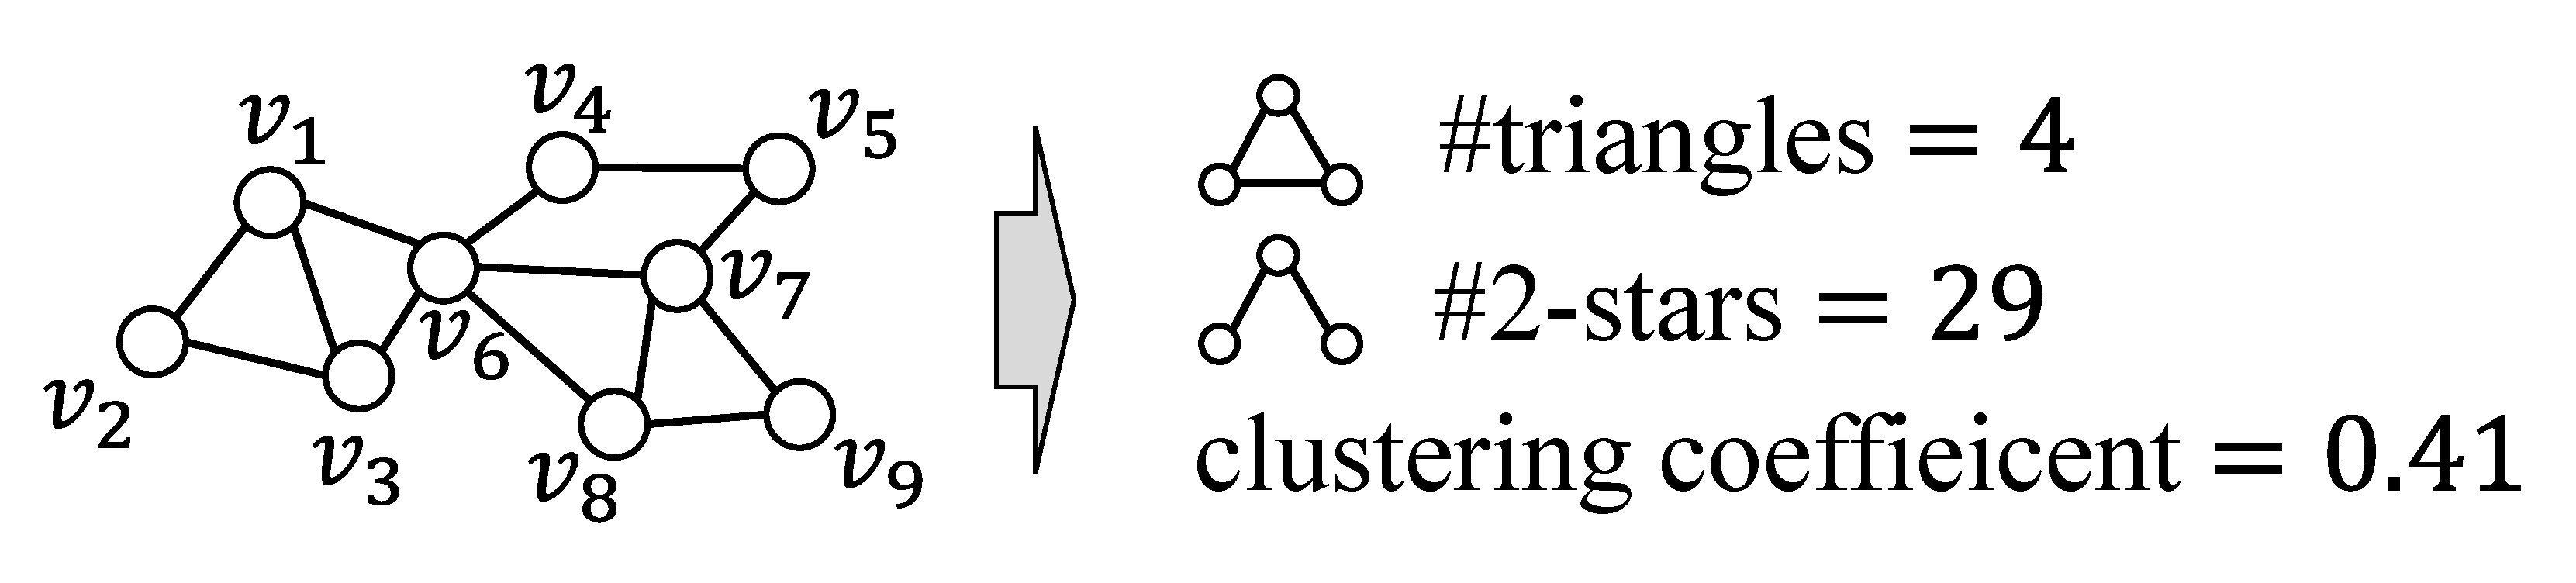
\includegraphics[width=0.85\linewidth]{fig/triangles_stars.pdf}
  
  \caption{Triangles, $2$-stars, and clustering coefficient.}
  \label{chap2-fig:triangles_stars}
\end{figure}

A recent study \cite{Imola_USENIX21} shows that the estimation error in
% triangle counting under LDP
locally private triangle counting
is significantly reduced by introducing an additional round of interaction between users and the server.
Specifically, if the server publishes the noisy graph (all noisy edges) sent by users at the first round, then each user can count her noisy triangles such that \textit{only one edge} is noisy (as she knows two edges connected to her).
Thus,
% each user
the algorithm in \cite{Imola_USENIX21} sends each user's noisy triangle count (with additional noise) to the server at the second round.
Then the server can accurately estimate the triangle count. 
% between users and the server 
% The algorithm in \cite{Imola_USENIX21} 
This algorithm also requires a much smaller number of interactions 
% between users and the server 
(i.e., only two) than collaborative approaches \cite{Kairouz_FTML21,Shokri_CCS15} that generally require many interactions. 

Unfortunately, 
% this algorithm 
the algorithm in \cite{Imola_USENIX21} 
is still
% far from practical
impractical 
for a large-scale graph.
% as shown in this paper.
Specifically, the noisy graph sent by users is dense, hence extremely large for a large-scale graph, e.g.,
$500$
% $400$
Gbits for a graph of
% about $900000$ users, as in our experiments).
a million users.
The problem is that \textit{every user} needs to download such huge data; e.g., when the download speed is $20$ Mbps (which is a recommended speed in YouTube \cite{YouTube_speed}), every user needs about 7 hours to download the noisy graph.
Since the communication ability might be limited for some users, the algorithm in \cite{Imola_USENIX21} cannot be
% applied to
used for
% a large-scale graph with diverse communication environments.
applications with large and diverse users.

In summary, existing triangle algorithms under LDP suffer from either a prohibitively large estimation error or a prohibitively 
% large 
high 
communication cost.
% For the same reason, they cannot calculate the clustering coefficient
They also suffer from the same issues when calculating the clustering coefficient.

% \colorB{
% \begin{itemize}
%     \item graph statistics; e.g., degree distribution, subgraph count (e.g., 2-stars, triangles), clustering coefficient.
%     \item privacy issue, DP, central DP, LDP.
%     \item 2-star counting under LDP is easy because...
%     \item triangle counting (hence clustering coefficient) is much harder because...
%     \item Previous work \cite{Imola_USENIX21}. Communication cost is prohibitively large (e.g., 400 Gbits for \IMDB{}).
%     \item This work
% \end{itemize}}

\smallskip
\noindent{\textbf{Our Contributions.}}~~We 
% In this work, we 
propose locally private triangle counting algorithms with a small estimation error and small communication cost.
% dramatically reduce the communication cost in accurate two-rounds triangle counting under LDP
% introduce some novel algorithms
% dramatically reduce the communication cost in locally private triangle counting
% address this issue
% by introducing some novel algorithms.
% Specifically, our contributions are:
Our contributions are as follows:

\begin{itemize}
    \item We propose two-rounds triangle algorithms
% that sample edges and then select edges each user downloads.
consisting of \textit{edge sampling} after RR and \textit{selecting edges each user downloads}.
In particular, we show that a simple extension of \cite{Imola_USENIX21} with edge sampling suffers from a large estimation error for a large or dense graph where the number of 4-cycles (such as $v_1$-$v_2$-$v_3$-$v_6$-$v_1$
% and $v_4$-$v_5$-$v_7$-$v_6$-$v_4$
in Figure~\ref{chap2-fig:triangles_stars}) is large.
To address this issue, we propose some strategies for selecting edges to download to reduce the error caused by the 4-cycles, which we call the \textit{4-cycle trick}.
\item We
show that
% the above algorithms
the algorithms with the $4$-cycle trick
still suffer from a large estimation error due to
% a large global sensitivity
% a large amount of the Laplacian noise.
large Laplacian noise for each user.
% To address this, 
To significantly reduce the Laplacian noise, 
we
propose a \textit{double clipping} technique,
which clips 
a degree (the number of edges) of each user 
% the number of edges 
with LDP and then clips the number of noisy triangles. 
% to significantly reduce the Laplacian noise.
% which significantly reduces the Laplacian noise by edge clipping and noisy triangle clipping.
% consists of edge clipping and noisy triangle clipping, to significantly reduce the global sensitivity in DP \cite{DP}.
% consisting of edge clipping and noisy triangle clipping
\item We evaluate our algorithms using two real datasets.
We show that our entire algorithms with the 4-cycle trick and double clipping
% provide the best performance, and
dramatically reduce the communication cost
% when compared with
of
\cite{Imola_USENIX21}.
For example,
% when the number of users is about $900000$,
for a graph with about $900000$ users,
we reduce the download cost from $400$ Gbits ($6$ hours when $20$ Mbps) to 
% $100$ Mbits ($5$ seconds) 
$160$ Mbits ($8$ seconds) or less 
while keeping the relative error much smaller than 1.
\end{itemize}
Thus, locally private triangle counting is now much more practical. 
% Note that the number of interactions between users and a server in our algorithms (i.e, only two) is also much smaller than collaborative approaches that generally requires a number of interactions. 
In Appendix~\ref{chap2-sec:cluster}, we also show that we can estimate the clustering coefficient with a small estimation error and download cost. 
For example, our algorithms are useful for measuring the effectiveness of friend suggestions or social recommendations in decentralized 
social networks, 
% SNS, 
e.g., Diaspora \cite{Diaspora}, Mastodon \cite{Mastodon}. 
% We published
Our source code
% with C/C++
is available at 
\cite{TriangleLDP}. 
%\cite{ComTriLDP}.
% as open-source software.

All the proofs of our privacy and utility analysis 
% The proofs of all statements 
are given in \conference{the full version \cite{Imola_arXiv22}}\arxiv{Appendices~\ref{chap2-sec:proof_seq_comp_edge_LDP}, \ref{chap2-sec:proof_algorithms}, and \ref{chap2-sec:proof_double_clip}}.

\smallskip
\noindent{\textbf{Technical Novelty.}}~~Below we explain more about 
% also clarify 
the technical novelty of this paper. 
Although we focus on two-rounds local algorithms in the same way as \cite{Imola_USENIX21}, we introduce several new algorithmic ideas previously unknown in the literature. 

First, our 4-cycle trick is totally new. 
Although some studies focus on 4-cycle counting \cite{Bera_STACS17,Kallaugher_PODS19,Manjunath_ESA11,McGregor_PODS20}, this work is the first to use 4-cycles to improve communication efficiency. 
Second, selective download of parts of a centrally computed quantity is also new. 
This is not limited to graphs -- even in machine learning, 
% or federated learning, 
there are no such strategic download techniques previously, to our knowledge. 
Third, our utility analysis of our 
% two-rounds 
triangle 
algorithms (Theorem~\ref{chap2-thm:l2loss_algorithms}) is 
% also now because it 
different from \cite{Imola_USENIX21} in that ours introduces subgraphs such as 4-cycles and $k$-stars. 
This leads us to our 4-cycle trick. 
Fourth, we propose two triangle algorithms that introduce the 4-cycle trick and show that the more tricky one provides the best performance because of 
its low sensitivity in DP.
% small Laplacian noise. 

% Fourth, 
Finally, 
our double clipping is new. 
Andrew \textit{et al.} \cite{Andrew_NeurIPS21} propose an adaptive clipping technique, which applies clipping twice. 
However, they focus on federated averaging, 
% or SGD (Stochastic Gradient Descent), 
and their problem setting is different from our graph setting. 
In particular, they require a private quantile of the norm distribution. 
In contrast, we need only a much simpler estimate: a private degree. 
Here, we use the fact that the degree has a small sensitivity (sensitivity $=1$) in DP for edges. 
We also provide a new, reasonably tight bound on the probability that the noisy triangle count exceeds a clipping threshold (Theorem~\ref{chap2-thm:triangle_excess}). 
Thanks to the two differences, we obtain a significant communication improvement: two or three orders of magnitude. 

% Finally, we show an interesting finding when we combine the 4-cycle trick and double clipping. 
% Specifically, we propose two triangle algorithms that introduce the 4-cycle trick and show that the more tricky one provides the best performance because of its low sensitivity.

\section{Related Work}
\label{chap2-sec:related}
% !TEX root=main.tex
\noindent{\textbf{Triangle Counting.}}~~Triangle
% We finally note that triangle
counting has been extensively studied in a non-private setting \cite{Bera_KDD20,Bera_PODS20,Chu_KDD11,Eden_FOCS15,Seshadhri_SDM13,Suri_WWW11,Tsourakakis_KDD09,Wu_TKDE16} 
% \cite{Arifuzzaman_CIKM13,Bera_KDD20,Bera_PODS20,Chu_KDD11,Eden_FOCS15,Kolountzakis_IM12,Seshadhri_SDM13,Suri_WWW11,Tangwongsan_CIKM13,Tsourakakis_KDD09,Wu_TKDE16}
(it is almost a sub-field in itself)
because it requires high time complexity for large graphs.

Edge sampling \cite{Bera_PODS20,Eden_FOCS15,Tsourakakis_KDD09,Wu_TKDE16} is one of the most basic techniques to improve 
% the 
scalability.
Although edge sampling is simple, it is quite effective -- it is reported in \cite{Wu_TKDE16} that edge sampling outperforms other sampling techniques such as node sampling and triangle sampling.
Based on this, we adopt edge sampling after RR\footnote{We also note that a study in \cite{Nguyen_TDP16} proposes a graph publishing algorithm in the central model that independently changes 1-cells (edges) to 0-cells (no edges) with some probability and then 
changes a fixed number of 0-cells to 1-cells \textit{without replacement}. 
However, each 0-cell is \textit{not} independently sampled in this case, and consequently, 
their proof that relies on the independence of the noise to each 0-cell is incorrect. 
In contrast, our algorithms provide DP because we apply sampling after RR, i.e., post-processing.} 
with new techniques such as the 4-cycle trick and double clipping.
% to significantly improve
Our entire algorithms significantly improve the communication cost, as well as the space and time complexity, under LDP (see Sections~\ref{chap2-sub:clip_theoretical_analysis}
and \ref{chap2-sec:experiments}).
% for details).
% to significantly improve the communication cost, as well as the space and time complexity, under LDP (see Section~\ref{chap2-sub:clip_theoretical_analysis} for the performance of our entire algorithms).

\smallskip
\noindent{\textbf{DP on Graphs.}}~~For private graph analysis, DP has been widely adopted as a privacy metric.
Most of them adopt central (or global) DP
\cite{Day_SIGMOD16,Ding_TKDE21,Hay_ICDM09,Karwa_PVLDB11,Kasiviswanathan_TCC13,Raskhodnikova_arXiv15,Zhang_SIGMOD15}, 
% \cite{Chen_PoPETs20,Day_SIGMOD16,Ding_TKDE21,Hay_ICDM09,Kasiviswanathan_TCC13,Raskhodnikova_arXiv15,Song_arXiv18,Wang_TDP13,Wang_PAKDD13,Zhang_SIGMOD15}, 
which suffers from the data breach issue.
% explained above.
% in which the original graph might be leaked from the server by illegal access.

LDP on graphs has recently studied in some studies, e.g., synthetic data generation \cite{qin2017generating}, subgraph counting \cite{Imola_USENIX21,Sun_CCS19,Ye_ICDE20,Ye_TKDE21}.
% Sun \textit{et al.}
A study in
\cite{Sun_CCS19} proposes subgraph counting algorithms in a setting where each user
% can see all of her friends' friends.
allows her friends to see all her connections.
% However, it cannot be applied to many applications that do not allow friends to see
% Although each user can count her triangles at the first round in this setting,
However, this setting is unsuitable for
% it cannot be applied to
many applications; e.g., in Facebook, a user can easily change her setting so that
% her friend cannot see the other friends.
her friends cannot see her connections.



Thus, we consider a model where each user can see only her friends.
% , as in \cite{Sun_CCS19,Ye_ICDE20,Ye_TKDE21}.
In this model, some one-round algorithms \cite{Ye_ICDE20,Ye_TKDE21}
and two-rounds algorithms\cite{Imola_USENIX21} have been proposed.
However, they suffer from a prohibitively large estimation error or high communication cost, as explained in Section~\ref{chap2-sec:intro}.

% Recently proposed network LDP protocols \cite{Cyffers_arXiv21} consider, instead of a central server, collecting private data with user-to-user communication protocols along a graph. 
% Their results apply to sums, histograms, and SGD. 
% In our setting, we instead compute graph statistics with a central server.
% Thus, their use of graphs is orthogonal to ours. 
% The same applies to 
% another work \cite{Sabater_arXiv21} 
% that improves 
% the utility of an averaging query
% by correlating the noise of users according to a graph.
Recently proposed network LDP protocols \cite{Cyffers_arXiv21} consider, instead of a central server, collecting private data with user-to-user communication protocols along a graph. 
They focus on sums, histograms, and SGD (Stochastic Gradient Descent) and do not provide subgraph counting algorithms. 
Moreover, they focus on hiding each user's private dataset rather than hiding an edge in a graph. 
Thus, their approach cannot be applied to our task of subgraph counting under LDP for edges. 
% In our setting, we instead compute graph statistics with a central server.
% Thus, their use of graphs is orthogonal to ours. 
The same applies to 
another work \cite{Sabater_arXiv21} 
that improves 
the utility of an averaging query
by correlating the noise of users according to a graph.

\smallskip
\noindent{\textbf{LDP.}}~~RR~\cite{Kairouz_ICML16,Warner_JASA65} 
% Randomized response
and 
RAPPOR~\cite{Erlingsson_CCS14} 
% RAPPOR~\cite{Erlingsson_CCS14, Fanti_PoPETs16} 
have been widely used 
% to perform a wide range of tasks 
for tabular data 
in 
% local DP. 
LDP. 
Our work uses RR in part of our algorithm but
builds off of it significantly. One noteworthy result in this area is HR (Hadamard Response) \cite{Acharya_AISTATS19}, which is state-of-the-art for tabular data
and requires low communication. However, this result is not applied to graph
data and does not address the communication issues considered in this paper.
Specifically, applying HR to each bit in a neighbor list will result in 
% $O(n)$ communication cost 
$O(n^2)$ ($n$: \#users) download cost 
in the same way as 
the previous work \cite{Imola_USENIX21} that uses RR. 
% previous work in private, local graph
% statistics~\cite{Imola_USENIX21} does. 
Applying HR to an entire neighbor list
(which has $2^n$ possible values) will similarly result in 
% $O(\log 2^n) = O(n)$
% communication.
$O(n \log 2^n) = O(n^2)$ download cost. 

Previous work on distribution estimation~\cite{Kairouz_ICML16,Murakami_USENIX19,Wang_USENIX17} or 
% heavy hitters \cite{Bassily_NIPS17} 
heavy hitters \cite{Bassily_NIPS17} 
addresses a different problem than ours, as they assume that every user has
i.i.d. 
(independent and identically distributed) 
samples. 
In our setting, a user's neighbor list is non-i.i.d. (as one edge is shared by two users), 
% user data is an arbitrary graph, 
which does not
fit into their statistical framework.

% In work on heavy hitters in the local DP model \cite{Bassily_NIPS17,Qin_CCS16},
% each user holds a domain element and frequencies of domain elements are computed
% privately. While previous work considers user and server communication and computation
% costs as we do, their problem is not very related to our setting of graph statistics.

%\commentTM{About HR \cite{Acharya_AISTATS19}:
%Although HR is a state-of-the-art in tabular data, it is not applied to graph data and does not address the communication issue considered in this paper. For example, the communication complexity of HR (=log k) is the same as that of k-RR  (=log k), where k is category size (Table 2 in [8]). Thus,
%- if we apply HR to each bit of neighbor list, it suffers from high communication cost in the same way as our USENIX paper that uses RR.
%- if we apply HR to the whole neighbor list (n-dim vector = $2^n$ categorical data), the communication cost is high (=log $2^n$ = n).}

\section{Preliminaries}
\label{sec:preliminaries}

\subsection{Notations}
\label{sub:notations}
We begin with basic notations. 
% Below we describe notations. 
Let $\nats$, $\reals$, $\nnints$, and $\nnreals$ be the sets of natural numbers, real numbers, non-negative integers, and non-negative real numbers, respectively. 
For $z\in\nats$, let $[z]$ a set of natural numbers from $1$ to $z$; i.e., $[z] = \{1, 2, \ldots, z\}$. 

Let $G=(V,E)$ be an undirected graph, where $V$ is a set of nodes and $E \subseteq V \times V$ is a set of edges. 
Let $n\in\nats$ be the number of nodes in $V$. 
Let $v_i \in V$ be the $i$-th node; i.e., $V=\{v_1,\ldots,v_n\}$. 
We consider a social graph where each node in $V$ represents a user and an edge $(v_i,v_j) \in E$ represents that $v_i$ is a friend with $v_j$. 
Let $d_{max} \in \nats$ be the maximum degree of $G$. 
Let $\calG$ be a set of graphs with $n$ nodes. 
Let $f_\triangle: \calG \rightarrow \nnints$ be a triangle 
% function 
count query 
that takes $G \in \calG$ as input and outputs 
% the number $f_\triangle(G)$ of triangles in $G$. 
a triangle count $f_\triangle(G)$ (i.e., number of triangles) in $G$. 



Let $\bmA=(a_{i,j}) \in \{0,1\}^{n \times n}$ be a symmetric adjacency matrix corresponding to $G$; i.e., $a_{i,j} = 1$ if and only if $(v_i,v_j) \in E$. 
% In this paper, 
We consider a local privacy model~\cite{Qin_CCS17,Imola_USENIX21}, where each user obfuscates her \textit{neighbor list} $\bma_i = (a_{i,1}, \ldots, a_{i,n})\in\{0,1\}^n$ (i.e., the $i$-th row of $\bmA$) using 
a \textit{local randomizer} 
% a randomized mechanism 
$\calR_i$ with domain $\{0,1\}^n$ and sends obfuscated data $\calR_i(\bma_i)$ to a server. 
We also assume a two-rounds algorithm in which user $v_i$ downloads a message $M_i$ from the server at the second round. 
% Table~\ref{tab:notations} shows the basic notations in this paper.

We also show the basic notations in Table~\ref{tab:notations} of Appendix~\ref{sec:notations_subgraphs}.

\subsection{Local Differential Privacy on Graphs}
\label{sub:LDP}

% \noindent{\textbf{Local graph model.}}~~TBD

%\colorB{Describe the following:
%\begin{itemize}
%    \item Type of DP: node DP and edge DP.
%    \item We focus on edge DP in the local model: edge LDP.
%\end{itemize}}

% \smallskip
\noindent{\textbf{LDP on Graphs.}}~~When 
% LDP (Local DP) protects the data of
% individual users when their data are sent to a central server. 
% It guarantees privacy even when the central server acts maliciously, and thus users
% do not need to trust the central server. 
% 
% When we apply LDP (Local DP) to graphs, 
we apply LDP (Local DP) to graphs, 
we follow the direction of \textit{edge DP}~\cite{Nissim_STOC07,Raskhodnikova_Encyclopedia16} that has been developed for the central DP model. 
In 
% this model, 
edge DP, 
the existence of an edge
between any two users is protected; i.e., two computations, one using a graph with the
edge and one using the graph without the edge, 
are indistinguishable. 
% must be indistinguishable up to 
% the factor $\epsilon$. 
There is also another privacy notion called \textit{node DP}~\cite{Hay_ICDM09,Zhang_USENIX20}, which hides the existence of one user along with 
% her all edges. 
all her edges. 
However, in the local model, many applications send a user ID to a server; e.g., each user sends the number of her friends along with her user ID. 
For such applications, we cannot use node DP but can use edge DP to hide her edges, i.e., friends. 
Thus, we focus on edge DP in the local model in the same way as~\cite{Imola_USENIX21,Qin_CCS17,Sun_CCS19,Ye_ICDE20,Ye_TKDE21}. 

% In the local model, each user is aware of his neighbors
% in the graph, and under edge DP, the existence of an edge in the graph should be
% protected. 
% For directed graphs in which each user does not know which users
% include him in their neighbor lists, extending edge DP to the local setting
% is straightforward---each user applies a mechanism, which we will call a 
% \emph{local randomizer}, to his neighbor
% list and releases the result. 
Specifically, 
assume that user $v_i$ uses her local randomizer $\calR_i$. 
We assume that the server and other users can be 
honest-but-curious adversaries and that they can obtain all edges except for user $v_i$'s edges 
% all neighbor lists except for the $i$-th neighbor list $\bma_i$ 
as prior knowledge. 
Then we 
use the following definition for $\calR_i$:

\begin{definition} [$\epsilon$-edge LDP~\cite{Qin_CCS17}] \label{def:edge_LDP} 
Let $\epsilon \in \nnreals$. 
  For 
  % some $1 \leq i \leq n$, 
  $i \in [n]$, 
  let $\calR_i$ be a 
  % fixed 
  local randomizer 
  of user $v_i$ that 
  % only 
  takes $\bma_i$ as input. We say $\calR_i$ provides
  \emph{$\epsilon$-edge LDP} 
  if for any two neighbor lists 
  $\bma_i, \bma'_i \in \{0,1\}^n$ 
  that differ in one bit and any 
  % $S \subseteq \mathrm{Range}(\calR_i)$, 
  $s \in \mathrm{Range}(\calR_i)$, 
\begin{align}
% \Pr[\calR_i(\bma_i) \in S] \leq e^\epsilon \Pr[\calR_i(\bma'_i) \in S].
\Pr[\calR_i(\bma_i) = s] \leq e^\epsilon \Pr[\calR_i(\bma'_i) = s].
\label{eq:edge_LDP}
\end{align}
\end{definition}
% The parameter $\epsilon$ is called the privacy budget. 
For example, a local randomizer $\calR_i$ that applies Warner's RR (Randomized Response) \cite{Warner_JASA65}, which flips 0/1 with probability $\frac{1}{e^\epsilon + 1}$, to each bit of $\bma_i$ 
% (which is called the randomized neighbor list \cite{Qin_CCS17}) 
provides $\epsilon$-edge LDP. 

The parameter $\epsilon$ is called the privacy budget. 
When 
% When the parameter (a.k.a. privacy budget) 
$\epsilon$ is small (e.g., $\epsilon \leq 1$~\cite{DP_Li}), each bit is strongly protected by edge LDP. 
Edge LDP can also be used to hide \textit{multiple bits} -- 
by group privacy~\cite{DP}, two neighbor lists $\bma_i, \bma'_i \in \{0,1\}^n$ that differ in $k \in \nats$ bits are indistinguishable up to the factor $k\epsilon$. 
% Note that although we assume an undirected graph, 
% edge LDP can also be applied to a directed graph in which each user does not know which users include her in their neighbor lists. 
% In this case, the adjacency matrix $\bmA$ is asymmetric and each user $v_i$ wants to hide her neighbor list $\bma_i$ (e.g., who she follows). 

Edge LDP is useful for protecting a neighbor list $\bma_i$ of each user $v_i$. 
For example, 
% Facebook allows each user to hide her friend list $\bma_i$ even from her 
a user in Facebook can change her setting so that anyone (except for the central server) cannot see her friend list $\bma_i$. 
Edge LDP hides $\bma_i$ even from the server. 

As with regular LDP, the guarantee of edge LDP does not break 
even if 
% when 
the server or other users act maliciously. 
However, 
% for our setting of undirected graphs, 
% Note that 
% in an undirected graph, 
adding or removing an edge
affects the neighbor list of two users. 
% Thus, privacy for undirected graphs is
% not completely local, since for any edge, two users are privy to its
% existence. 
This means that each user needs to trust 
% other users 
her friend 
to not reveal 
% act maliciously and state whether there exists 
an edge between them. 
This also applies to Facebook -- even if $v_i$ keeps $\bma_i$ secret, her edge with $v_j$ can be disclosed if $v_j$ reveals $\bma_j$. 
To protect each edge during the whole process, 
% Since the level
% of trust is higher than that of Definition~\ref{def:edge_LDP}, 
we use 
another 
% definition of privacy 
privacy notion 
called relationship DP~\cite{Imola_USENIX21}:
% a
% distinguished definition of privacy that applies to undirected graphs.

\begin{definition} [$\epsilon$-relationship DP~\cite{Imola_USENIX21}] 
\label{def:entire_edge_LDP} 
  Let $\epsilon \in \nnreals$. For 
  %$1 \leq i \leq n$, 
  $i \in [n]$, 
  let $\calR_i$ be a 
  %fixed
  local randomizer of user $v_i$ that 
  %only 
  takes $\bma_i$ as input. We say 
  $(\calR_1, \ldots, \calR_n)$ provides 
\emph{$\epsilon$-relationship DP} 
if for any two neighboring graphs $G, G' \in \calG$ that differ in one edge and 
  any $(s_1, \ldots, s_n) \in \mathrm{Range}(\calR_1) \times \ldots \times \mathrm{Range}(\calR_n)$, 
\begin{align}
  &\Pr[(\calR_1(\bma_1), \ldots, \calR_n(\bma_n)) = (s_1, \ldots, s_n)] \nonumber\\
  &\leq e^\epsilon \Pr[(\calR_1(\bma'_1), \ldots, \calR_n(\bma'_n)) = (s_1,
  \ldots, s_n)],
\label{eq:entire_edge_LDP}
\end{align}
  where $\bma_i$ (resp. $\bma_i'$) $\in \{0,1\}^n$ is the $i$-th row of the
  adjacency matrix of graph $G$ (resp. $G'$).
\end{definition}
% For an edge $(v_i, v_j)$ where both 
If 
users $v_i$ and $v_j$ follow the protocol, 
% (i.e., output $R_i(\bma_i)$ and $R_j(\bma_j)$), 
\eqref{eq:entire_edge_LDP} holds for graphs $G,G'$ that differ 
% on exactly $e$. 
in $(v_i, v_j)$. 
% In conclusion, 
Thus, 
relationship DP applies to
all edges of a user 
% where the neighbor is 
whose 
% her 
neighbors are 
trustworthy.

While users need to trust other 
% users 
friends 
to maintain a relationship
DP guarantee, only one edge per user is at risk for each malicious 
%user 
friend 
that
does not follow the protocol. This is
because only one edge can exist between two users.  
% so a malicious user only knows
% about one edge between him and all other users. 
Thus, although the trust assumption in relationship DP is stronger than that of LDP, it is much weaker than that of central DP in which all edges can be revealed by the server. 


% While relationship DP is distinguished from edge LDP, 
It is possible to use
a tuple of local randomizers with edge LDP to obtain a relationship DP guarantee:
\begin{proposition} [Edge LDP and relationship DP~\cite{Imola_USENIX21}] 
\label{prop:edge_LDP_entire_edge_LDP} 
  If 
  % a fixed set 
  each 
  of local randomizers $\calR_1, \ldots, \calR_n$ 
  % each 
  provides 
  $\epsilon$-edge LDP, then $(\calR_1, \ldots, \calR_n)$ provides 
  $2\epsilon$-relationship DP. 
  Additionally, if each $\calR_i$ uses only bits $a_{i,1}, \ldots, a_{i,i-1}$ for users with smaller IDs (i.e., only the lower triangular part of $\bmA$), then $(\calR_1, \ldots, \calR_n)$ provides 
  $\epsilon$-relationship DP. 
\end{proposition}
The doubling factor in $\epsilon$ comes from the fact that 
\eqref{eq:entire_edge_LDP} applies to an entire edge, whereas
\eqref{eq:edge_LDP} applies to just one neighbor list, 
% \eqref{eq:edge_LDP} and \eqref{eq:entire_edge_LDP} apply to one neighbor list and an entire edge, respectively, 
and 
adding an entire
edge may cause changes to two neighbor lists. 
However, 
% when 
if 
each $\calR_i$ ignores
% $\bma_i[j \geq i]$ (i.e. the part of his neighbor list involving users of higher index than $i$), 
bits $a_{i,i}, \ldots, a_{i,n}$ for users with larger IDs, 
% (i.e., when we use only the lower triangular part of $\bmA$), 
then this doubling
factor can be avoided. 
% ; i.e., $\epsilon$-edge LDP implies $\epsilon$-relationship DP in this case. 
Our algorithms also use only the lower triangular part of $\bmA$ to avoid this doubling issue.

\smallskip
\noindent{\textbf{Interaction among Users and Multiple Rounds.}}~~While interaction in LDP has been studied before~\cite{Joseph_SODA20}, neither of Definitions~\ref{def:edge_LDP} and \ref{def:entire_edge_LDP} 
% the privacy definitions we use 
allows the interaction among users in a one-round protocol where 
% the server sends a query $\calR_i$ to each user $v_i$ and then 
user $v_i$ sends $\calR_i(\bma_i)$ to the server. 
% local randomizers to depend on the output of previous
% local randomizers. This prevents interaction among users. Although there may be benefits
% to allowing such interaction, none of the protocols we consider make use of it,
% and thus we do not adapt the definitions. 
% we will make use of multi-round protocols. 

However, the interaction 
% between 
among users 
is possible in a multi-round protocol. 
Specifically, 
% let $\calR_i^j$ be a randomizer with domain $\{0,1\}^n$ used by $v_i$ at the $j$-th round. 
at the first round, 
% where first 
% each 
user $v_i$ applies a randomizer $\calR_i^1$ and 
% releases $\calR_i^1(\bma_i)$ to his
% data and releases it to the central server 
sends $\calR_i^1(\bma_i)$ to the server. 
At the second round, the server 
calculates a message $M_i$ for $v_i$ by 
% which then 
% performs 
performing 
some post-processing on $\calR_i^1(\bma_i)$, possibly with the private outputs by other users. 
Let $\lambda_i$ be the post-processing algorithm on $\calR_i^1(\bma_i)$; 
% and $M_i$ be its output; 
i.e., $M_i = \lambda_i(\calR_i^1(\bma_i))$. 
% At the second round, 
The server sends $M_i$ to $v_i$. 
Then, $v_i$ uses a randomizer $\calR_i^2(M_i)$ that depends on $M_i$ and sends $\calR_i^2(M_i)(\bma_i)$ back to the server.
This entire computation 
% is protected by 
provides 
% edge LDP 
DP by 
% composition (which is known as a general sequential composition~\cite{DP_Li}):
a (general) sequential composition \cite{DP_Li}: 
% (the proof appears in Appendix~\ref{sec:proof_seq_comp_edge_LDP}):

\begin{proposition} [Sequential composition of edge LDP] 
\label{prop:seq_comp_edge_LDP} 
  For 
  % any 
  $i \in [n]$, let 
  $\calR_i^1$ be a local randomizer of user $v_i$ that takes $\bma_i$ as input. 
  Let $\lambda_i$ be a post-processing algorithm on $\calR_i^1(\bma_i)$, and $M_i = \lambda_i(\calR_i^1(\bma_i))$ be its output. 
  Let $\calR_i^2(M_i)$ be a local randomizer of $v_i$ that depends on $M_i$. 
  % $\calR_i^1$ and $\calR_i^2(M_i)$ be two 
  % fixed 
  % local
  % randomizers of user $v_i$
  % which 
  % only 
  % take $\bma_i$ as input and where $M_i = \lambda_i(\calR_i^1(\bma_i))$ is
  % a post-processing of $\calR_i^1$.
  If $\calR_i^1$ provides $\epsilon_1$-edge LDP and for any 
%$s \in \mathrm{Range}(\calR_1^1) \times \ldots \times \mathrm{Range}(\calR_n^1)$, 
  $M_i \in \mathrm{Range}(\lambda_i)$,
  $\calR_i^2(M_i)$ provides $\epsilon_2$-edge LDP, 
then the sequential composition 
$(\calR_i^1(\bma_i), \calR_i^2(M_i)(\bma_i))$
% $\calR_i^2(M_i)(\bma_i, \calR_i^1(\bma_i))$
provides $(\epsilon_1 + \epsilon_2)$-edge LDP.
\end{proposition}
We provide a proof of Proposition~\ref{prop:seq_comp_edge_LDP} in \conference{the full version \cite{Imola_arXiv22}}\arxiv{Appendix~\ref{sec:proof_seq_comp_edge_LDP}}.

% This property is known as a general sequential composition~\cite{DP_Li}. 
% It allows us to show that over $k \in \nats$ rounds, when each
% local randomizer used in each round satisfies $\epsilon$-edge LDP, then the output of
% the final round satisfies $k\epsilon$-edge LDP. 
% and also $2k\epsilon$-relationship DP.

% \begin{proposition} [Sequential composition of edge LDP] 
% \label{prop:seq_comp_edge_LDP} 
% For any $i \in [n]$, let $\calR_i^1$ and $\calR_i^2$ be two randomized mechanisms of user $v_i$. 
% If $\calR_i^1$ provides $\epsilon_1$-edge LDP and for any $s \in \mathrm{Range}(\calR_1^1) \times \ldots \times \mathrm{Range}(\calR_n^1)$ and for any post-processing algorithm $\lambda$ on $s$, $\calR_i^2(\lambda(s))$ provides $\epsilon_2$-edge LDP, 
% then the sequential composition $\calR_i^2 \circ \calR_i^1$ provides $(\epsilon_1 + \epsilon_2)$-edge LDP.
% \end{proposition}

% \begin{proposition} [Sequential composition of edge LDP] 
% \label{prop:seq_comp_edge_LDP} 
% Let $\calU$ be a set of auxiliary input. 
% For any $i \in [n]$, let $\calR_i^1$ be a randomized mechanism of user $v_i$, and $\calR_i^2$ be a randomized mechanism of $v_i$ that takes auxiliary input $u \in \calU$. 
% If $\calR_i^1$ provides $\epsilon_1$-edge LDP and for any $u \in \calU$, $\calR_i^2(u)$ provides $\epsilon_2$-edge LDP, 
% then the sequential composition $\calR_i^2 \circ \calR_i^1$ provides $(\epsilon_1 + \epsilon_2)$-edge LDP.
% \end{proposition}

\smallskip
\noindent{\textbf{Global Sensitivity.}}~~We use the notion of global sensitivity~\cite{DP} to provide edge LDP: 
% Let $\calD$ be a set of possible input values of a randomized algorithm; e.g., $\calD = \{0,1\}^n$ in edge LDP and $\calD = \{0,1\}^{n \times n}$ in relationship DP. 
% Then 
% In edge LDP, 
% the global sensitivity is defined as follows:
\begin{definition}
% The global sensitivity of a function $f: \calD \rightarrow \reals$ is given by:
In edge LDP (Definition~\ref{def:edge_LDP}), the global sensitivity of a function $f: \{0,1\}^n \rightarrow \reals$ is given by:
\begin{align*}
    GS_f = \underset{\bma_i, \bma'_i \in \{0,1\}^n, \bma_i \sim \bma'_i}{\max} |f(\bma_i) - f(\bma'_i)|,
    % GS_f = \underset{\bma, \bma' \in \{0,1\}^n, \bma \sim \bma'}{\max} |f(\bma) - f(\bma')|,
\end{align*}
where $\bma_i \sim \bma'_i$ represents that $\bma_i$ and $\bma'_i$ differ in one bit.
% where $\bma \sim \bma'$ represents that $\bma$ and $\bma'$ differ in one bit.
\end{definition}
% In triangle counting, $f$ is instantiated by $f_\triangle$. 
For example, adding the Laplacian noise with mean $0$ scale $\frac{GS_f}{\epsilon}$ (denoted by $\Lap(\frac{GS_f}{\epsilon})$) to 
% $f(\bma)$ 
$f(\bma_i)$ 
provides $\epsilon$-edge LDP. 
% In graphs, adding one edge results in the increase of the triangle count by at most $d_{max}$. 
% Thus, the global sensitivity of the triangle count query $f_\triangle$ is at most $d_{max}$. 

\subsection{Utility and Communication-Efficiency}
\label{sub:utility_communication_efficiency}
\noindent{\textbf{Utility.}}
%\colorB{\begin{itemize}
%    \item Expected $l_2$ loss (for theoretical analysis).
%    \item Relative error (for experiments).
%\end{itemize}}
We consider a private estimate of $f_\triangle(G)$. 
% for some graph $G \in \calG$.
Our private estimator $\hf_\triangle : \calG \rightarrow \reals$ is a post-processing of 
local randomizers $(\calR_1, \ldots, \calR_n)$ 
that 
% which 
satisfy $\epsilon$-edge LDP.
Following previous work, we use the $l_2$ loss (i.e., squared error)
\cite{Kairouz_ICML16,Wang_USENIX17,Murakami_USENIX19} and the relative error 
% \cite{Bindschaedler_SP16,Chen_CCS12} 
\cite{Bindschaedler_SP16,Chen_CCS12,Xiao_SIGMOD11} 
as utility metrics.

Specifically,
let $l_2^2$ be the expected $l_2$ loss function on a graph $G$, which maps the 
estimate $\hf_\triangle(G)$ and the true value $f_\triangle(G)$ to the expected $l_2$ loss; i.e., 
% \[
%   l_2^2(f_\triangle, \hf_\triangle, G) = \E[(\hf_\triangle(G) - f_\triangle(G))^2].
% \]
$l_2^2(f_\triangle(G), \hf_\triangle(G)) = \E[(\hf_\triangle(G) - f_\triangle(G))^2]$.
The 
% above 
expectation is taken over the randomness in the estimator $\hf$, which is
necessarily a randomized algorithm since it satisfies edge LDP.
In our theoretical analysis, we analyze the expected $l_2$ loss, as with~\cite{Kairouz_ICML16,Wang_USENIX17,Murakami_USENIX19}.

Note that the $l_2$ loss is large when $f_\triangle(G)$ is large. 
% $f_\triangle(G)$ increases, hence the $l_2$ loss increases, with increase in the number $n$ of users. 
% When $f_\triangle(G)$ is large, the $l_2$ loss can also be large.
Therefore, in our experiments, we use the relative error given by $\frac{|\hf_\triangle(G) - f_\triangle(G)|}{\max\{f_\triangle(G), \eta\}}$, 
where $\eta \in \nnreals$ is a small value. 
Following convention 
% \cite{Bindschaedler_SP16,Chen_CCS12}, 
\cite{Bindschaedler_SP16,Chen_CCS12,Xiao_SIGMOD11}, 
we set $\eta$ to $0.001n$. 
The estimate is very accurate when the relative error is much smaller than $1$.

\smallskip
\noindent{\textbf{Communication-Efficiency.}}
A prominent concern when performing local computations is that the computing power of
individual users is often limited. Of particular concern to our private
estimators, and a bottleneck of previous work in locally private triangle
counting~\cite{Imola_USENIX21}, is the communication overhead between users and
the server. This communication takes the form of users 
\emph{downloading} any necessary data required to compute their local randomizers and 
\emph{uploading} the output of their local randomizers. We distinguish the two
quantities because often downloading is cheaper than uploading.

Consider a $\tau$-round protocol, where $\tau \in \nats$. 
At round $j \in [\tau]$, user $v_i$ applies a local randomizer $\calR_i^j(M_i^j)$ to her neighbor list $\bma_i$, where
$M_i^j$ is a message sent from the server to user $v_i$ during round $j$.
We define the \emph{download cost} 
% to be 
as 
the number of bits required to describe
$M_i^j$ and the \emph{upload cost} 
% to be 
as 
the number of bits required to
describe $\calR_i^j(M_i^j)(\bma_i)$. 
% which is what is released by user $v_i$ during the
% round. 
Over all rounds and all users, we evaluate the \textit{maximum per-user download/upload cost}, which is given by:
\begin{align}
  \CostDL &= \textstyle{\max_{i=1}^n \sum_{j=1}^\tau \E[|M_i^j|] ~~~~ \text{(bits)}} \label{eq:cost_DL}\\
  \CostUL &= \textstyle{\max_{i=1}^n \sum_{j=1}^\tau \E[|\calR_i^j(M_i^j)(\bma_i)|]} ~~~~ \text{(bits)}. \label{eq:cost_UL}
\end{align}

The above expectations go over the probability distributions of computing the local
randomizers 
% in previous rounds 
and any post-processing done by the server. 
% in previous rounds.
We evaluate the maximum of the expected download/upload cost over users.
% \section{Algorithms}
\section{Communication-Efficient Triangle Counting Algorithms}
% \section{Two-Rounds Local Triangle Algorithms}
\label{chap2-sec:algorithms}
The current state-of-the-art triangle counting algorithm~\cite{Imola_USENIX21} under edge LDP suffers from an extremely large per-user download cost; 
% hence 
% and therefore 
% is impractical for a large graph. 
e.g., every user has to download a message of $400$ Gbits or more when $n=900000$. 
Therefore, it is impractical for a large graph. 
To address this issue, we propose three communication-efficient triangle algorithms under edge LDP.

We explain the overview and details of our proposed algorithms in Sections~\ref{chap2-sub:algorithms_overview} and \ref{chap2-sub:three_algorithms}, respectively.
Then we analyze the theoretical properties of our algorithms in Section~\ref{chap2-sub:algorithms_theoretical_analysis}.

\subsection{Overview}
\label{chap2-sub:algorithms_overview}

% We begin with the overview of
% \alg{Local2Rounds$_\triangle$},
% the two-rounds algorithm for triangles in~\cite{Imola_USENIX21}, which we call \alg{IMC21}.

% \smallskip
\noindent{\textbf{Motivation.}}~~The drawback of the triangle algorithm in \cite{Imola_USENIX21} is a prohibitively 
% large 
high 
download cost at the second round.
This comes from the fact that
% their algorithm applies Warner's RR (Randomized Response) \cite{Warner_JASA65} to bits in neighbor lists for users with smaller IDs (i.e., the lower triangular part of $\bmA$) and then
in their algorithm, 
each user $v_i$ applies Warner's RR
(Randomized Response)~\cite{Warner_JASA65} to
% each bit of her neighbor list $\bma_i$ (for users with smaller IDs)
bits for smaller user IDs in her neighbor list $\bma_i$ (i.e., lower triangular part of $\bmA$)
and then downloads the whole noisy graph.
Since Warner's RR outputs 1 (edge) with high probability (e.g., about $0.5$ when $\epsilon$ is close to $0$), the
number of edges in the noisy graph is extremely large---about half of the $\binom{n}{2}$ possible edges will be edges.
% . This can require lots of memory
%(e.g., $400$ Gbits or more in our experiments).
%size of the noisy graph is extremely large
% (e.g., about $50$ GB in our experiments).

In this paper, we address this issue by introducing two strategies: \textit{sampling edges} and \textit{selecting edges each user downloads}.
First, each user $v_i$ samples each 1 (edge) after applying Warner's RR.
Edge sampling has been widely studied in a
% ``non-private''
non-private triangle counting problem \cite{Bera_PODS20,Eden_FOCS15,Tsourakakis_KDD09,Wu_TKDE16}.
In particular, Wu \textit{et al.}~\cite{Wu_TKDE16} compare various non-private triangle algorithms (e.g., edge sampling, node sampling, triangle sampling) and show that edge sampling provides almost the lowest estimation error.
They also formally prove that edge sampling outperforms node sampling.
% (see Proposition 8 in \cite{Wu_TKDE16}).
Thus, sampling edges after Warner's RR is a natural choice for our private setting.

Second, we propose three strategies for selecting edges each user downloads.
The first strategy is to simply select all noisy edges; i.e., each user downloads the whole noisy graph in the same way as \cite{Imola_USENIX21}.
The second and third strategies select some edges (rather than all edges) in a more clever manner so that the estimation error is significantly reduced.
We provide a more detailed explanation in Section~\ref{chap2-sub:three_algorithms}.

\begin{figure}[t]
  \centering
  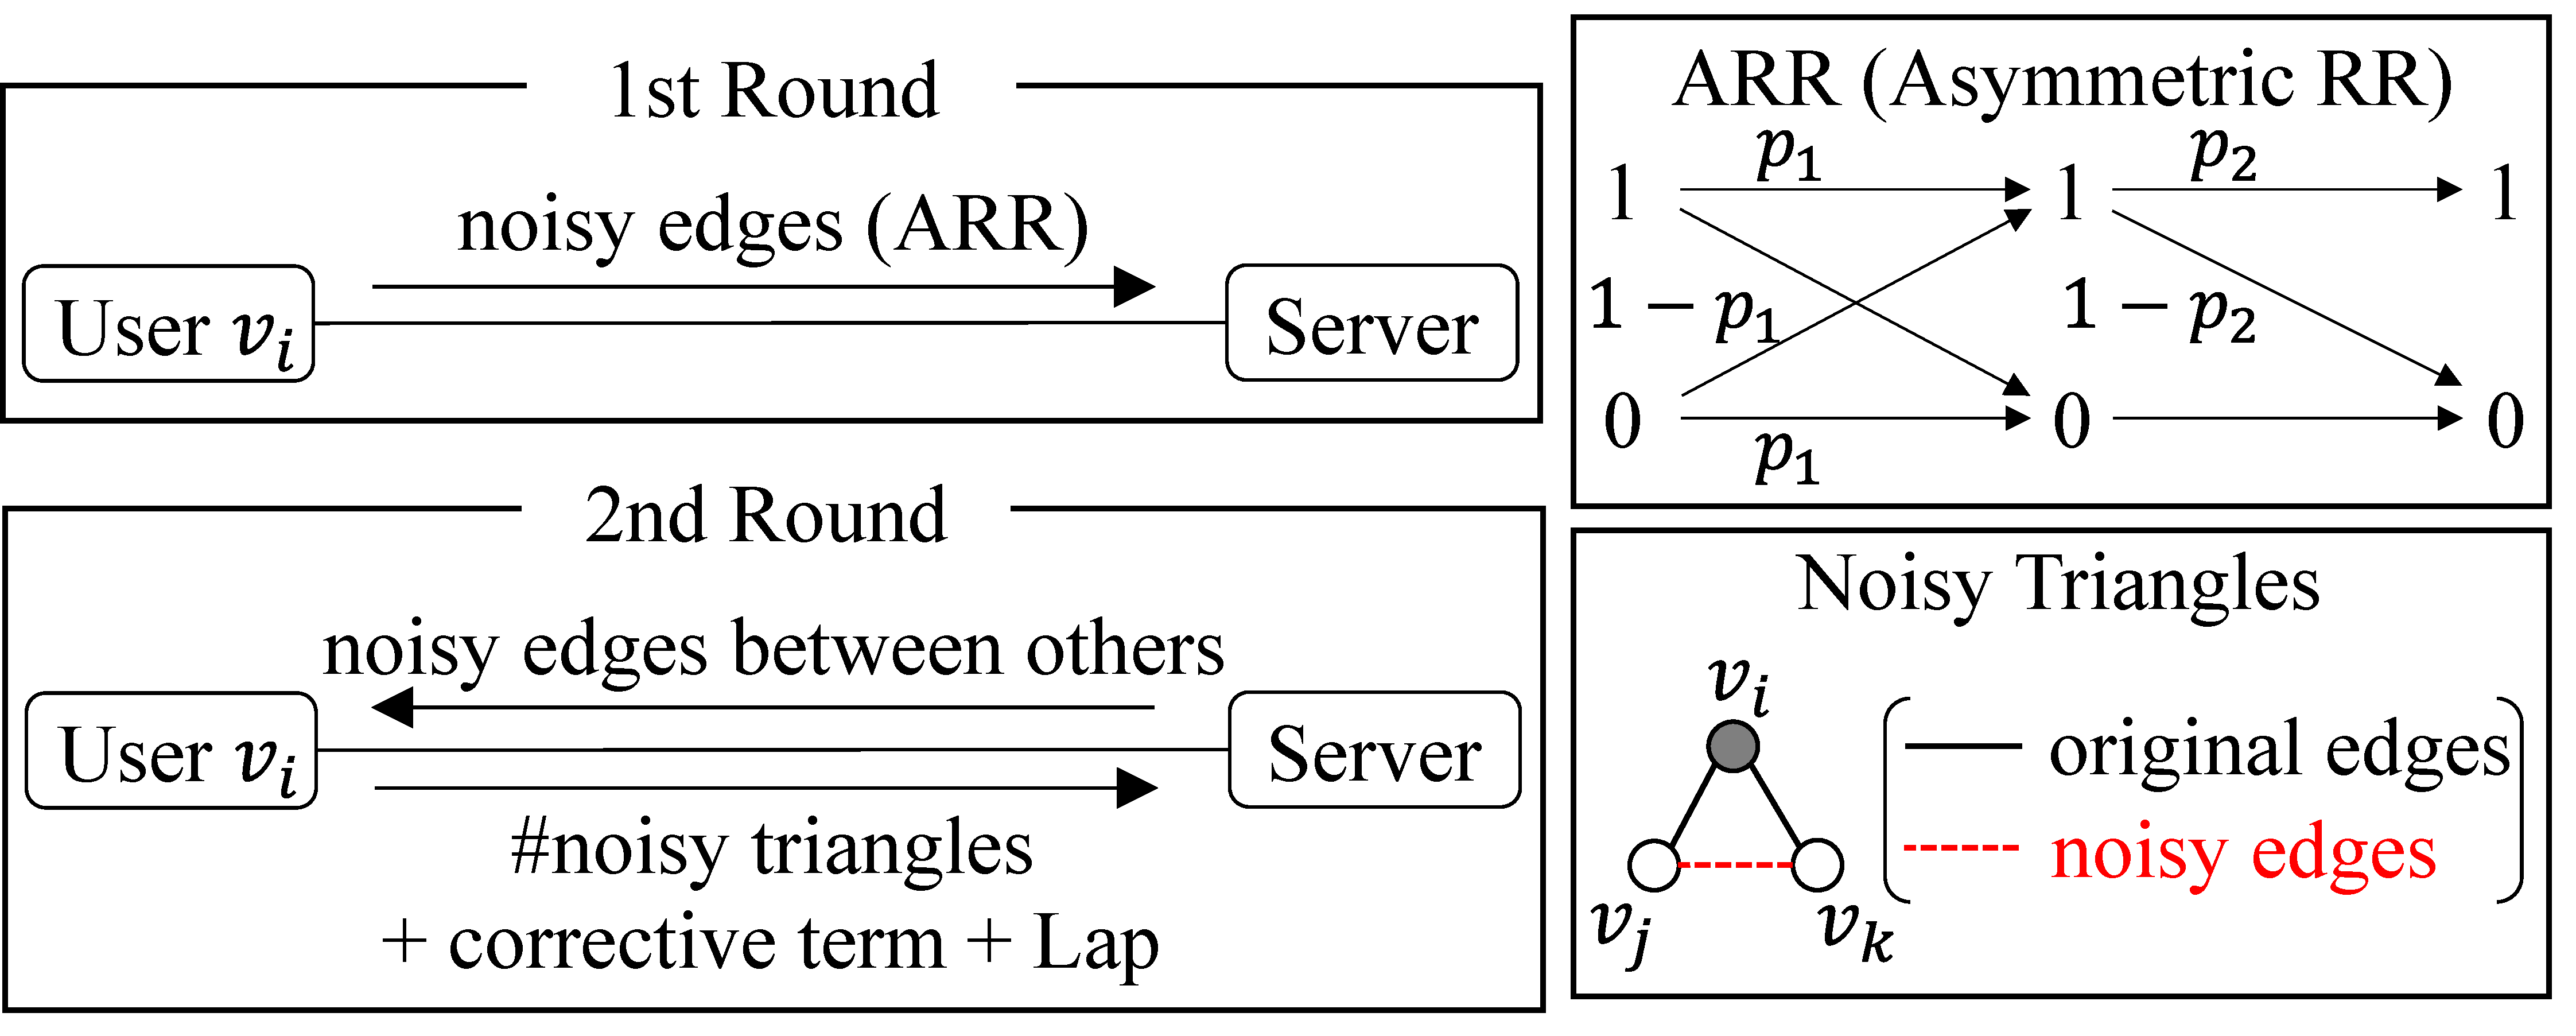
\includegraphics[width=0.99\linewidth]{fig/algorithm_overview.pdf}
  \vspace{-4mm}
  \caption{Overview of our communication-efficient triangle counting algorithms
  ($p_1 =\frac{e^{\epsilon}}{e^{\epsilon}+1}$,
  %$p_1 \in [\frac{1}{2},1]$,
  $p_2 \in [0,1]$).}
  %($\mu \in [0,1]$, $\rho = e^{-\epsilon_1}$).}
  %At the first round, each user obfuscates her edge by ARR ($\mu \in [0,1]$, $\rho \in e^{-\epsilon_1}$) to provide $\epsilon_1$-edge LDP.
  \label{chap2-fig:alg_overview}
\end{figure}

% \smallskip
% \noindent{\textbf{Our Two-Rounds Algorithms.}}~~
\smallskip
\noindent{\textbf{Algorithm Overview.}}~~Figure~\ref{chap2-fig:alg_overview} shows the overview of our proposed algorithms.
% all of which are run in two rounds.
% Below we explain the overview of our algorithms\footnote{For ease of explanation, we explain algorithms that use all elements in $\bmA$ in Section~\ref{chap2-sub:algorithms_overview}.
% In Section~\ref{chap2-sub:three_algorithms}, we propose algorithms that use only the lower triangular part of $\bmA$ to avoid the doubling issue, as described in Section~\ref{chap2-sub:LDP}.}.

At the first round, each user $v_i$ obfuscates
% $i-1$ bits for smaller user IDs in her neighbor list $\bma_i$ (i.e., lower triangular part of $\bmA$)
% each bit of her neighbor list $\bma_i$
% (for users with smaller user IDs)
bits for smaller user IDs in her neighbor list $\bma_i$
% (i.e., lower triangular part of $\bmA$)
by an LDP mechanism which we call the \textit{ARR (Asymmetric Randomized Response)} 
and sends the obfuscated bits to a server. 
% (note that we use only the lower triangular part of $\bmA$ to avoid the doubling issue, as described in Section~\ref{chap2-sub:LDP}).
The ARR is a combination of Warner's RR and edge sampling; i.e.,
we apply Warner's RR that outputs 1 or 0 as it is with probability
% $p_1\in[\frac{1}{2},1]$
$p_1$ ($=\frac{e^{\epsilon}}{e^{\epsilon}+1}$)
and then sample each 1 with probability $p_2\in[0,1]$.
%
% Given 1 (resp.~0) as input, the ARR outputs 1 with probability $\mu$ (resp.~$\mu\rho$), where $\mu \in [0,1]$, $\rho = e^{-\epsilon_1}$, and $\epsilon_1 \in \nnreals$.
% We can view this mechanism as a combination of Warner's RR~\cite{Warner_JASA65} and edge sampling; i.e., we apply Warner's RR that
% outputs 1 or 0 as it is with probability $p_1=\frac{e^{\epsilon_1}}{e^{\epsilon_1}+1}$
% and then sample each 1 with probability $p_2\in[0,1]$, where $\mu=p_1 p_2$.
% In fact, the ARR with $\mu = p_1$ (i.e., $p_2=1$) is equivalent to Warner's RR.
Unlike Warner's RR, the ARR is asymmetric in that the flip probability in the whole process is different
depending on the input value.
As with Warner's RR, the ARR provides edge LDP.
% Since Warner's RR provides
% $\epsilon_1$-
% edge LDP (as described in Section~\ref{chap2-sub:LDP}) and
% the sampling is a post-processing process (and
% DP is immune to post-processing~\cite{DP}, the ARR also provides
% $\epsilon_1$-
% edge LDP.
We can also significantly reduce the number of 1s (hence the communication cost) by setting
% the sampling probability
$p_2$ small.
% $\mu$ much smaller than $p_1$.
% Let $E' \subseteq V \times V$ be a set of noisy edges sent by users.

At the second round, the server calculates a message $M_i$ for user $v_i$ consisting of some or all noisy edges between others. 
We propose three strategies for calculating $M_i$. 
% and
% each user
User $v_i$ downloads $M_i$ from the server.
% a message $M_i$ from the server consisting of some or all
% of $E'$.
% noisy edges between others.
Then, since user $v_i$ knows her edges, $v_i$ can count \textit{noisy triangles} ($v_i$, $v_j$, $v_k$) such that $j<k<i$ and only one edge ($v_j$, $v_k$) is noisy, as shown in Figure~\ref{chap2-fig:alg_overview}. 
% $(v_i,v_j) \in E$, $(v_i,v_k) \in E$,
% $(v_j,v_k) \in E'$, and $j<k<i$;
% i.e., only one edge is noisy
The condition $j<k<i$ is imposed to use only the lower triangular part of $\bmA$, i.e., 
to avoid the doubling issue in Section~\ref{chap2-sub:LDP}. 
% Then $v_i$ adds some post-processing (to enable the server to obtain an unbiased estimate of $f_\triangle(G)$) and the Laplacian noise (to provide $\epsilon_2$-edge LDP for $\epsilon_2 \in \nnreals$) to the noisy triangle count, and sends it to a server.
User $v_i$ adds %some post-processing
a corrective term
%(to enable the server to obtain an unbiased estimate of $f_\triangle(G)$) 
and the Laplacian noise
% (to provide edge LDP)
to the noisy triangle count 
and sends it to a server.
The corrective term is added to enable the server to obtain an unbiased estimate of $f_\triangle(G)$. 
The Laplacian noise provides
% $\epsilon_2$-
edge LDP.
% , where $\epsilon_2 \in \nnreals$.
% From this,
Finally,
the server calculates an unbiased estimate of $f_\triangle(G)$
from the noisy data sent by users.
By composition (Proposition~\ref{chap2-prop:seq_comp_edge_LDP}),
% the compositionality of DP~\cite{DP},
our algorithms provide
% ($\epsilon_1 + \epsilon_2$)-
edge LDP in total.

\smallskip
\noindent{\textbf{Remark.}}~~Note that it is also possible for the server to calculate an unbiased estimate of $f_\triangle(G)$ at the first round.
However, this results in a
prohibitively
% very
large estimation error
% for a large graph
% for two reasons.
because
% First,
all edges sent by users are noisy; i.e., three edges are noisy in any triangle.
% all three edges are noisy in any triangle at the first round (whereas only one edge is noisy in our algorithms),
% Second, the noisy graph is dense, and consequently the time complexity of counting noisy triangles is $O(n^3)$. Thus, some approximation (such as edge sampling) is necessary to efficiently compute the estimate of $f_\triangle(G)$.
In contrast, only one edge is noisy in each noisy triangle at the second round because each user $v_i$ knows two original edges
% $(v_i,v_j) \in E$ and $(v_i,v_k) \in E$
connected to $v_i$.
Consequently, we can obtain an unbiased estimate with a much smaller variance.
See Appendix~\ref{chap2-sec:one-round} for a detailed comparison.
% In Appendix~\ref{chap2-sec:one-round}, we show that
% our two-rounds algorithms significantly outperform the existing one-round triangle algorithms.
% ~\cite{Imola_USENIX21,Ye_TKDE21}.
% (with sampling).
% the estimation error is significantly reduced by introducing an additional round.

% \subsection{Three Algorithms}
\subsection{Algorithms}
\label{chap2-sub:three_algorithms}

\smallskip
\noindent{\textbf{ARR.}}~~First, we formally define the ARR.
% We begin with a formal definition of the ARR.
% Below we describe our algorithms in detail.
The ARR has two parameters: $\epsilon \in \nnreals$ and $\mu \in [0,\frac{e^{\epsilon}}{e^{\epsilon} + 1}]$.
The parameter $\epsilon$ is the privacy budget, and $\mu$ controls the communication cost.

Let
% $\calR_{ARR}$
$ARR_{\epsilon,\mu}$ be the ARR with parameters $\epsilon$ and $\mu$. It takes $0/1$ as input and outputs $0/1$ with the following probability:
\begin{align}
    \Pr[ARR_{\epsilon,\mu}(1) = b] &= \begin{cases}\mu & (b=1) \\ 1-\mu & (b=0)\end{cases} \label{chap2-eq:ARR_1}\\
    \Pr[ARR_{\epsilon,\mu}(0) = b] &= \begin{cases}\mu\rho & (b=1) \\ 1-\mu \rho & (b=0), \end{cases} \label{chap2-eq:ARR_0}
\end{align}
where $\rho = e^{-\epsilon}$.
By Figure~\ref{chap2-fig:alg_overview},
we can view this randomizer as a combination of Warner's RR~\cite{Warner_JASA65}
% with $p_1=\frac{e^{\epsilon}}{e^{\epsilon}+1}$
and edge sampling, where $\mu=p_1 p_2$.
In fact, the ARR with $\mu = p_1 =\frac{e^{\epsilon}}{e^{\epsilon}+1}$ (i.e., $p_2=1$) is equivalent to Warner's RR.

Each user $v_i$ applies the ARR to bits for smaller user IDs in her neighbor list $\bma_i$; i.e., $\calR_i(\bma_i) = (ARR_{\epsilon,\mu}(a_{i,1}), \ldots, \allowbreak ARR_{\epsilon,\mu}(a_{i,i-1}))$.
% Note that we use only the lower triangular part of $\bmA$ to avoid the doubling issue described in Section~\ref{chap2-sub:LDP}.
Then $v_i$ sends $\calR_i(\bma_i)$ to the server.
% Applying Warner's RR to each bit of $\bma_i$ provides $\epsilon$-edge LDP (as described in Section~\ref{chap2-sub:LDP}).
Since applying Warner's RR to $\bma_i$ provides $\epsilon$-edge LDP (as described in Section~\ref{chap2-sub:LDP}) and the sampling is a post-processing process, applying the ARR to $\bma_i$ also provides $\epsilon$-edge LDP by the immunity to post-processing~\cite{DP}.

Let $E' \subseteq V \times V$ be a set of noisy edges sent by users.

\smallskip
\noindent{\textbf{Which Noisy Edges to Download?}}~~Now, the main question
tackled in this paper is: \textit{Which noisy edges should each user $v_i$
download at the second round?}
Note that
% user $v_i$ cannot leak her original edges to the server.
% For example,
user $v_i$
% cannot
is not allowed to
download only a set of noisy edges that form noisy triangles
(i.e., $\{(v_j,v_k) \in E' | (v_i,v_j) \in E, (v_i,v_k) \in E$\}),
% a set of noisy edges $\{(v_j,v_k) \in E' | (v_i,v_j) \in E, (v_i,v_k) \in E$\} (i.e., only noisy edges that form noisy triangles),
because it tells the server
% the fact that $v_j$ and $v_k$ are friends with $v_i$.
who are friends with $v_i$.
In other words, user $v_i$ cannot leak her original edges to the server when she
downloads noisy edges; the server must choose which part of $E'$ to include in
the message $M_i$ it sends her.

Thus, a natural solution would be to download \textit{all noisy edges between others}
% (except for the ones connected to $v_i$).
(with smaller user IDs); i.e.,
% \begin{align}
% M_i =\{(v_j, v_k) \in E' | j<k<i\}. \label{chap2-eq:M_i_I}
% \end{align}
$M_i =\{(v_j, v_k) \in E' | j<k<i\}$.
% as shown in Figure~\ref{chap2-fig:noisy_edge_DL}.
We denote our algorithm with this full download strategy by \AlgOne{}.
The (inefficient) two-rounds algorithm in~\cite{Imola_USENIX21} is a special case of \AlgOne{}
without sampling ($\mu = p_1$).
% when $\mu = p_1$ (i.e., when we
% use Warner's RR and
% do not sample edges).
In other words, \AlgOne{} is a generalization of the two-rounds algorithm in~\cite{Imola_USENIX21} using the ARR.
% $(v_j,v_k) \in E'$ such that $(v_i,v_j) \in E$, $(v_i,v_k) \in E$
% The expected download size in \AlgOne{} is $O(\mu n^2)$.

% Since users have already sent noisy edges at the first round, user $v_i$ can use noisy edges connected to $v_i$ when downloading noisy edges.
% For example,

In this paper,
we show that we can do much better
% we achieve much higher utility
than \AlgOne{}.
Specifically, we prove in Section~\ref{chap2-sub:algorithms_theoretical_analysis} that \AlgOne{} results in a high estimation error when the number of 4-cycles (cycles of length 4) in $G$ is large.
Intuitively, this can be explained as follows.
Suppose that $v_i$, $v_j$, $v_{i'}$, and $v_k$
($j<k<i$, $j<k<i'$)
form a 4-cycle. 
% $v_i-v_j-v_{i'}-v_k-v_i$.
% (denoted by $v_i$-$v_j$-$v_{i'}$-$v_k$).
% , as shown in the left panel of Figure~\ref{chap2-fig:four-cycle}.
There is no triangle in this graph.
However, if there is a noisy edge between $v_j$ and $v_k$, then two (incorrect) noisy triangles appear: ($v_i$, $v_j$, $v_k$) counted by $v_i$ and ($v_{i'}$, $v_j$, $v_k$) counted by $v_{i'}$.
More generally, let $E_{ijk}$ (resp.~$E_{i'jk}$) $\in \{0,1\}$ be a random variable that takes $1$ if ($v_i$, $v_j$, $v_k$) (resp.~($v_{i'}$, $v_j$, $v_k$)) forms a noisy triangle and $0$ otherwise.
Then, the covariance $\cov(E_{ijk},E_{i'jk})$ between $E_{ijk}$ and $E_{i'jk}$ is large because the presence/absence of a single noisy edge ($v_j$, $v_k$) affects the two noisy triangles.

To address this issue, we introduce a
% \textit{trick}
trick 
% trick, which we call the ``$4$-cycle trick'',
that makes the two noisy triangles \textit{less correlated with each other}.
We call this the \textit{4-cycle trick}.
% Since users have already sent noisy edges at the first round,
% user $v_i$ can use noisy edges connected to $v_i$ when downloading noisy edges.
Specifically,
% we propose two algorithms: \AlgTwo{} and \AlgThree{}.
we propose two algorithms in which
% user $v_i$ uses noisy edges connected to $v_i$ when downloading noisy edges.
the server uses noisy edges connected to $v_i$ when it calculates a message $M_i$ for $v_i$.
In the first algorithm,
% user $v_i$ downloads
the server selects
noisy edges $(v_j, v_k)$ such that
one noisy edge is connected from $v_k$ to $v_i$;
% there is a noisy edge between $v_i$ and $v_k$;
i.e.,
$M_i = \{(v_j, v_k) \in E' | (v_i, v_k) \in E', j<k<i\}$.
% \begin{align}
% M_i = \{(v_j, v_k) \in E' | (v_i, v_k) \in E', j<k<i\}. \label{chap2-eq:M_i_II}
% \end{align}
We call this algorithm \AlgTwo{}, as one noisy edge is connected to $v_i$.
In the second algorithm,
% user $v_i$ downloads
the server selects
noisy edges $(v_j, v_k)$ such that
two noisy edges are connected from these nodes to $v_i$; i.e.,
$M_i = \{(v_j, v_k) \in E' | (v_i, v_j) \in E', (v_i, v_k) \in E', j<k<i\}$.
% \begin{align}
% \hspace{-2mm} M_i \hspace{-0.5mm} = \hspace{-0.5mm}  \{(v_j, v_k) \in E' | (v_i, v_j) \in E', (v_i, v_k) \in E', j<k<i\}. \label{chap2-eq:M_i_III}
% \end{align}
We call this algorithm \AlgThree{}, as two noisy edges are connected to $v_i$.
Note that user $v_i$ does not leak her original edges to the server at the time of download in these algorithms, because
% $v_i$ uses only noisy edges the server has.
the server uses only noisy edges $E'$ sent by users to calculate $M_i$.

Figure~\ref{chap2-fig:noisy_edge_DL} shows our three algorithms.
% Let $\mu_F, \mu_O, \mu_T \in \nnreals$ be values of $\mu$ in the ARR used for \AlgOne{}, \AlgTwo{}, and \AlgThree{}, respectively.
% Then the
The download cost $\CostDL{}$ in (\ref{chap2-eq:cost_DL}) is
$O(\mu n^2 \log n)$, $O(\mu^2 n^2 \log n)$, and $O(\mu^3 n^2 \log n)$,
% $O(\mu_F n^2 \log n)$, $O(\mu_O^2 n^2 \log n)$, and $O(\mu_T^3 n^2 \log n)$,
respectively, when we regard $\epsilon$ as a constant.
In our experiments, we set
the parameter $\mu$ in the ARR so that
% $\mu$ in \AlgOne{}, $\mu^2$ in \AlgTwo{}, and $\mu^3$ in \AlgThree{} are equal
$\mu$ in \AlgOne{} is equal to $\mu^2$ in \AlgTwo{} and also equal to $\mu^3$ in \AlgThree{};
e.g., $\mu=10^{-6}$, $10^{-3}$, and $10^{-2}$ in \AlgOne{}, \AlgTwo{}, and \AlgThree{}, respectively.
% $\mu_F$, $\mu_O$, and $\mu_T$ to $\mu_F = \mu_O^2 = \mu_T^3$ (e.g., $\mu_F=10^{-6}$, $\mu_O=10^{-3}$, $\mu_T=10^{-2}$)
% so that
% the expected download size
Then
the download cost
is the same between the three algorithms.

\begin{figure}[t]
  \centering
  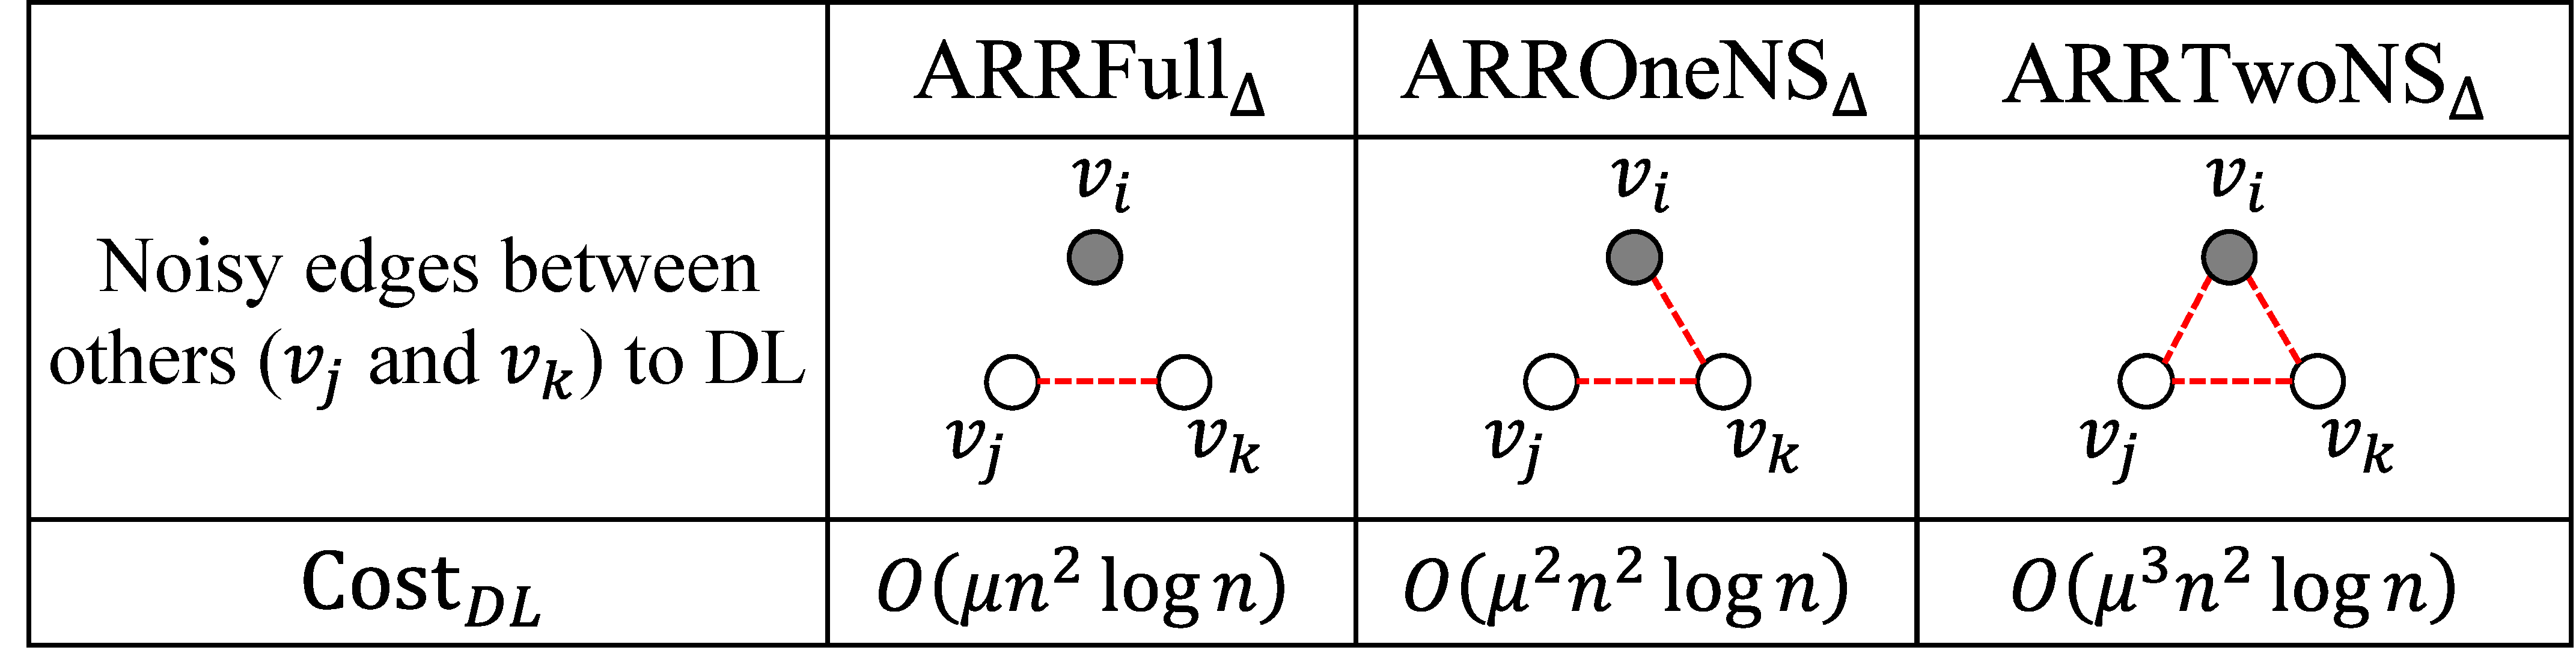
\includegraphics[width=0.99\linewidth]{fig/three_algorithms.pdf}
  \vspace{-4mm}
  \caption{Noisy edges to download
  % and expected download size
  in our three algorithms.}
  %$\mu_F$, $\mu_O$, and $\mu_T$ are values of $\mu$ in the ARR used for \AlgOne{}, \AlgTwo{}, and \AlgThree{}, respectively.}
  \label{chap2-fig:noisy_edge_DL}
% \end{figure}
\vspace{4mm}
% \begin{figure}[t]
  \centering
  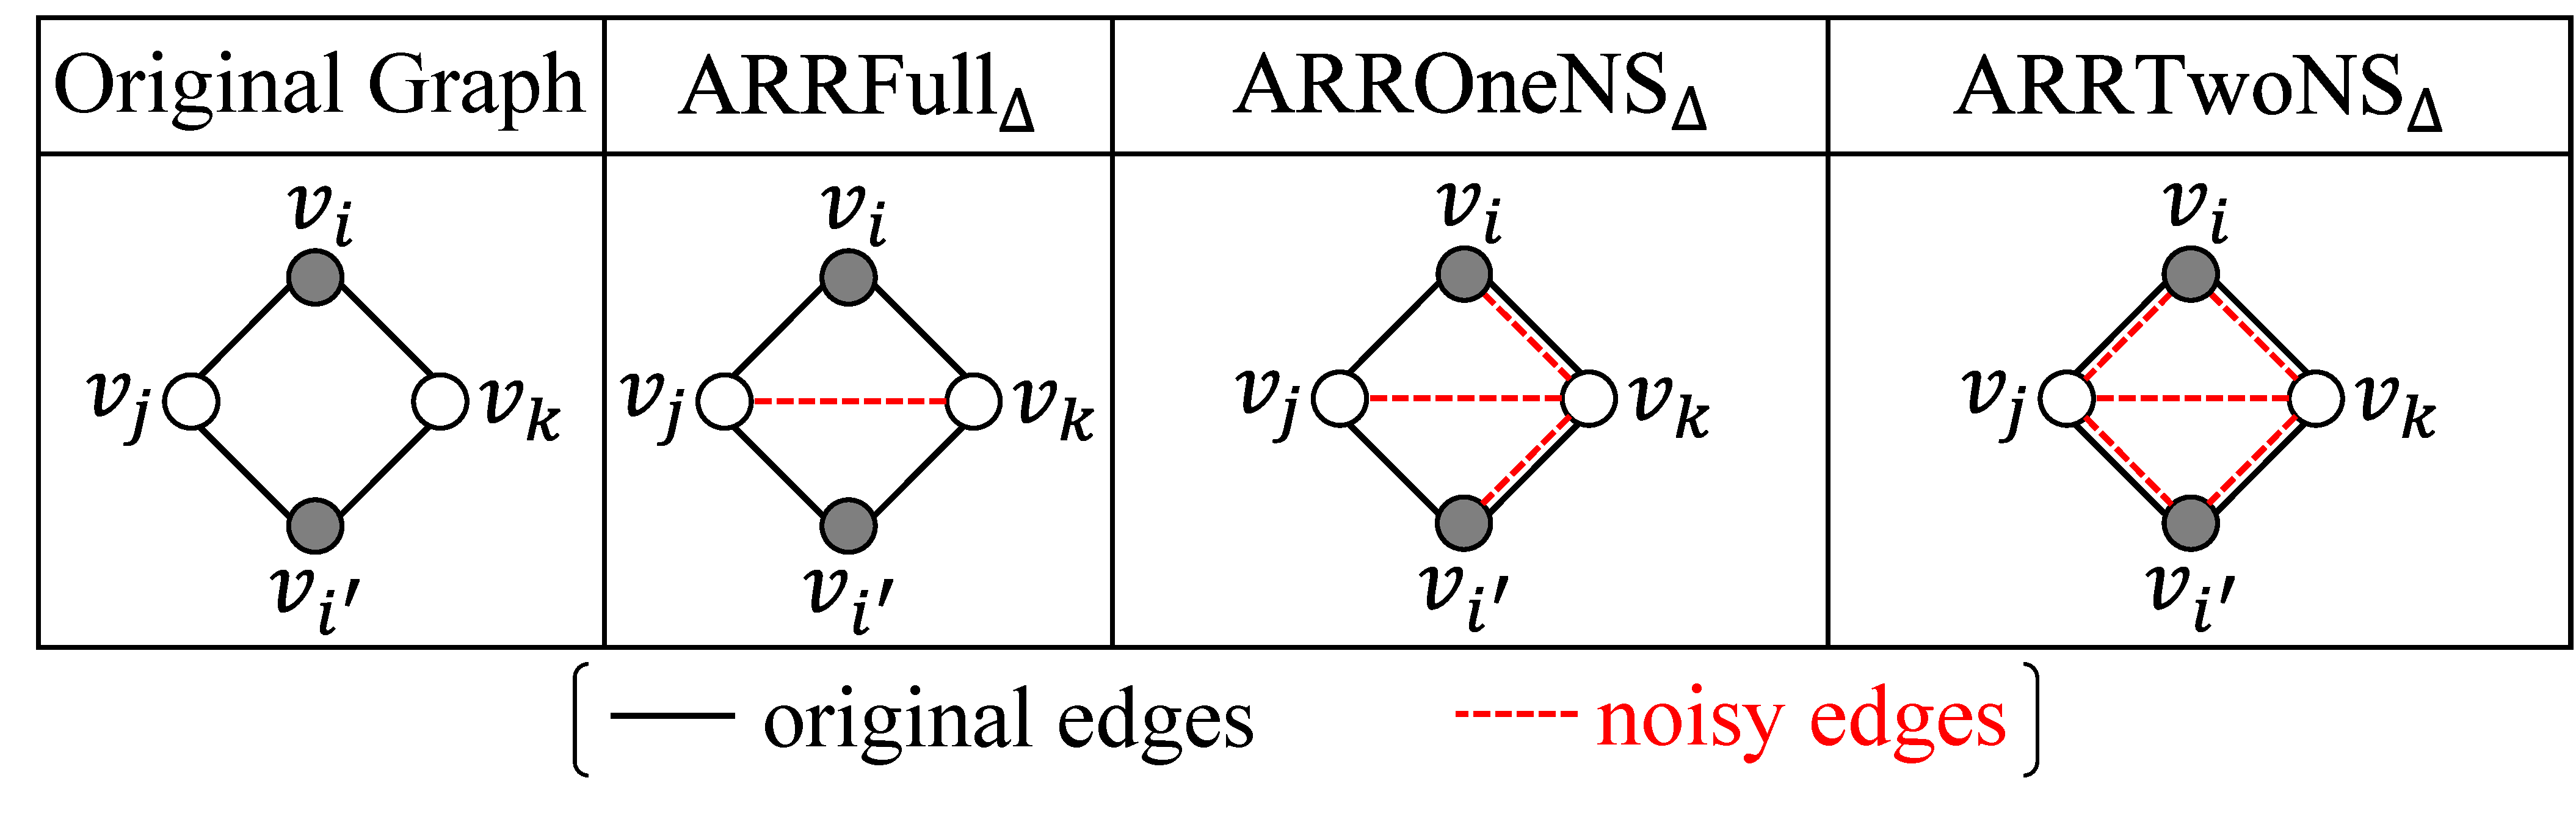
\includegraphics[width=0.95\linewidth]{fig/four_cycle.pdf}
  \vspace{-4mm}
  \caption{4-cycle trick.
  % 4-cycle issue.
  \AlgOne{} counts two (incorrect) noisy triangles when one noisy edge appears.
  \AlgTwo{} and \AlgThree{} avoid this by increasing independent noise.}
  \label{chap2-fig:four-cycle}
\end{figure}

% Figure\ref{chap2-fig:four-cycle} shows why and how \AlgTwo{} and \AlgThree{} address the 4-cycle issue.
Figure~\ref{chap2-fig:four-cycle} shows our $4$-cycle trick.
\AlgOne{} counts two (incorrect) noisy triangles when a noisy edge ($v_j$, $v_k$) appears.
% there is a noisy edge ($v_j$, $v_k$).
In contrast,
% the two noisy triangles are counted
\AlgTwo{} (resp.~\AlgThree{}) counts both the two noisy triangles
% this bad event happens
only when three (resp.~five) independent noisy edges appear,
% in \AlgTwo{} (resp.~\AlgThree{}),
as shown in Figure~\ref{chap2-fig:four-cycle}.
% Since these noisy edges are independent,
Thus, this bad event happens with a much smaller probability.
For example,
% when $\mu_F=10^{-6}$, $\mu_O=10^{-3}$, and $\mu_T=10^{-2}$,
% \AlgOne{}, \AlgTwo{}, and \AlgThree{} count both the two noisy triangles with probability $10^{-6}$, $10^{-9}$, and $10^{-10}$, respectively.
\AlgOne{} ($\mu=10^{-6}$),
\AlgTwo{} ($\mu=10^{-3}$), and
\AlgThree{} ($\mu=10^{-2}$)
count both the two noisy triangles with probability $10^{-6}$, $10^{-9}$, and $10^{-10}$, respectively.
The covariance $\cov(E_{ijk},E_{i'jk})$ of \AlgTwo{} and \AlgThree{} is also much smaller than that of \AlgOne{}.
% \AlgTwo{} and \AlgThree{} also achieve much smaller covariance $\cov(E_{ijk},E_{i'jk})$ than \AlgOne{}.


In our experiments, we show that \AlgTwo{} and \AlgThree{} significantly outperforms \AlgOne{}
% in two real graph datasets with a large number of 4-cycles.
for a large-scale graph or dense graph, in both of which
% when
the number of 4-cycles in $G$ 
% can be very 
is 
large.
% \ji{Are there other scenarios where the performance is better?}
% \commentT{I think the number of 4-cycles can be large when a graph is (i) large or (ii) dense (in particular, (i) is important). I clarified this.}

\smallskip
\noindent{\textbf{\AlgTwo{} vs. \AlgThree{}.}}~~One
% The number of independent noisy edges in a 4-cycle is three and five in \AlgTwo{} and \AlgThree{}, respectively, as shown in Figure\ref{chap2-fig:four-cycle}.
% Thus
might expect that \AlgThree{} outperforms \AlgTwo{} because \AlgThree{} addresses the 4-cycle issue more aggressively; i.e.,
% \AlgThree{} has the largest number of independent noisy edges in a 4-cycle,
the number of independent noisy edges in a 4-cycle is larger in \AlgThree{},
as shown in Figure \ref{chap2-fig:four-cycle}.
However,
% \AlgThree{} suffers from a large global sensitivity of the Laplacian noise at the second round.
\AlgTwo{} can reduce the global sensitivity of the Laplacian noise
at the second round
more effectively than \AlgThree{}, as explained in Section~\ref{chap2-sec:double_clip}.
% in detail.
Consequently, \AlgTwo{}, which is the most tricky algorithm, achieves the smallest estimation error in our experiments.
See Sections~\ref{chap2-sec:double_clip} and \ref{chap2-sec:experiments} for details of the global sensitivity and experiments, respectively.

\smallskip
\noindent{\textbf{Three Algorithms.}}~~Below we explain the details of our three algorithms.
For ease of explanation, we assume that the maximum degree $d_{max}$ is public in Section~\ref{chap2-sub:three_algorithms}\footnote{For example, $d_{max}$ is public in Facebook: $d_{max} = 5000$~\cite{Facebook_Limit}.
If the server does not have prior knowledge about $d_{max}$, she can privately estimate $d_{max}$ and use graph projection to guarantee that each user's degree never exceeds the private estimate of $d_{max}$~\cite{Imola_USENIX21}.
In any case, the assumption in Section~\ref{chap2-sub:three_algorithms} does not undermine our algorithms, because our entire algorithms with double clipping in Section~\ref{chap2-sec:double_clip} does \textit{not} assume that $d_{max}$ is public.}.
Note, however, that
% we propose a technique to significantly reduce the global sensitivity
our double clipping (which is proposed to significantly reduce the global sensitivity) in Section~\ref{chap2-sec:double_clip} does \textit{not} assume that $d_{max}$ is public.
Consequently, our entire algorithms 
% (i.e., \AlgOne, \AlgTwo, \AlgThree with double clipping)
% three triangle counting algorithms (\AlgOne, \AlgTwo, \AlgThree) with our double clipping
do \textit{not} require the assumption that $d_{max}$ is public.

\setlength{\algomargin}{5mm}
\begin{algorithm}[t]
  \SetAlgoLined
  \KwData{Graph $G \in \calG$ represented as neighbor lists $\bma_1, \ldots, \bma_n
    \in \{0,1\}^n$, privacy budgets
  $\epsilon_1,\epsilon_2 \in \nnreals$, $d_{max} \in \nnints$,
  $\mu \in [0,\frac{e^{\epsilon_1}}{e^{\epsilon_1} + 1}]$.
  %$\mu^*$.
  }
  \KwResult{Private estimate $\hf_\triangle(G)$ of $f_\triangle(G)$.}
%   $p_1 \leftarrow \frac{1}{e^{\epsilon_1}}$\;
  [s] $\rho \leftarrow e^{-\epsilon_1}$\;
  [$v_i$, s] $\mu^* \leftarrow \mu$, $\mu^2$, and $\mu^3$ in F, O, and T, respectively\;
  \tcc{First round.}
  \For{$i=1$ \KwTo $n$}{
    [$v_i$] $\bmr_i \leftarrow (ARR_{\epsilon_1,\mu}(a_{i,1}), \ldots,
    ARR_{\epsilon_1,\mu}(a_{i,i-1}))$\;
    [$v_i$] Upload $\bmr_i = (r_{i,1}, \ldots, r_{i,i-1})$ to the server\;
  }
%   $E' = \{(v_i, v_j) : i > j, r_{i,j} = 1\} \cup \{(v_j, v_i) : i > j, r_{i,j} =
%   1\}$\;
  [s] $E' = \{(v_j, v_k) :r_{k,j} = 1, j < k\}$\;
  \tcc{Second round.}
  \For{$i=1$ \KwTo $n$}{
    [s] Compute
    $M_i$ by (\ref{chap2-eq:M_i_I}), (\ref{chap2-eq:M_i_II}), and (\ref{chap2-eq:M_i_III}) in F, O, and T, respectively\;
    %$M_i = \{(v_j,v_k) \in E': j < k < i\}$\;
    %$M_i = \{(v_j,v_k) \in E': (v_i,v_k) \in E', j < k < i\}$\;
    %$M_i = \{(v_j,v_k) \in E': (v_i,v_k), (v_j,v_k) \in E', j < k < i\}$\;
    [$v_i$] Download $M_i$ from the server\;
    [$v_i$] $t_i \leftarrow |\{(v_i,v_j,v_k) :
    a_{i,j} = a_{i,k} = 1, (v_j,v_k) \in M_i, j<k<i \}|$\;
    [$v_i$] $s_i \leftarrow |\{(v_i,v_j,v_k) :
    a_{i,j} = a_{i,k} = 1, j<k<i\}|$\;
    [$v_i$] $w_i \leftarrow t_i - \mu^* \rho s_i$\;
    [$v_i$] $\hw_i \leftarrow w_i + \Lap(\frac{d_{max}}{\epsilon_2})$\;
    [$v_i$] Upload $\hw_i$ to the server\;
  }
  [s] $\hf_\triangle(G) \leftarrow \frac{1}{\mu^*(1-\rho)}\sum_{i=1}^n \hw_i$\;
  \KwRet{$\hf_\triangle(G)$}
  \caption{Our three algorithms.
  ``F'', ``O'', ``T'' are shorthands for
  %$\mu^*=\mu_F$, $\mu_O^2$, and $\mu_T^3$ in
  \AlgOne{}, \AlgTwo{}, and \AlgThree{}, respectively.
  [$v_i$] and [s] represent that the process is run by $v_i$ and the server, respectively.
  }\label{chap2-alg:unify}
\end{algorithm}

% As explained above,
Recall that the server calculates a message $M_i$ for $v_i$ as:
\begin{align}
\hspace{-1mm} M_i \hspace{-0.5mm} &= \hspace{-0.5mm} \{(v_j, v_k) \in E' | j<k<i\} \label{chap2-eq:M_i_I}\\
\hspace{-1mm} M_i \hspace{-0.5mm} &= \hspace{-0.5mm} \{(v_j, v_k) \in E' | (v_i, v_k) \in E', j<k<i\} \label{chap2-eq:M_i_II}\\
\hspace{-1mm} M_i \hspace{-0.5mm} &= \hspace{-0.5mm}  \{(v_j, v_k) \in E' | (v_i, v_j) \in E', (v_i, v_k) \in E', j<k<i\} \label{chap2-eq:M_i_III}
\end{align}
in \AlgOne{}, \AlgTwo{}, \AlgThree{}, respectively.

%Using these equations,
% our three algorithms can be unified in Algorithm~\ref{chap2-alg:unify}.
Algorithm~\ref{chap2-alg:unify} shows our three algorithms.
These algorithms are processed differently in lines 2 and 9; ``F'', ``O'', ``T'' are shorthands for \AlgOne{}, \AlgTwo{}, and \AlgThree{}, respectively.
% It uses two rounds of private computation, and
% in both rounds each user $v_i$ applies a local randomizer to her neighbor list $\bma_i$.
The privacy budgets for the first and second
rounds are $\epsilon_1, \epsilon_2 \in \nnreals$, respectively.

The first round appears in lines 3-7 of Algorithm~\ref{chap2-alg:unify}.
In this round, each user applies
$ARR_{\epsilon_1, \mu}$
% the ARR
defined by (\ref{chap2-eq:ARR_1}) and (\ref{chap2-eq:ARR_0}) to bits $a_{i,1}, \ldots, a_{i,i-1}$ for smaller user IDs in her neighbor list $\bma_i$, i.e., lower triangular part of $\bmA$.
% explained in the beginning of
% Section~\ref{chap2-sub:three_algorithms}.
Let $\bmr_i = (r_{i,1}, \ldots, r_{i,i-1}) \in \{0,1\}^{i-1}$ be the obfuscated bits of $v_i$.
User $v_i$ uploads $\bmr_i$ to the server.
Then the server combines the noisy edges together, forming $E' = \{(v_j, v_k) : r_{k,j} = 1, j < k\}$.

The second round appears in lines 8-17 of Algorithm~\ref{chap2-alg:unify}.
In this round, the server computes a message $M_i$
by (\ref{chap2-eq:M_i_I}), (\ref{chap2-eq:M_i_II}), or (\ref{chap2-eq:M_i_III}),
% depending on the algorithm,
and user $v_i$ downloads it.
% As explained above, \AlgOne{}, \AlgTwo{}, and \AlgThree{} computes $M_i$ by (\ref{chap2-eq:M_i_I}), (\ref{chap2-eq:M_i_II}), and  (\ref{chap2-eq:M_i_III}), respectively.
Then user $v_i$ calculates the number $t_i \in \nnints$ of noisy triangles ($v_i$, $v_j$, $v_k$) such that
% $j<k<i$ and
only one edge ($v_j$, $v_k$) is noisy, as shown in Figure~\ref{chap2-fig:alg_overview}.
% involving two edges in user $v_i$'s neighbor list and one noisy edge in $E'$ (as shown in Figure~\ref{chap2-fig:alg_overview}).
% We also emphasize that the condition $j<k<i$ is imposed to use only the lower triangular part of $\bmA$.
% (and avoid the doubling issue).
User $v_i$ also calculate a corrective term $s_i \in \nnints$.
The corrective term $s_i$ is the number of
possible triangles involving $v_i$ 
% that can be formed from edges in $v_i$'s neighbor list,
and is computed to obtain an unbiased estimate of $f_\triangle(G)$.
% unbias the triangle count.
User $v_i$ calculates $w_i = t_i - \mu^* \rho s_i$, where $\rho = e^{-\epsilon_1}$ and
% $\mu^* = \mu_F$, $\mu_O^2$, and $\mu_T^3$
$\mu^* = \mu$, $\mu^2$, and $\mu^3$
in ``F'', ``O'', and ``T'', respectively.
% \AlgOne{}, \AlgTwo{}, and \AlgThree{}, respectively.
Then $v_i$ adds the Laplacian noise $\Lap(\frac{d_{max}}{\epsilon_2})$ to $w_i$ to provide $\epsilon_2$-edge LDP and sends the noisy value $\hw_i$ ($= w_i + \Lap(\frac{d_{max}}{\epsilon_2})$) to the server. 
Note that adding one edge increases both $t_i$ and $s_i$ 
% results in the increase of the triangle count 
by at most $d_{max}$. 
Thus, the global sensitivity of $w_i$ is at most $d_{max}$. 
Finally, the server calculates an estimate of $f_\triangle(G)$ as: $\hf_\triangle(G) = \frac{1}{\mu^*(1-\rho)}\sum_{i=1}^n \hw_i$.
As we prove later, $\hf_\triangle(G)$ is an unbiased estimate of $f_\triangle(G)$.

% \smallskip
% \noindent{\textbf{\AlgOne.}}

% Our first algorithm, \AlgOne, appears in Algorithm~\ref{chap2-alg:one}. It uses two
% rounds of private computation, and in both rounds each user applies a local
% randomizer to his data.
% The privacy budgets for the two
% rounds are $\epsilon_1, \epsilon_2$.

% The first round appears in Lines 3-4 of Algorithm~\ref{chap2-alg:one}. This round
% collects the noisy edges from the users.
% The noisy edges are produced
% using the asymmetric randomized response mechanism, which we denote
% $ARR_{\epsilon, \mu}$. Recall that a bit $a_{i,j}$ of $\bma_i$ takes value $1$
% if and only if user $v_i$ includes user $v_j$ in his neighbor list. ARR is
% defined by $\Pr[ARR_{\epsilon, \mu}(1) = 1] = \mu$ and $\Pr[ARR_{\epsilon,
% \mu}(0) = 1] = \mu p_1$ where $p_1 = e^{-\epsilon_1}$. User $v_i$ uploads
% $\bmr_i$, the vector of ARR mechanisms applied to $a_{i,j}$ for $j < i$. This
% means that user $v_i$ ignores users with a bigger index than $i$. By doing so,
% for every possible undirected edge $(v_i, v_j)$, exactly one of $v_i, v_j$ will
% upload the
% edge using ARR. This prevents releasing the edge twice, and allows us to prove
% that our mechanism satisfies relationship DP without the doubling factor in
% $\epsilon$ (see Proposition~\ref{chap2-prop:edge_LDP_entire_edge_LDP}).
% Given the collection of ARR queries to the users, the server concludes the first
% round by combining the noisy edges together and unordering them, forming $E'$.

% The second round appears in Lines 8-13 of Algorithm~\ref{chap2-alg:one}.
% In this round, each user $v_i$ computes an unbiased estimator $w_i$ for
% the number of triangles involving $v_i$ for which the maximum index of the
% triangle is $i$. It is easy to see that the sum of the $w_i$ estimates the total
% number of triangles. The user does this by
% downloading the message $M = E'$ from the server
% and computing a noisy triangle count $t_i$ and a corrective term $s_i$. The count
% $t_i$ is the number of triangles involving two edges in user $v_i$'s neighbor
% list and one noisy edge in $E'$. The corrective term $s_i$ is the number of
% possible triangles that can be formed from edges in user $v_i$'s neighbor list,
% and is computed to unbias the triangle count. We emphasize that user $v_i$
% only considers the part of his neighbor list involving users of a lower index
% than $i$ for all calculations, including this. The unbiased estimator is
% given by $w_i = t_i - \mu_F p_1 s_i$---because it depends on the private data
% $\bma_i$, the user adds Laplacian noise of width $\frac{d_{max}}{\epsilon_2}$ to
% $w_i$ that the computation may satisfy $\epsilon_2$ edge LDP. He then uploads
% the noisy value $\hw_i$, and the server computes the final triangle estimate.

% \begin{algorithm}
%   \SetAlgoLined
%   \KwData{Graph $G$ represented as neighbor lists $\bma_1, \ldots, \bma_n
%     \in \{0,1\}^n$, two privacy budgets
%   $\epsilon_1,\epsilon_2 > 0$, $d_{max} \in \nnints$, sampling parameter
%   $\mu_F$.}
%   \KwResult{Private estimate of $f_\triangle(G)$.}
%   $p_1 \leftarrow \frac{1}{e^{\epsilon_1}}$\;
%   \tcc{First round.}
%   \For{$i=1$ \KwTo $n$}{
%     $\bmr_i \leftarrow (ARR_{\epsilon_1,\mu_F}(a_{i,1}), \ldots,
%     ARR_{\epsilon_1,\mu_F}(a_{i,i-1}))$\;
%     Upload $\bmr_i$ to server\;
%   }
%   $E' = \{(v_j, v_i) : i > j, r_{i,j} = 1\}$\;
%   \tcc{Second round.}
%   \For{$i=1$ \KwTo $n$}{
%     Server lets $M_i = E'$.
%     Download $M_i$ from server\;
%     $t_i \leftarrow |\{(v_i,v_j,v_k) :
%     j<k<i, a_{i,j} = a_{i,k} = 1, (k,j) \in M \}|$\;
%     $s_i \leftarrow |\{(v_i,v_j,v_k) :
%     j<k<i, a_{i,j} = a_{i,k} = 1\}|$\;
%     $w_i \leftarrow t_i - \mu_F p_1 s_i$\;
%     $\hw_i \leftarrow w_i + \Lap(\frac{d_{max}}{\epsilon_2})$\;
%     Upload $\hw_i$ to server\;
%   }
%   \KwRet{$\frac{1}{\mu_F(1-p_1)}\sum_{i=1}^n \hw_i$}
%   \caption{\AlgOne}\label{chap2-alg:one}
% \end{algorithm}

% \smallskip
% \noindent{\textbf{\AlgTwo.}}

% Our second Algorithm, \AlgTwo, appears in Algorithm~\ref{chap2-alg:two}. Like
% \AlgOne, it uses two rounds with budgets $\epsilon_1$ and $\epsilon_2$.
% The first round is identical to \AlgOne, and for brevity, Algorithm~\ref{chap2-alg:two} does not
% include a description of the first round.
% Recall that the goal of the second round is for each user $v_i$ to compute an estimate of the
% number of triangles in which $i$ is the maximum index, which is the variable
% $\hw_i$.
% The difference between \AlgOne and
% \AlgTwo is that in the second round of \AlgTwo (Lines 2-8), a user only downloads a
% subset of edges in
% $E'$: $v_i$ downloads those edges $(v_j, v_k) \in E'$ such that $j < k < i$ and
% $v_i \text{\----} v_k \text{\----} v_j$ are connected in $E'$. The server is
% able to compute these edges since they only depend on the first round release,
% and we denote it with $M_i$. User $v_i$ then computes his estimate $w_i = t_i -
% \mu_O^2 p_1 s_i$, where $t_i$ is and $s_i$ are the same quantities as in
% \AlgOne. The final estimator $w_i = t_i - \mu_O^2
% p_1 s_i$ is an unbiased estimate of the number of triangles for which $i$ is the
% maximum index. User $v_i$ uploads $\hw_i$, given by $w_i$ plus Laplace noise, in
% order to share $w_i$ privately.

% Downloading only some of $E'$, depending on the noisy first round, actually
% produces a noisier estimator $\hw_i$ than \AlgOne. However, the communication
% cost of \AlgTwo is less, precisely because a subset of $E'$ is downloaded. It
% is straightforward to prove that in expectation, user $v_i$ downloads $\mu_F
% n^2$ edges in \AlgOne and $\mu_O^2 n^2$ edges in \AlgTwo. Thus, the two
% algorithms have comparable communication when $\mu_F = \mu_O^2$, meaning that
% $\mu_F \ll \mu_O$. Thus, \AlgOne is forced to sample edges at a much smaller
% ratio than \AlgTwo in the first round, producing a much noisier value of $E'$.
% At these two different sampling ratios, the estimator $\hw_i$ in \AlgTwo is not
% necessarily worse than the same estimator in \AlgOne

% \begin{algorithm}
%   \SetAlgoLined
%   \KwData{Graph $G$ represented as neighbor lists $\bma_1, \ldots, \bma_n
%     \in \{0,1\}^n$, two privacy budgets
%   $\epsilon_1,\epsilon_2 > 0$, $d_{max} \in \nnints$, sampling parameter
%   $\mu_O$.}
%   \KwResult{Private estimate of $f_\triangle(G)$.}
%   \tcc{Second round.}
%   \For{$i=1$ \KwTo $n$}{
%     Server computes $M_i = \{(j,k) : j < k < i, (k,i), (j,k) \in E'\}$\;
%     Download $M_i$ from server\;
%     $t_i \leftarrow |\{(v_i,v_j,v_k) :
%     j<k<i, a_{i,j} = a_{i,k} = 1, (j,k) \in M_i\}|$\;
%     $s_i \leftarrow |\{(v_i,v_j,v_k) :
%     j<k<i, a_{i,j} = a_{i,k} = 1\}|$\;
%     $w_i \leftarrow t_i - \mu_O^2 p_1 s_i$\;
%     $\hw_i \leftarrow w_i + \Lap(\frac{d_{max}}{\epsilon_2})$\;
%     Upload $\hw_i$ to server\;
%   }
%   \KwRet{$\frac{1}{\mu_O^2(1-p_1)}\sum_{i=1}^n \hw_i$}
%   \caption{\AlgTwo, second round only (first round is identical to \AlgOne with
%   sampling parameter $\mu_O$).}\label{chap2-alg:two}
% \end{algorithm}

% \smallskip
% \noindent{\textbf{\AlgThree.}}~~TBD
% \colorB{\begin{itemize}
%     \item Algorithm of \AlgThree (only the 2nd round).
% \end{itemize}}

% \begin{algorithm}
%   \SetAlgoLined
%   \KwData{Graph $G$ represented as neighbor lists $\bma_1, \ldots, \bma_n
%     \in \{0,1\}^n$, two privacy budgets
%   $\epsilon_1,\epsilon_2 > 0$, $d_{max} \in \nnints$, sampling parameter
%   $\mu_T$.}
%   \KwResult{Private estimate of $f_\triangle(G)$.}
%   \tcc{Second round.}
%   \For{$i=1$ \KwTo $n$}{
%     Server computes $M_i = \{(j,k) : j < k < i, (k,i), (j,k), (j,i) \in E'\}$\;
%     Download $M_i$ from server\;
%     $t_i \leftarrow |\{(v_i,v_j,v_k) :
%     j<k<i, a_{i,j} = a_{i,k} = 1, (j,k) \in M_i \}|$\;
%     $s_i \leftarrow |\{(v_i,v_j,v_k) :
%     j<k<i, a_{i,j} = a_{i,k} = 1\}|$\;
%     $w_i \leftarrow t_i - \mu_T^3 p_1 s_i$\;
%     $\hw_i \leftarrow w_i + \Lap(\frac{d_{max}}{\epsilon_2})$\;
%     Upload $\hw_i$ to server\;
%   }
%   \KwRet{$\frac{1}{\mu_T^3(1-p_1)}\sum_{i=1}^n \hw_i$}
%   \caption{\AlgThree, second round only (first round is identical to \AlgOne
%   with sampling parameter $\mu_T$).}\label{chap2-alg:three}
% \end{algorithm}

% \smallskip
% \noindent{\textbf{Summary.}}~~TBD
% \colorB{\begin{itemize}
%     \item One algorithm table unifying all three algorithms (e.g., $\mu^* = \mu_F$, $\mu_o^2$, $\mu_T^3$ in \AlgOne, \AlgTwo, and \AlgThree, respectively).
% \end{itemize}}

\subsection{Theoretical Analysis}
\label{chap2-sub:algorithms_theoretical_analysis}
We now introduce the theoretical guarantees on
% theoretically analyze
the privacy, communication, and
utility of 
our algorithms. 
% \AlgOne{}, \AlgTwo{}, and \AlgThree{}.
% All the proofs appear in Appendix~\ref{chap2-sec:proof_algorithms}.
% The first round of the
% algorithms is all the same: Each user applies a randomizer $\calR_i^1(\bma_i)$
% to his neighbor list which releases the ARR of his neighbors. Then, the server
% computes $M_i$ in a different way depending on the algorithm.
% Let $M_i^F, M_i^O,
% M_i^T$ be the message $M_i$ used in \AlgOne{}, \AlgTwo{}, and \AlgThree{}, respectively.
% Formulas for these values appear in
% equations~\eqref{chap2-eq:M_i_I},~\eqref{chap2-eq:M_i_II}, and~\eqref{chap2-eq:M_i_III},
% respectively.
% For fixed $M_i$ and $\mu^*$, the second round of the algorithms is
% also the same, and we denote it with $\calR_i^{2}(M_i, \mu^*)(\bma_i)$, where $\mu^* =
% \mu, \mu^2, \mu^3$ depending on \AlgOne{}, \AlgTwo{}, or \AlgThree{}. Notice
% that the final triangle estimate $\hf_\triangle(G)$ is given by a post-processing of
% $\{\calR_i^2(M_i, \mu^*)(\bma_i) : 1 \leq i \leq n\}$.

% \paragraph{Privacy}
\smallskip
\noindent{\textbf{Privacy.}}~~We first show the privacy guarantees:
% The privacy guarantee of our three algorithms comes from proving that
% $\calR_i^1(\bma_i)$ and $\calR_i^2(M_i, \mu^*)(\bma_i)$ satisfies $\epsilon$-edge DP for any choice of $M_i, \mu^*$,
% they satisfy $\epsilon_1$ and $\epsilon_2$-edge LDP at the first and second round, respectively,
% $\epsilon$-edge DP for any choice of $M_i, \mu^*$,
% and then using sequential composition (Proposition~\ref{chap2-prop:seq_comp_edge_LDP}):
% and post-processing:
\begin{theorem}\label{chap2-thm:privacy_algorithms}
  % Let $\mu, d_{max}$ be fixed.
  For $i \in [n]$,
  let
%   $\calR_i^1, \calR_i^2(M_i, \mu^*)$
  $\calR_i^1, \calR_i^2(M_i)$
  be the randomizers used by user $v_i$ in
  rounds $1$ and $2$ of Algorithm~\ref{chap2-alg:unify}. % where $M_i = M_i^F, M_i^O$, or $M_i^T$.
  Let
%   $\calR_i(\bma_i) = (\calR_i^1(\bma_i), \calR_i^2(M_i, \mu^*)(\bma_i))$
  $\calR_i(\bma_i) = (\calR_i^1(\bma_i), \calR_i^2(M_i)(\bma_i))$
  be the composition of the two randomizers. Then,
  $\calR_i$
%   $\calR_i$ satisfies $(\epsilon_1 + \epsilon_2)$-edge LDP for $i \in [n]$, and $(\calR_1,
%   \ldots, \calR_n)$ satisfies $(\epsilon_1 + \epsilon_2)$-relationship DP.
%   Thus, by post-processing, the output of Algorithm~\ref{chap2-alg:unify}
  satisfies
  $(\epsilon_1+\epsilon_2)$-edge LDP and
  $(\calR_1,
  \ldots, \calR_n)$ satisfies  $(\epsilon_1+\epsilon_2)$-relationship DP.
\end{theorem}

% A full proof of this claim appears in Appendix~\ref{chap2-sec:proof_algorithms}.
% The algorithms satisfy both $(\epsilon_1+\epsilon_2)$-edge LDP and $(\epsilon_1+\epsilon_2)$-relationship DP
Note that the doubling issue in Section~\ref{chap2-sub:LDP} does not occur, 
because we use only the lower triangular part of $\bmA$. 
% (i.e., avoid the doubling issue in Section~\ref{chap2-sub:LDP}).
% each user ignores edges in her neighbor list to users with smaller index than his own.
% Thus, each edge affects the output of at most one randomizer in
% each round. This allows us to prove a tighter bound on the relationship DP
% parameter than that given by Proposition~\ref{chap2-prop:edge_LDP_entire_edge_LDP}.
By the immunity to post-processing, the estimate  $\hf_\triangle(G)$
% in Algorithm~\ref{chap2-alg:unify}
also satisfies $(\epsilon_1+\epsilon_2)$-edge LDP and $(\epsilon_1+\epsilon_2)$-relationship DP.

% \paragraph{Communication}
\smallskip
\noindent{\textbf{Communication.}}~~Recall that we evaluate the algorithms based on their download cost~\eqref{chap2-eq:cost_DL} and upload cost~\eqref{chap2-eq:cost_UL}.

\textit{Download Cost:} The download cost is the number of bits required
to download $M_i$.
% Each user can represent $M_i$
$M_i$ can be represented
as
% pairs of edges, which
a list of edges between others, and each edge
can be
identified with two indices (user IDs), i.e., $2 \log n$ bits.
% Thus, the total communication is $2 (\log n)\E[|M_i|]$.
% The number of edges in $M_i$ depends on \AlgOne{}, \AlgTwo{}, and \AlgThree{}.
There are $\frac{(n-1)(n-2)}{2} \approx \frac{n^2}{2}$ edges between others.
% Given 1 (resp.~0) as input, $ARR_{\epsilon_1,\mu}$ outputs 1 with probability $\mu$ (resp.~$\mu e^{- \epsilon_1}$).
$ARR_{\epsilon_1,\mu}$ outputs 1 with probability at most $\mu$. 
% When $d_{max} \ll n$, most input values are 0.
In addition, each noisy triangle must have $1$, $2$, and $3$ noisy edges in \AlgOne{}, \AlgTwo{}, and \AlgThree{}, respectively, as shown in Figure~\ref{chap2-fig:noisy_edge_DL}.

Thus, 
% when $d_{max} \ll n$, 
the download cost in Algorithm~\ref{chap2-alg:unify} 
% for each algorithm 
can be written as:
% ($F$, $O$, and $T$ are shorthands for \AlgOne{}, \AlgTwo{}, and \AlgThree{}, respectively):
% Notice that any element $(v_j, v_k)$ is included independently in $E'$ with
% probability at most $\mu$. Any element $(v_j, v_k)$ appears in $M_i^F$ (resp. $M_i^O$, $M_i^T$)
% if and only if $1$ (resp. $2,3$) other elements appears in $E'$. Thus, the
% probability an element appears in $M_i^F$ (resp. $M_i^O, M_i^T$) is at most
% $\mu$ (resp. $\mu^2, \mu^3$).
% Hence, $\E[|M_i^F|] \leq \mu \binom{n}{2}$, $\E[|M_i^O|] \leq \mu^2 \binom{n}{2}$,
% and $\E[|M_i^F|] \leq \mu^3 \binom{n}{2}$. In summary, we have (where $F,O,T$ is a
% shorthand for \AlgOne{}, \AlgTwo{}, and \AlgThree{}),
\begin{align}
   Cost_{DL} &\leq \mu^* n^2 \log n,  \label{chap2-eq:CostDL_F}
%   Cost_{DL}(F) &\leq \mu n^2 \log n,  \label{chap2-eq:CostDL_F}\\
%   Cost_{DL}(O) &\leq \mu^2 n^2 \log n \label{chap2-eq:CostDL_O}\\
%   Cost_{DL}(T) &\leq \mu^3 n^2 \log n. \label{chap2-eq:CostDL_T}
%   Cost_{DL}(F) &\leq \mu n^2 \log n \label{chap2-eq:CostDL_F}\\
%   Cost_{DL}(O) &\leq \mu^2 n^2 \log n \label{chap2-eq:CostDL_O}\\
%   Cost_{DL}(T) &\leq \mu^3 n^2 \log n. \label{chap2-eq:CostDL_T}
%   Cost_{DL}(F) &\approx \mu e^{-\epsilon_1} n^2 \log n \label{chap2-eq:CostDL_F}\\
%   Cost_{DL}(O) &\approx \mu^2 e^{-\epsilon_1} n^2 \log n \nonumber\\
%   Cost_{DL}(T) &\approx \mu^3 e^{-\epsilon_1} n^2 \log n. \nonumber
%   Cost_{DL}(F) &= \max_{i=1}^n 2(\log n) \E[|M_i^F|] \leq \mu n^2 \log n \\
%   Cost_{DL}(O) &= \max_{i=1}^n 2(\log n) \E[|M_i^O|] \leq \mu^2 n^2 \log n \\
%   Cost_{DL}(T) &= \max_{i=1}^n 2(\log n) \E[|M_i^T|] \leq \mu^3 n^2 \log n
\end{align}
where $\mu^* = \mu$, $\mu^2$, and $\mu^3$ in \AlgOne{}, \AlgTwo{}, and \AlgThree{}, respectively. 
In (\ref{chap2-eq:CostDL_F}), 
% (\ref{chap2-eq:CostDL_O}), and (\ref{chap2-eq:CostDL_T}), 
we upper-bounded $\CostDL{}$ by using the fact that $ARR_{\epsilon_1,\mu}$ outputs 1 with probability at most $\mu$. 
However, when $d_{max} \ll n$, 
$ARR_{\epsilon_1,\mu}$ outputs 1 with probability $\mu e^{- \epsilon_1}$ in most cases. 
In that case, we can roughly approximate $\CostDL{}$ by replacing $\mu$ with $\mu e^{- \epsilon_1}$ in (\ref{chap2-eq:CostDL_F}). 
% , (\ref{chap2-eq:CostDL_O}), and (\ref{chap2-eq:CostDL_T}). 
% In our experiments, we also confirmed that this approximation is accurate up to three significant digits.

\textit{Upload Cost:}
% For each of the three algorithms,
The upload cost comes
from the number of bits required to upload $\calR_i^1(\bma_i)$ and
% $\calR_i^2(M_i, \mu^*)(\bma_i)$.
$\calR_i^2(M_i)(\bma_i)$.
Uploading $\calR_i^1(\bma_i)$ involves uploading
$\bmr_i$ (line 5), which is a list of up to $n$ noisy neighbors. By sending just
the indices (user IDs) of the $1$s in $\bmr_i$, each user sends $\|\bmr_i\|_1 \log n$ bits,
where $\|\bmr_i\|_1$ is the number of 1s in $\bmr_i$.
% (note that $\log n$ bits are required to express each index).
When we use $ARR_{\epsilon_1,\mu}$,
% defined by (\ref{chap2-eq:ARR_1}) and (\ref{chap2-eq:ARR_0}),
we have $\E[\|\bmr_i\|_1] \leq \mu n$.
% since the probability of any bit of $\bmr_i$ is
% at most $\mu$.
% Moreover, $\E[\|\bmr_i\|_1] \approx \mu e^{-\epsilon_1} n$ when $d_{max} \ll n$.
% for a sparse graph where each bit in the original graph $G$ is $0$ in most cases.
% 
% For any choice of $M_i, \mu^*$,
Uploading
% $\calR_i^2(M_i, \mu^*)$
$\calR_i^2(M_i)$
involves uploading a single real number $\hw_i$ (line 15), which is negligibly small (e.g., 64 bits when we use a double-precision floating-point).
% While it is
% theoretically possible for $\hw_i$ to
% have arbitrarily large magnitude due to the Laplace noise, $\hw_i$ can be
% clipped and rounded so that it can be sent accurately with $O(\log n)$ bits. We
% do not provide a theoretical analysis of how to do this because the upload cost of
% the first round is much higher.

Thus,
% when $d_{max} \ll n$, 
the upload cost in Algorithm~\ref{chap2-alg:unify} can be written as:
% approximated as:
% for each of the three algorithms, we have
%
\begin{align}
%   Cost_{UL} = \max_{i=1}^n \E[\|\bmr_i\|_1]\log n + \E[bits(\hw_i)] = O(\mu n \log n).
%   Cost_{UL} \approx \mu e^{- \epsilon_1} n \log n.
  Cost_{UL} \leq \mu n \log n.
% \]
\label{chap2-eq:CostUL_proposal}
\end{align}
% where $\mu$ is $\mu_F$, $\mu_O$, and $\mu_T$ in \AlgOne{}, \AlgTwo{}, and \AlgThree{}, respectively.
Clearly, 
% the upload cost 
$\CostUL{}$ 
is much smaller than 
% the download cost 
$\CostDL{}$ 
for large $n$.

% \paragraph{Utility}
\smallskip
\noindent{\textbf{Utility.}}~~Analyzing the expected $l_2$ loss $l_2^2(f_\triangle(G), \hf_\triangle(G))$ of the algorithms involves first proving that
the estimator $\hf_\triangle$ is unbiased
% (i.e., for any graph $G$, $\E[\hf_\triangle(G)] = f_\triangle(G)$)
and then
% . Then, we
% control
analyzing
the
variance $\V[\hf_\triangle(G)]$ to obtain an upper-bound on
$l_2^2(f_\triangle(G), \hf_\triangle(G))$.
This is given in the following:

\begin{theorem}\label{chap2-thm:l2loss_algorithms}
  %Let $G, \mu, \epsilon$ be fixed.
  Let $G \in \calG$, $\epsilon_1, \epsilon_2 \in \nnreals$, and
  $\mu \in [0,\frac{e^{\epsilon_1}}{e^{\epsilon_1} + 1}]$.
%   $\mu_F, \mu_O, \mu_T \in [0,\frac{e^{\epsilon}}{e^{\epsilon_1} + 1}]$.
  %Let $G$, $\mu_F$, $\mu_O$, and $\mu_T$ be fixed.
  Let $\hf_\triangle^F(G), \hf_\triangle^O(G)$,
  and $\hf_\triangle^T(G)$ be
  the
  % estimators returned
  estimates output
  respectively by \AlgOne{}, \AlgTwo{}, and \AlgThree{} in Algorithm~\ref{chap2-alg:unify}.
  %, respectively.
  Then, $\E[\hf_\triangle^F(G)] = \E[\hf_\triangle^O(G)] = \E[\hf_\triangle^T(G)] = f_\triangle(G)$ (i.e., estimates are unbiased) and
   %Furthermore,
   %when no Laplace noise is added (i.e. $\epsilon_2 = \infty$),
   %we have:
   \begin{align*}
      l_2^2(f_\triangle(G), \hf_\triangle^F(G)) &\leq \textstyle{\frac{2C_4(G)+S_2(G)}{\mu(1-e^{\epsilon_1})^2} + \frac{2nd_{max}^2}{\mu^2(1-e^{\epsilon_1})^2\epsilon_2^2}} \\
      l_2^2(f_\triangle(G), \hf_\triangle^O(G)) &\leq \textstyle{\frac{\mu(2 C_4(G) + 6S_3(G)) + S_2(G)}{\mu^2(1-e^{\epsilon_1})^2} \hspace{-0.5mm}+\hspace{-0.5mm} \frac{2nd_{max}^2}{\mu^4(1-e^{\epsilon_1})^2\epsilon_2^2}}\\
      l_2^2(f_\triangle(G), \hf_\triangle^T(G)) &\leq \textstyle{\frac{\mu^2(2 C_4(G) + 6S_3(G)) + S_2(G)}{\mu^3(1-e^{\epsilon_1})^2} \hspace{-0.5mm}+\hspace{-0.5mm} \frac{2nd_{max}^2}{\mu^6(1-e^{\epsilon_1})^2\epsilon_2^2},}
   \end{align*}
   where $C_4(G)$ is the number of $4$-cycles in $G$
   %$P_3(G)$ is the number of $3$-paths in $G$,
   and $S_k(G)$ is the number of $k$-stars in $G$. %(see Figure~\ref{chap2-fig:subgraphs} in Appendix~\ref{chap2-sec:notations_subgraphs} for their shapes).
   %For a general $\epsilon_2$, the above quantities increase by an additive factor of
   %$2n \left(\frac{d_{max}}{\mu^*(1-e^{\epsilon_1})\epsilon_2}\right)^2$.
\end{theorem}
For each of the three upper-bounds in Theorem~\ref{chap2-thm:l2loss_algorithms}, the first and second terms are the estimation errors caused by empirical estimation and the Laplacian noise, respectively.
We also note that
% $C_4(G) = P_3(G) = S_3(G) = O(n d_{max}^3)$
$C_4(G) = S_3(G) = O(n d_{max}^3)$
and $S_2(G) = O(n d_{max}^2)$.
% when we regard $\epsilon_1$ and $\epsilon_2$ as constants.
Thus, for small
% $\mu_F$ ($=\mu_O^2 = \mu_T^3$),
$\mu$,
the $l_2$ loss of empirical estimation can be expressed as $O(n d_{max}^3)$, $O(n d_{max}^2)$, and $O(n d_{max}^2)$ in \AlgOne{}, \AlgTwo{}, \AlgThree{}, respectively
% (when we regard $\epsilon_1$ as a constant),
% (as the factors of $S_3(G)$ and $P_3(G)$
% diminish for small $\mu$).
(as the factors of $C_4(G)$ and $S_3(G)$
diminish for small $\mu$).
% can be removed by $\mu$.
% The large $l_2$ loss of \AlgOne{} is caused by the number $C_4$ of $4$-cycles that is written as $O(n d_{max}^3)$.

This highlights our $4$-cycle trick.
The large $l_2$ loss of \AlgOne{} is caused by the number $C_4(G) = O(n d_{max}^3)$ of $4$-cycles.
\AlgTwo{} and \AlgThree{} addresses this issue by increasing independent noise, as shown in Figure~\ref{chap2-fig:four-cycle}.
% The theorem highlights the $4$-cycle issue of \AlgOne{}, because its utility guarantee depends on the number of $4$-cycles in $G$. While the number of $4$-cycles is strictly less than the number of $3$-paths, the other algorithms benefit from being able to set $\mu$ higher, and thus sample less.

% However,
% % all of our three algorithms still suffer from a very large estimation error. due to a large amount of the Laplacian noise.
% all of the upper-bounds in Theorem~\ref{chap2-thm:l2loss_algorithms} are still very large.
% % due to a large amount of the Laplacian noise (as shown in our experiments).
% % In particular,
% This is because
% the Laplacian noise is very large especially for small $\epsilon_2$ or
% % $\mu_F$ ($=\mu_O^2 = \mu_T^3$),
% $\mu$,
% as shown in Theorem~\ref{chap2-thm:l2loss_algorithms}.
% % In Section~\ref{chap2-sec:double_clip}, we introduce a double clipping technique to significantly reduce the amount of Laplacian noise.
% In
% % Section~\ref{chap2-sec:double_clip},
% the next section,
% we introduce \textit{double clipping} to significantly reduce the amount of Laplacian noise.

% our three algorithms

% \begin{figure}
%   \begin{tabular}{|l|l|l|l|}
%     \hline
%     & \AlgOne & \AlgTwo & \AlgThree \\ \hline
%     Privacy & $\epsilon_1 + \epsilon_2$ & $\epsilon_1 + \epsilon_2$ &
%     $\epsilon_1 + \epsilon_2$ \\ \hline
%     Utility & $\frac{1}{\mu_F(1-e^{-\epsilon_1})}O\left( \square(G) + \wedge(G)
%     + \frac{2nd_{max}^2}{\mu_F \epsilon_2^2}\right)$ & 0
%     & 0 \\ \hline
%     $\text{Cost}_{DL}$ & $\mu_F n^3 \log n$ & $\mu_O^2 n^3 \log n$ & $\mu_T^3
%     n^3 \log n$ \\ \hline
%     $\text{Cost}_{UL}$ & $\mu_Fn \log n$ & $\mu_O n \log n$ & $\mu_T n \log n$ \\ \hline
%   \end{tabular}
% \end{figure}

\section{Double Clipping}
\label{chap2-sec:double_clip}

% However, 
% all of our three algorithms still suffer from a very large estimation error. due to a large amount of the Laplacian noise. 
In Section~\ref{chap2-sec:algorithms}, 
% \ref{chap2-sub:algorithms_theoretical_analysis}, 
we showed that the estimation error caused by empirical estimation (i.e., the first term in Theorem~\ref{chap2-thm:l2loss_algorithms}) is significantly reduced by the $4$-cycle trick. 
However, 
% all of the upper-bounds in 
the estimation error is 
% caused by the Laplacian noise (i.e., the second term)  
% Theorem~\ref{chap2-thm:l2loss_algorithms} are 
still very large in our algorithms presented in Section~\ref{chap2-sec:algorithms}, as shown in our experiments. 
% due to a large amount of the Laplacian noise (as shown in our experiments). 
% In particular, 
This is because 
the estimation error by the Laplacian noise (i.e., the second term in Theorem~\ref{chap2-thm:l2loss_algorithms}) 
% the Laplacian noise 
is very large, especially for small $\epsilon_2$ or 
% $\mu_F$ ($=\mu_O^2 = \mu_T^3$), 
$\mu$. 
% as shown in Theorem~\ref{chap2-thm:l2loss_algorithms}. 
% In Section~\ref{chap2-sec:double_clip}, we introduce a double clipping technique to significantly reduce the amount of Laplacian noise.
This error term is tight and unavoidable as long as we use $d_{max}$ as a global sensitivity, which suggests that we need a better global sensitivity analysis.
% In 
% Section~\ref{chap2-sec:double_clip}, 
% the next section, 
% we introduce \textit{double clipping} to significantly reduce the amount of Laplacian noise.
% 
% Our three algorithms in Section~\ref{chap2-sec:algorithms} suffer from a large amount of the Laplacian noise. 
% due to the large global sensitivity. 
% To address this issue, 
% Thus, we propose a double clipping technique, which significantly reduces the global sensitivity of the Laplacian noise. 
To significantly reduce the global sensitivity, we propose a novel \textit{double clipping} technique. 
% Therefore, we propose a double clipping technique, which significantly reduces the global sensitivity of the Laplacian noise. 

We describe the overview and details of our double clipping in Sections~\ref{chap2-sub:clip_overview} and \ref{chap2-sub:algorithms}, respectively. 
Then we perform theoretical analysis in Section~\ref{chap2-sub:clip_theoretical_analysis}.

\subsection{Overview}
\label{chap2-sub:clip_overview}

% \smallskip
\noindent{\textbf{Motivation.}}~~Figure~\ref{chap2-fig:reduce_noisy_triangles} shows noisy triangles involving edge $(v_i,v_j)$ counted by user $v_i$ in our three algorithms. 
Our algorithms in Section~\ref{chap2-sec:algorithms} 
% (and the two-rounds algorithm in \cite{Imola_USENIX21}) 
use the fact that the number of such noisy triangles (hence the global sensitivity) is upper-bounded by the maximum degree $d_{max}$ because 
%user $v_i$'s degree is at most $d_{max}$). 
adding one edge increases the triangle count by at most $d_{max}$. 
Unfortunately, this upper-bound is too large, as shown in our experiments. 
% Although this is correct, we 

% Our basic idea is that we can 
In this paper, we 
significantly reduce this upper-bound by using the parameter $\mu$ in the ARR and user $v_i$'s degree $d_i \in \nnints$ for users with smaller IDs. 
For example, 
% we can expect that 
the number of noisy triangles involving $(v_i,v_j)$ in \AlgOne is 
expected to be around 
$\mu d_i$ 
% ($\mu \ll 1$, $d_i < d_{max}$) 
% with high probability (larger than $0.5$) 
because one noisy edge is included in each noisy triangle (as shown in Figure~\ref{chap2-fig:reduce_noisy_triangles}) and all noisy edges are independent. 
$\mu d_i$ is very small, especially when we set $\mu \ll 1$ to reduce the communication cost.  
% Similarly, the expected number of noisy triangles involving $(v_i,v_j)$ in \AlgTwo is $\mu_O^2 d_i$ because two independent noisy edges are in each noisy triangle (as in Figure~\ref{chap2-fig:reduce_noisy_triangles}).

However, we cannot directly use $\mu d_i$ as an upper-bound of the global sensitivity in \AlgOne for two reasons. 
First, $\mu d_i$ leaks the exact value of user $v_i$'s degree $d_i$ 
and 
% , hence 
violates edge LDP. 
% friendship information of $v_i$ (e.g., as an extreme example, $d_i=0$ reveals the fact that $v_i$ has no friends). 
Second, the number of noisy triangles involving $(v_i,v_j)$ exceeds $\mu d_i$ with high probability (about $0.5$). 
Thus, the noisy triangle count cannot be upper-bounded by $\mu d_i$. 

\begin{figure}[t]
  \centering
  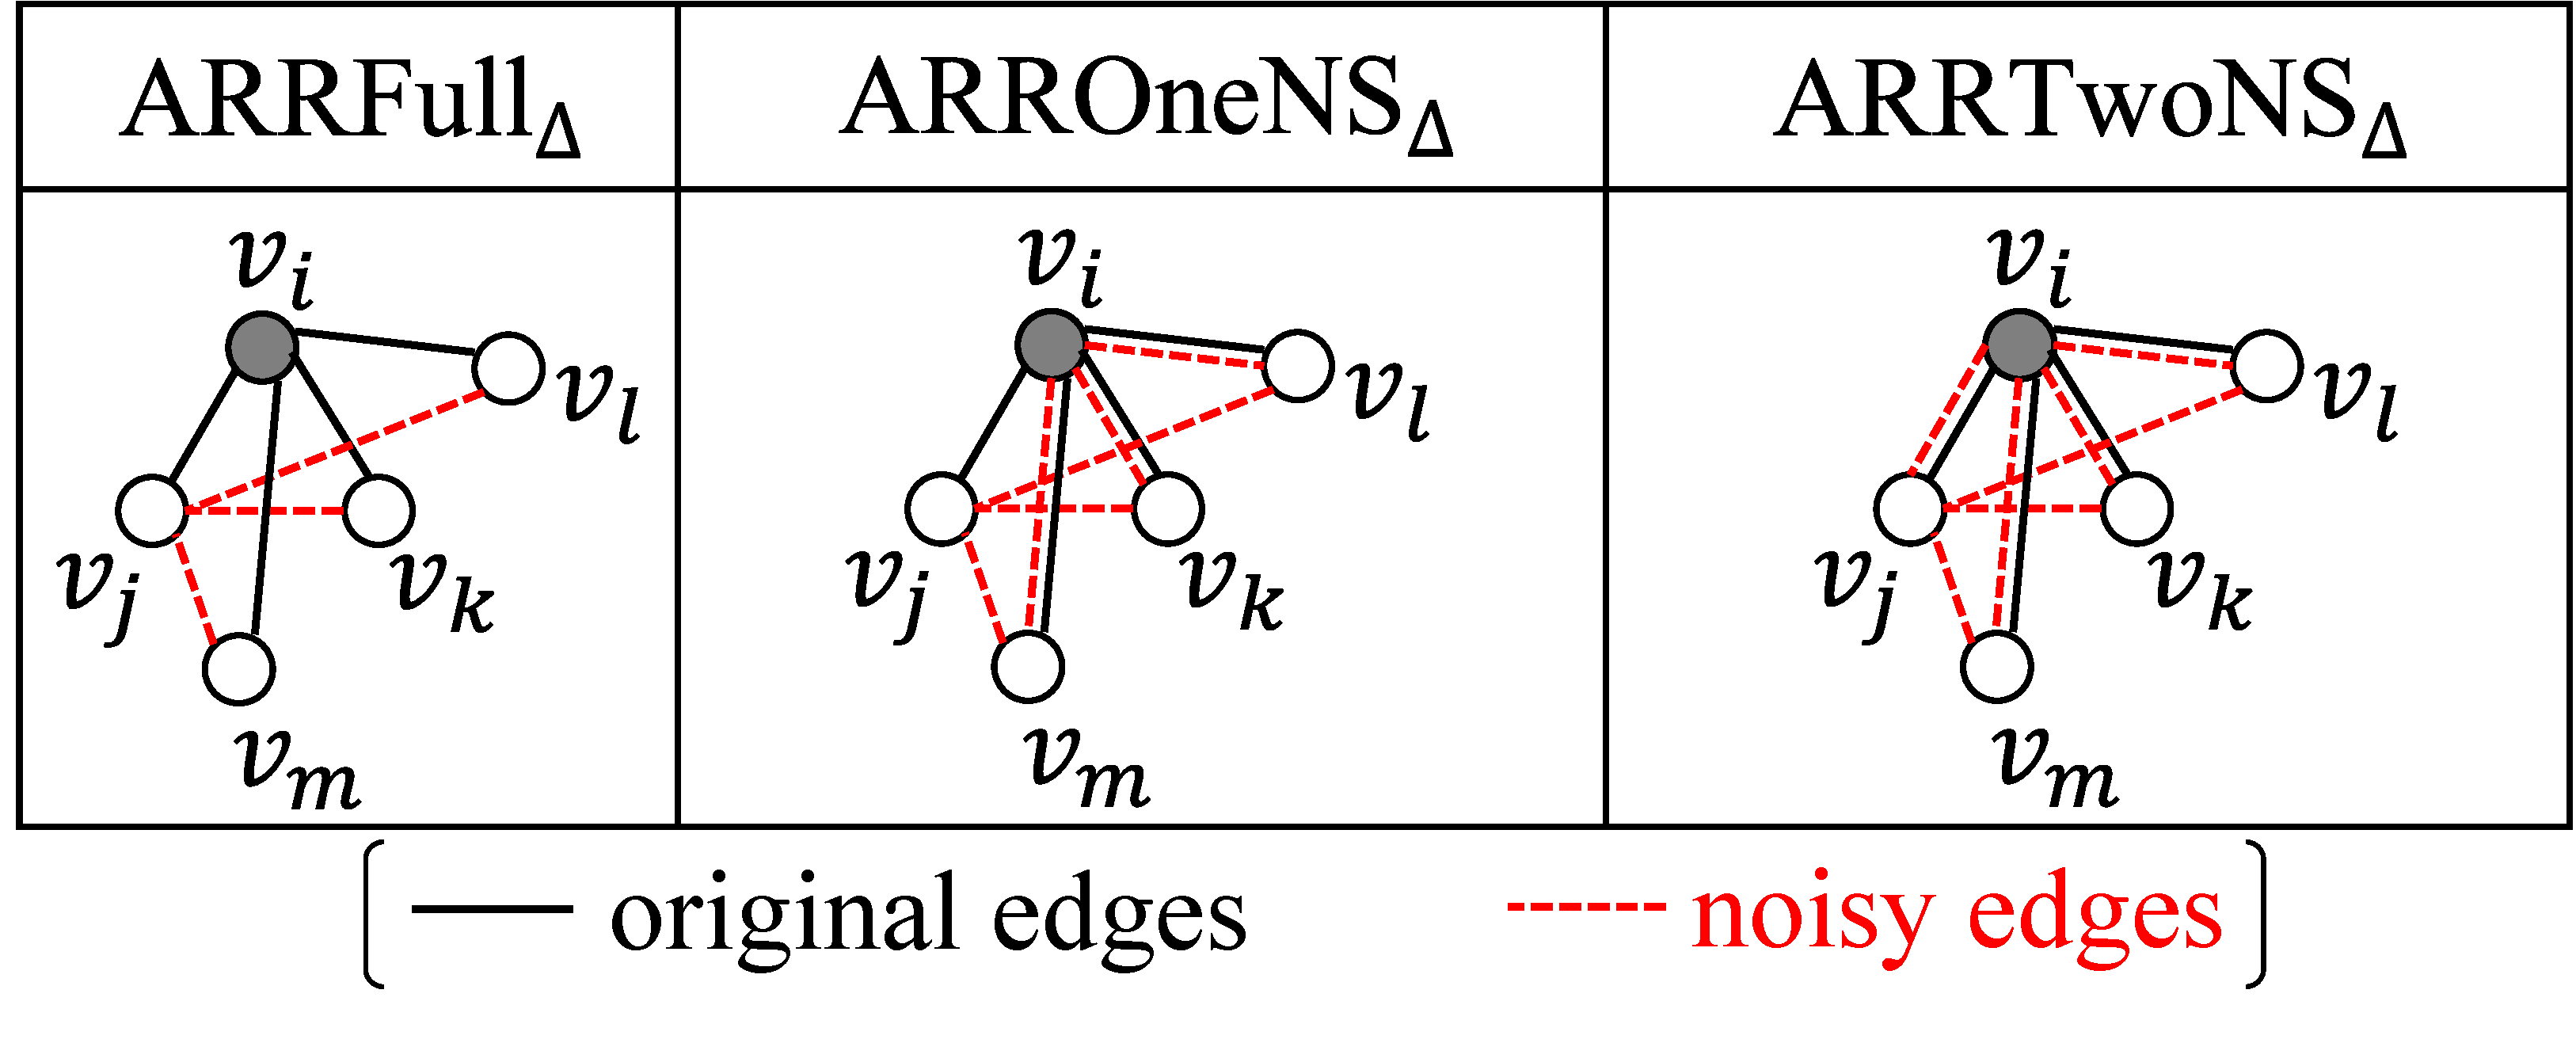
\includegraphics[width=0.78\linewidth]{fig/double_clipping.pdf}
  \vspace{-4mm}
  \caption{Noisy triangles involving edge $(v_i,v_j)$ counted by user $v_i$ ($j<k,l,m<i$).} 
  \label{chap2-fig:reduce_noisy_triangles}
%\end{figure}
\vspace{2mm}
%\begin{figure}[t]
  \centering
  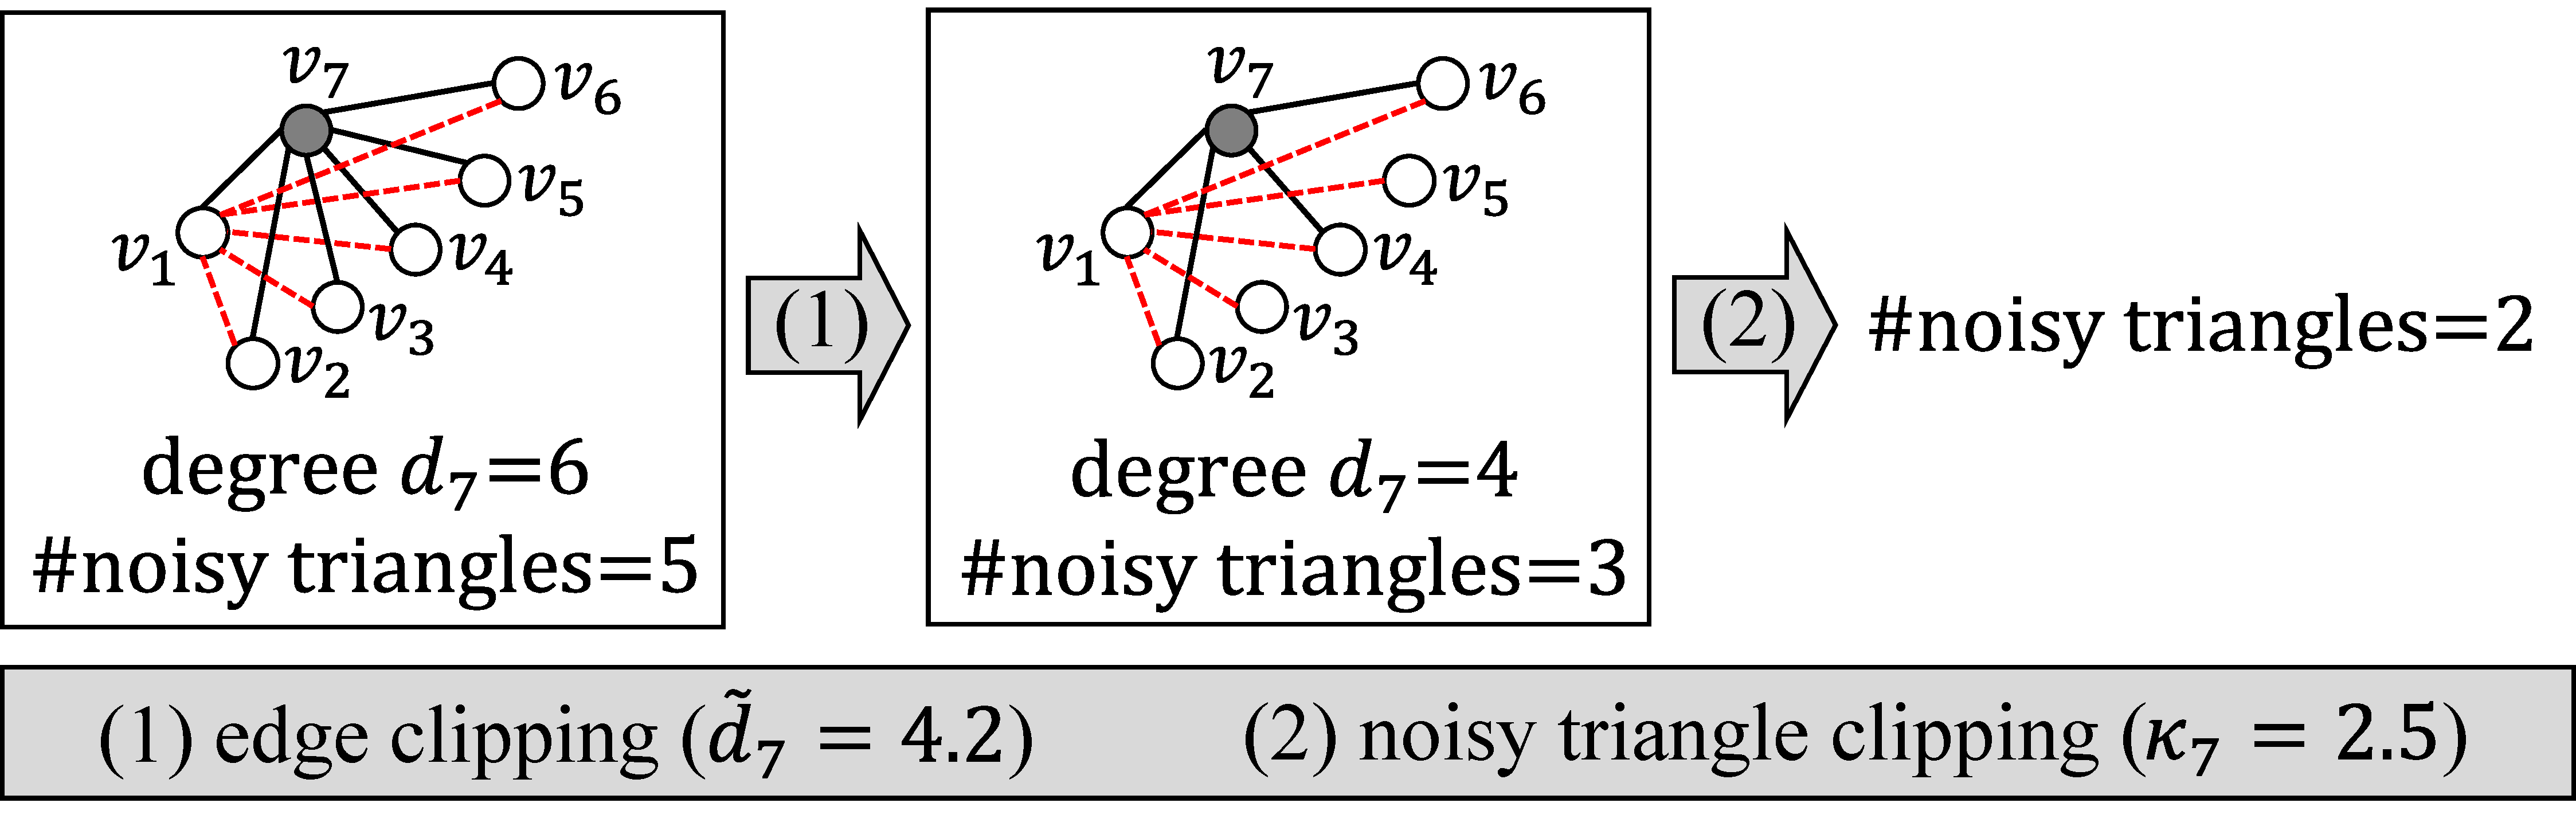
\includegraphics[width=0.99\linewidth]{fig/clip_overview.pdf}
  \vspace{-4mm}
  \caption{Overview of double clipping applied to edge ($v_1,v_7$).} 
  \label{chap2-fig:double-clip_overview}
\end{figure}

% To address the first and second issues explained above, we introduce an edge clipping and triangle clipping, respectively. 
To address these two issues, 
%(i.e., the leakage of $d_i$ and the excess of the noisy triangle count), 
we propose a double clipping technique, which is explained below. 
% which consists of an \textit{adaptive edge clipping} and \textit{noisy triangle clipping}. 

\smallskip
\noindent{\textbf{Algorithm Overview.}}~~Figure~\ref{chap2-fig:double-clip_overview} shows 
% its overview. 
the overview of our double clipping, which consists of an 
% \textit{adaptive edge clipping} 
\textit{edge clipping} 
and \textit{noisy triangle clipping}. 
% The adaptive edge clipping 
The edge clipping 
addresses the first issue (i.e., leakage of $d_i$) 
as follows. 
% by borrowing the idea of adaptive clipping \cite{Andrew_arXiv21,Pichapati_arXiv19} 
% in DP-SGD (Differentially Private Stochastic Gradient Descent). 
% which privately estimates an appropriate clipping threshold in DP-SGD (Stochastic Gradient Descent) \cite{Abadi_CCS16} with DP. 
% Specifically, it 
It privately computes 
a noisy version of 
$d_i$ (denoted by $\td_i$) with edge LDP. 
% Let $\td_i \in \nnreals$ be the private value of $d_i$. 
% user $v_i$ 
% adds the Laplacian noise and some positive constant $\eta \in \nnreals$ to $d_i$ to provide edge LDP 
% and 
Then it 
%performs edge clipping 
%(a.k.a. graph projection \cite{Day_SIGMOD16,Ding_TKDE21,Kasiviswanathan_TCC13,Raskhodnikova_arXiv15}), which 
removes some neighbors from a neighbor list $\bma_i$ so that the degree of $v_i$ never exceeds 
% the private estimate of $d_i$. 
% the private value of $d_i$ 
% (denoted by $\td_i \in \nnreals$). 
% (denoted by $\td_i$). 
the noisy degree $\td_i$. 
This removal process is also known as graph projection \cite{Day_SIGMOD16,Ding_TKDE21,Kasiviswanathan_TCC13,Raskhodnikova_arXiv15}. 
% This kind of technique is called adaptive clipping \cite{Andrew_arXiv21,Pichapati_arXiv19} 
% in DP-SGD (Stochastic Gradient Descent) \cite{Abadi_CCS16} because it privately estimates an appropriate clipping threshold with DP. 
% Adaptive edge clipping 
Edge clipping 
is 
% also 
used in \cite{Imola_USENIX21} to obtain a 
% private value of 
noisy version of 
% the maximum degree 
$d_{max}$. 
%(though ours is to obtain a noisy version of $d_i$). 

% The triangle clipping addresses the second issue (i.e., excess of the noisy triangle count) by reducing the noisy triangle count so that it never exceeds a 
% user-dependent threshold $\kappa_i \in \nnints$. 
The main novelty in our double clipping lies at the \textit{noisy triangle clipping} to address the second issue (i.e., excess of the noisy triangle count). 
% Note that 
This issue appears 
% only 
when 
% each edge is sampled and 
we attempt to reduce the global sensitivity by using 
a very small sampling probability for each edge. 
% value of $\mu$ in the ARR.  
% using a stochastic algorithm such as the ARR. 
Therefore, the noisy triangle clipping has not been studied in the existing works on private triangle counting 
% \cite{Ding_TKDE21,Imola_USENIX21,Karwa_PVLDB11,Kasiviswanathan_TCC13,Song_arXiv18,Sun_CCS19,Ye_ICDE20,Ye_TKDE21,Zhang_SIGMOD15}, 
\cite{Ding_TKDE21,Imola_USENIX21,Karwa_PVLDB11,Kasiviswanathan_TCC13,Sun_CCS19,Ye_ICDE20,Ye_TKDE21,Zhang_SIGMOD15}, 
because they do not apply a sampling technique. 

Our noisy triangle clipping reduces the noisy triangle count so that it never exceeds a 
user-dependent clipping threshold 
$\kappa_i \in \nnreals$. 
% $\kappa_i = \lambda_i \mu^* \td_i$, where $\lambda_i \in \nats$. 
% We call $\kappa_i$ and $\lambda_i$ the \textit{clipping threshold} and \textit{clipping coefficient}, respectively. 
Then a crucial issue is how to set 
an appropriate 
% clipping 
threshold 
$\kappa_i$. 
We theoretically analyze the probability that the noisy triangle count exceeds $\kappa_i$ 
(referred to as the \textit{triangle excess probability}) 
as a function of 
the ARR parameter $\mu$ and the 
% private value $\td_i$ of $d_i$. 
noisy degree $\td_i$. 
% of user $v_i$. 
Then we set $\kappa_i$ so that 
the triangle excess probability 
% the probability 
is very small ($=10^{-6}$ in our experiments). 

We use the clipping threshold $\kappa_i$ as a global sensitivity. 
% of the Laplacian noise. 
Note that $\kappa_i$ provides edge LDP because $\td_i$ provides edge LDP, 
% and $\kappa_i$ depends on only $\mu$ and $\td_i$ 
i.e., immunity to post-processing \cite{DP}. 
$\kappa_i$ is also very small when $\mu \ll 1$, as it is determined based on $\mu$. 

% We also emphasize that our double clipping does \textit{not} assume that $d_{max}$ is public, because it privately computes $\td_i$. 
% by adaptive edge clipping.

\subsection{Algorithms}
\label{chap2-sub:algorithms}
Algorithm~\ref{chap2-alg:clip} shows our double clipping algorithm. 
All the processes are run by user $v_i$ at the second round. 
Thus, there is no interaction with the server in Algorithm~\ref{chap2-alg:clip}.

\setlength{\algomargin}{5mm}
\begin{algorithm}[t]
  \SetAlgoLined
  \KwData{Neighbor list $\bma_i \in \{0,1\}^n$, privacy budget
  $\epsilon_0 \in \nnreals$ 
  $\mu \in [0,\frac{e^{\epsilon_1}}{e^{\epsilon_1} + 1}]$, 
  %$\eta \in \nnreals$.
  $\alpha \in \nnreals$, 
  $\beta \in \nnreals$.
  }
  \KwResult{$\hw_i$.}
  $\mu^* \leftarrow \mu$, $\mu^2$, and $\mu^3$ in F, O, and T, respectively\;
  \tcc{Edge clipping.}
  %$\td_i = \max\{d_i + \Lap(\frac{1}{\epsilon_0}) + \eta$, 0\}\;
  $\td_i = \max\{d_i + \Lap(\frac{1}{\epsilon_0}) + \alpha$, 0\}\;
  \tcc{Remove $d_i - \lfloor \td_i \rfloor$ neighbors if $d_i > \td_i$.}
  $\bma_i \leftarrow \texttt{GraphProjection}(\bma_i, \td_i)$\;
  \tcc{Noisy triangle clipping.}
  \For{$j$ \rm{such that} $a_{i,j} = 1$ \rm{and} $j<i$}{
    $t_{i,j} \leftarrow |\{(v_i,v_j,v_k) : a_{i,k} = 1, (v_j,v_k) \in M_i, j<k<i \}|$\;
  }
%  \tcc{Calculate $\kappa_i$ such that $\kappa_i \in [\mu^* \td_i, \td_i]$.}
   \tcc{Calculate $\kappa_i \in [\mu^* \td_i, \td_i]$ s.t. the triangle excess probability is $\beta$ or less.}
%  \tcc{Calculate $\lambda_i \in \nats$ such that the triangle excess probability is $\beta$ or less.}
  $\kappa_i \leftarrow \texttt{ClippingThreshold}(\mu, \td_i, \beta)$\;
%  $\lambda_i \leftarrow \texttt{ClippingThreshold}(\mu, \td_i, \beta)$\;
%   $\kappa_i \leftarrow \lambda_i \mu^* \td_i$\;
  $t_i \leftarrow \sum_{a_{i,j} = 1, j<i} \min \{t_{i,j}, \kappa_i\}$\;
  $s_i \leftarrow |\{(v_i,v_j,v_k) : a_{i,j} = a_{i,k} = 1, j<k<i\}|$\;
  $w_i \leftarrow t_i - \mu^* \rho s_i$\;
  $\hw_i \leftarrow w_i + \Lap(\frac{\kappa_i}{\epsilon_2})$\;
  \KwRet{$\hw_i$}
  \caption{Our double clipping algorithm. 
  ``F'', ``O'', ``T'' are shorthands for 
  \AlgOne{}, \AlgTwo{}, and \AlgThree{}, respectively.
  All the processes are run by user $v_i$.
  }\label{chap2-alg:clip}
\end{algorithm}

\smallskip
\noindent{\textbf{Edge Clipping.}}~~The edge clipping appears in lines 2-3 of Algorithm~\ref{chap2-alg:clip}. 
It uses a privacy budget $\epsilon_0 \in \nnreals$. 
% for privately computing $d_i$. 

In line 2, user $v_i$ adds the Laplacian noise $\Lap(\frac{1}{\epsilon_0})$ to her degree $d_i$. 
Since adding/removing one edge changes $d_i$ by at most $1$, this process provides $\epsilon_0$-edge LDP. 
$v_i$ also adds some non-negative constant 
% $\eta \in \nnreals$ 
$\alpha \in \nnreals$ 
to $d_i$. 
We add this value so that edge removal (in line 3) occurs with a very small probability; 
e.g., in our experiments, we set $\alpha = 150$, where 
% when $\epsilon_0 = 0.1$ and $\alpha = 150$, 
edge removal occurs with probability $1.5 \times 10^{-7}$ when $\epsilon_0 = 0.1$. 
A similar technique is introduced in \cite{Sun_CCS19} to provide ($\epsilon, \delta)$-DP \cite{DP} with small $\delta$. 
The difference between ours and \cite{Sun_CCS19} is that we perform edge clipping 
% (graph projection) 
to always provide $\epsilon$-DP; i.e., $\delta = 0$.
Let $\td_i \in \nnreals$ be the noisy degree of $v_i$.

In line 3, user $v_i$ calls the function \texttt{GraphProjection}, which performs graph projection as follows; 
if $d_i > \td_i$, randomly remove $d_i - \lfloor \td_i \rfloor$ neighbors from $\bma_i$; otherwise, do nothing. 
Consequently, the degree 
% $d_i$ 
of $v_i$ never exceeds $\td_i$. 

\begin{table*}[t]
  \centering
  \begin{tabular}{|l|c|c|c|}
    \hline
    & \AlgOne & \AlgTwo & \AlgThree \\ \hline
    Privacy 
    & \multicolumn{3}{|c|}{$(\epsilon_0 + \epsilon_1 + \epsilon_2)$-edge LDP and $(\epsilon_0 + \epsilon_1 + \epsilon_2)$-relationship DP} \\ \hline
    %& $\epsilon_0 + \epsilon_1 + \epsilon_2$ & $\epsilon_0 + \epsilon_1 + \epsilon_2$ &
    %$\epsilon_0 + \epsilon_1 + \epsilon_2$ \\ \hline
    Expected $l_2$ loss 
    % & $\frac{2 C_4(G) + S_2(G)}{\mu(1-e^{-\epsilon_1})^2}$ + $\frac{2 \sum_{i=1}^n \kappa_{i}^2}{\mu^2 (1-e^{-\epsilon_1})^2 \epsilon_2^2}$
    % & $O\left(\frac{n d_{max}^3}{\mu(1-e^{-\epsilon_1})^2} + \frac{2 \sum_{i=1}^n \lambda_{i}^2 \td_i^2}{(1-e^{-\epsilon_1})^2 \epsilon_2^2}\right)$
    & $O\left(\frac{n d_{max}^3}{\mu(1-e^{-\epsilon_1})^2} + \frac{2 \sum_{i=1}^n \kappa_{i}^2}{\mu^2(1-e^{-\epsilon_1})^2 \epsilon_2^2}\right)$
    % & $\frac{\mu(12 S_3(G) + 6 P_3(G)) + 6 S_2(G)}{\mu^2(1-e^{-\epsilon_1})^2}$ + $\frac{2 \sum_{i=1}^n \kappa_{i}^2}{\mu^4 (1-e^{-\epsilon_1})^2 \epsilon_2^2}$
    % & $O\left(\frac{n d_{max}^2}{\mu^2(1-e^{-\epsilon_1})^2} + \frac{2 \sum_{i=1}^n \lambda_{i}^2 \td_i^2}{(1-e^{-\epsilon_1})^2 \epsilon_2^2} \right)$
    & $O\left(\frac{n d_{max}^2}{\mu^2(1-e^{-\epsilon_1})^2} + \frac{2 \sum_{i=1}^n \kappa_{i}^2}{\mu^4 (1-e^{-\epsilon_1})^2 \epsilon_2^2} \right)$
    % & $\frac{\mu^2 (12 S_3(G) + 6 P_3(G)) + 6 S_2(G)}{\mu^3(1-e^{-\epsilon_1})^2}$ + $\frac{2 \sum_{i=1}^n \kappa_{i}^2}{\mu^6 (1-e^{-\epsilon_1})^2 \epsilon_2^2}$ \\ \hline
    % & $O\left(\frac{n d_{max}^2}{\mu^3(1-e^{-\epsilon_1})^2} + \frac{2 \sum_{i=1}^n \lambda_{i}^2 \td_i^2}{(1-e^{-\epsilon_1})^2 \epsilon_2^2} \right)$ \\ \hline
    & $O\left(\frac{n d_{max}^2}{\mu^3(1-e^{-\epsilon_1})^2} + \frac{2 \sum_{i=1}^n \kappa_{i}^2}{\mu^6 (1-e^{-\epsilon_1})^2 \epsilon_2^2} \right)$ \\ \hline
    % $l_2$ loss of emp 
    % & $\frac{2 C_4(G) + S_2(G)}{\mu_F(1-e^{-\epsilon_1})^2}$
    % & $\frac{\mu_O(12 S_3(G) + 6 P_3(G)) + 6 S_2}{\mu_O^2(1-e^{-\epsilon_1})^2}$
    % & $\frac{\mu_T^2 (12 S_3(G) + 6 P_3(G)) + 6 S_2}{\mu_T^3(1-e^{-\epsilon_1})^2}$ \\ \hline
    % $l_2$ loss of \Lap{} 
    % & $\frac{2 \sum_{i=1}^n \kappa_{i,F}^2}{\mu_F^2 (1-e^{-\epsilon_1})^2 \epsilon_2^2}$
    % & $\frac{2 \sum_{i=1}^n \kappa_{i,O}^2}{\mu_F^2 (1-e^{-\epsilon_1})^2 \epsilon_2^2}$
    % & $\frac{2 \sum_{i=1}^n \kappa_{i,T}^2}{\mu_F^2 (1-e^{-\epsilon_1})^2 \epsilon_2^2}$ \\ \hline
    $\text{Cost}_{DL}$ & 
    $\mu n^2 \log n$ 
    % $\mu e^{-\epsilon_1} n^2 \log n$ 
    % $\mu_F e^{-\epsilon_1} n(n-1) \log n$ 
    % $(n(n-1) \mu_F \rho + |E| \mu_F (1 - \rho)) \log n$ 
    & 
    $\mu^2 n^2 \log n$ 
    % $\mu^2 e^{-\epsilon_1} n^2 \log n$ 
    % $\mu_O^2 e^{-\epsilon_1} n(n-1) \log n$ 
    & 
    $\mu^3 n^2 \log n$ 
    % $\mu^3 e^{-\epsilon_1} n^2 \log n$ 
    % $\mu_T^3 e^{-\epsilon_1} n(n-1) \log n$ 
    \\ \hline
    $\text{Cost}_{UL}$ & 
    $\mu n \log n$ & $\mu n \log n$ & $\mu n \log n$ 
    % $\mu e^{-\epsilon_1} n \log n$ & $\mu e^{-\epsilon_1} n \log n$ & $\mu e^{-\epsilon_1} n \log n$ 
    \\ \hline
  \end{tabular}
  \vspace{-2mm}
  \caption{Performance guarantees 
  %Privacy, expected $l_2$ loss, and download/upload cost 
  of our three algorithms with double clipping when the edge removal and triangle removal do not occur. 
  %($C_4$: \#$4$-cycles, $P_3$: \#$3$-paths, $S_k$: \#$k$-stars). 
  %($\lambda_i$: clipping coefficient, $\td_i$: noisy degree).
  The expected $l_2$ loss assumes that $\mu$ is small. 
  The download (resp.~upload) cost is an upper-bound in (\ref{chap2-eq:CostDL_F}) 
  %, (\ref{chap2-eq:CostDL_O}), (\ref{chap2-eq:CostDL_T}), 
  (resp.~(\ref{chap2-eq:CostUL_proposal})).
  %approximation when $d_{max} \ll n$. 
  %the graph $G$ is sparse.
  }
  \label{chap2-tab:privacy_utility_cost}
\end{table*}

\smallskip
\noindent{\textbf{Noisy Triangle Clipping.}}~~The noisy triangle clipping appears in lines 4-11 of Algorithm~\ref{chap2-alg:clip}. 

% First, 
In lines 4-6, 
user $v_i$ calculates the number $t_{i,j} \in \nnints$ of noisy triangles ($v_i, v_j, v_k$) ($j<k<i$) involving $(v_i,v_j)$ 
(as shown in Figure~\ref{chap2-fig:reduce_noisy_triangles}). 
%such that only one edge ($v_j, v_k$) is noisy 
% for her neighbor $v_j$. 
% (lines 4-6). 
Note that the total number $t_i$ of noisy triangles of $v_i$ can be expressed as: 
$t_i = \sum_{a_{i,j}=1, j<i} t_{i,j}$. 
In line 7, $v_i$ calls the function \texttt{ClippingThreshold}, which calculates a clipping threshold 
% $\kappa_i$ 
$\kappa_i \in [\mu^* \td_i, \td_i]$ 
($\mu^* = \mu$, $\mu^2$, and $\mu^3$ in 
``F'', ``O'', and ``T'', respectively) 
based on the ARR parameter $\mu$ and the noisy degree $\td_i$ so that 
% $\kappa_i \in [\mu^* \td_i, \td_i]$ 
% ($\mu^* = \mu$, $\mu^2$, and $\mu^3$ in 
% ``F'', ``O'', and ``T'', respectively) 
% and 
the triangle excess probability does not exceed some constant $\beta \in \nnreals$. 
% $\kappa_i$ takes a value between $\mu^* \td_i$ and $\td_i$; i.e., $\kappa_i \in [\mu^* \td_i, \td_i]$. 
We explain how to calculate 
% $\kappa_i$ from $\mu$ and $\td_i$ 
the triangle excess probability 
in Section~\ref{chap2-sub:clip_theoretical_analysis}. 
% in detail. 
In line 8, $v_i$ calculates the total number $t_i$ of noisy triangles by summing up $t_{i,j}$, with the exception that $v_i$ adds $\kappa_i$ 
%(rather than $t_{i,j}$) 
if $t_{i,j} > \kappa_i$. 
%$t_{i,j}$ exceeds $\kappa_i$. 
In other words, triangle removal occurs 
% when 
if 
$t_{i,j} > \kappa_i$. 
% Consequently, 
Then, 
the number 
% $t_{i,j}$ 
of noisy triangles involving $(v_i,v_j)$ never exceeds $\kappa_i$. 

Lines 9-11 in Algorithm~\ref{chap2-alg:clip} are the same as lines 12-14 in Algorithm~\ref{chap2-alg:unify}, except that 
the global sensitivity in the former (resp.~latter) is $\kappa_i$ (resp.~$d_{max}$). 
% the global sensitivity in Algorithm~\ref{chap2-alg:clip} is $\kappa_i$. 
Line 11 in Algorithm~\ref{chap2-alg:clip} provides $\epsilon_2$-edge LDP because the number of triangles involving $(v_i,v_j)$ is now upper-bounded by $\kappa_i$. 

\smallskip
\noindent{\textbf{Our Entire Algorithms with Double Clipping.}}~~We can run our algorithms \AlgOne{}, \AlgTwo{}, \AlgThree{} with double clipping just by replacing lines 11-14 in Algorithm~\ref{chap2-alg:unify} with lines 2-11 in Algorithm~\ref{chap2-alg:clip}. 
That is, after calculating $\hw_i$ by Algorithm~\ref{chap2-alg:clip}, $v_i$ uploads $\hw_i$ to the server. 
Then the server calculates an estimate of $f_\triangle(G)$ as $\hf_\triangle(G) = \frac{1}{\mu^*(1-\rho)}\sum_{i=1}^n \hw_i$. 
%as in line 17 of Algorithm~\ref{chap2-alg:unify}. 
% where $\mu^* = \mu$, $\mu^2$, and $\mu^3$ in 
% ``F'', ``O'', and ``T'', respectively). 

We also note that the input $d_{max}$ in Algorithm~\ref{chap2-alg:unify} is no longer necessary thanks to the edge clipping; i.e., our entire algorithms with double clipping do not assume that $d_{max}$ is public. 
% , because $v_i$ privately calculates $d_i$ by edge clipping.

\subsection{Theoretical Analysis}
\label{chap2-sub:clip_theoretical_analysis}
% \paragraph{Privacy}
% \smallskip
We now perform a theoretical analysis on the privacy and utility of our double clipping. 
% All the proofs appear in \arxiv{Appendix~\ref{chap2-sec:proof_double_clip}}\conference{the full version \cite{Imola_arXiv22}}. 

\smallskip
\noindent{\textbf{Privacy.}}~~We begin with the privacy guarantees:
% Our algorithms with double clipping have the following privacy guarantees:
\begin{theorem}\label{chap2-thm:privacy_DC}
  For $i \in [n]$, 
  let $\calR_i^1, \calR_i^2(M_i)$ be the randomizers used by user $v_i$ in
  rounds $1$ and $2$ of our algorithms with double clipping (Algorithms~\ref{chap2-alg:unify} and \ref{chap2-alg:clip}). 
  Let $\calR_i(\bma_i) = (\calR_i^1(\bma_i), \calR_i^2(M_i)(\bma_i))$ 
  be the composition of the two randomizers. 
  Then,
  $\calR_i$ satisfies $(\epsilon_0 + \epsilon_1 + \epsilon_2)$-edge LDP, 
  %for $i \in [n]$, 
  and $(\calR_1,
  \ldots, \calR_n)$ satisfies $(\epsilon_0 + \epsilon_1 + \epsilon_2)$-relationship DP.
\end{theorem}

\smallskip
\noindent{\textbf{Utility.}}~~Next, we show the triangle excess probability: 
% the probability that the noisy triangle count $t_{i,j}$ exceeds $\kappa_i$:

\begin{theorem}\label{chap2-thm:triangle_excess}
%Let $\mu^* = \mu_F$ and $\mu_O^2$ in \AlgOne{} and \AlgTwo{}, respectively. 
%In \AlgOne{} and \AlgTwo{}, 
%In \AlgOne{}, \AlgTwo{}, \AlgThree{}, 
% Let $\mu_F, \mu_O, \mu_T \in [0,\frac{e^{\epsilon}}{e^{\epsilon_1} + 1}]$. 
% For $i \in [n]$, let $\td_i \in \nnreals$ be a noisy degree of user $v_i$ output by edge clipping. 
% Let $\kappa_i$
In Algorithm~\ref{chap2-alg:clip}, the triangle excess probability (i.e., probability that the number of noisy triangles $t_{i,j}$ involving edge $(v_i, v_j)$ exceeds a clipping threshold $\kappa_i$) is:
  \begin{align}
    \hspace{-1mm} \Pr(t_{i,j} > \kappa_i) &\leq \textstyle{\exp \left[-\td_i D \left(\frac{\kappa_i}{\td_i} \parallel \mu \right) \right]} \label{chap2-eq:AlgI_clip_bound} \\
    \hspace{-1mm} \Pr(t_{i,j} > \kappa_i) &\leq \textstyle{\exp \left[-\td_i D \left(\frac{\kappa_i}{\td_i} \parallel \mu^2 \right) \right]} \label{chap2-eq:AlgII_clip_bound}\\
%   \end{align}
%   \begin{align}
    \hspace{-1mm} \Pr(t_{i,j} > \kappa_i) &\leq 
    \textstyle{\mu \exp \left[-\td_i D \left(\frac{\max\{\kappa_i,\mu^2 \td_i\}}{\td_i} \parallel \mu^2 \right) \right]}
    % \begin{cases}
    %     \mu_T \exp \left[-\td_i D \left(\frac{\kappa_i}{\td_i} \parallel \mu_T^2 \right) \right]   &   \mathrm{(if}~ \kappa_i \geq \mu_T^2 \td_i)\\
    %     \mu_T   &   \mathrm{(if}~ \mu_T^3 \td_i \leq \kappa_i < \mu_T^2 \td_i),
    % \end{cases}
    \label{chap2-eq:AlgIII_clip_bound}
  \end{align}
  in \AlgOne{}, \AlgTwo{}, and \AlgThree{}, respectively, 
  where 
  % $\mu^* = \mu_F$ and $\mu_O^2$ in \AlgOne{} and \AlgTwo{}, respectively, and 
  $D(p_1 \parallel p_2)$ is the Kullback-Leibler divergence between two Bernoulli distributions; i.e., 
  %$D(p_1 \parallel p_2) = p_1 \log \frac{p_1}{p_2} + (1-p_1) \log \frac{1-p_1}{1-p_2}$.
  %with $p_1$ and $p_2$:
  %the Bernoulli($p_1$) and Bernoulli($p_2$) distribution; 
\begin{align*}
    \textstyle{D(p_1 \parallel p_2) = p_1 \log \frac{p_1}{p_2} + (1-p_1) \log \frac{1-p_1}{1-p_2}.}
\end{align*}
\end{theorem}
In all of (\ref{chap2-eq:AlgI_clip_bound}), (\ref{chap2-eq:AlgII_clip_bound}), and (\ref{chap2-eq:AlgIII_clip_bound}), we use the Chernoff bound, which is known to be reasonably tight \cite{Arratia_BMB89}. 

\smallskip
\noindent{\textbf{Setting $\kappa_i$.}}~~The function \texttt{ClippingThreshold} in Algorithm~\ref{chap2-alg:clip} sets a clipping threshold $\kappa_i$ of user $v_i$ based on Theorem~\ref{chap2-thm:triangle_excess}. 
Specifically, we set $\kappa_i = \lambda_i \mu^* \td_i$, where $\lambda_i \in \nats$, and calculate $\lambda_i$ as follows. 
We initially set $\lambda_i = 1$ and keep increasing $\lambda_i$ by $1$ 
% initially set $\kappa_i = \mu^* \td_i$ and keep increasing $\kappa_i$ by $\mu^* \td_i$ 
until the upper-bound (i.e., right-hand side of (\ref{chap2-eq:AlgI_clip_bound}), (\ref{chap2-eq:AlgII_clip_bound}), or (\ref{chap2-eq:AlgIII_clip_bound})) is smaller than or equal to the triangle excess probability $\beta$. 
In our experiments, we set $\beta = 10^{-6}$. 
% We call $\lambda_i$ the \textit{clipping coefficient} of $v_i$. 

\smallskip
\noindent{\textbf{Large $\kappa_i$ of \AlgThree{}.}}~~By 
% In our experiments, we set $\mu$ so that $\mu$ in \AlgOne{} is equal to $\mu^2$ in \AlgTwo{} and also equal to $\mu^3$ in \AlgThree{}. 
% Then by 
(\ref{chap2-eq:AlgI_clip_bound}) and (\ref{chap2-eq:AlgII_clip_bound}), the upper-bound on the triangle excess probability is the same between \AlgOne{} and \AlgTwo{}. 
% However, 
In contrast, 
\AlgThree{} has a larger upper-bound. 
For example, 
when $\kappa_i = 15 \mu^* \td_i$, $\mu^* = 10^{-3}$, and $\td_i=1000$, 
the right-hand sides of (\ref{chap2-eq:AlgI_clip_bound}), (\ref{chap2-eq:AlgII_clip_bound}), and (\ref{chap2-eq:AlgIII_clip_bound}) are $2.5 \times 10^{-12}$, $2.5 \times 10^{-12}$, and $3.3 \times 10^{-2}$, respectively. 
Consequently, \AlgThree{} has a larger global sensitivity $\kappa_i$ for the same value of $\beta$.

% \smallskip
% \noindent{\textbf{\AlgTwo{} vs. \AlgThree{}.}}~~Now we explain the reason that \AlgTwo can reduce the global sensitivity more effectively than \AlgThree (as described in Section~\ref{chap2-sub:algorithms_overview}).  
% using Figure~\ref{chap2-fig:reduce_noisy_triangles}. 
% As with \AlgOne, 
We can explain a large global sensitivity $\kappa_i$ of \AlgThree{} as follows. 
The number $t_{i,j}$ of noisy triangles involving $(v_i,v_j)$ in 
\AlgOne{} is expected to be around $\mu d_i$ because one noisy edge is in each noisy triangle (as in Figure~\ref{chap2-fig:reduce_noisy_triangles}) and all noisy edges are independent. 
For the same reason, $t_{i,j}$ in \AlgTwo{} is expected to be around $\mu^2 d_i$.  
% \AlgTwo{} is expected to be around $\mu_O^2 d_i$ because two noisy edges are in each noisy triangle (as in Figure~\ref{chap2-fig:reduce_noisy_triangles}) and all noisy edges are independent. 
% 
However, 
% the number of noisy triangles involving $(v_i,v_j)$ 
$t_{i,j}$ in \AlgThree{} is \textit{not} expected to be around $\mu^3 d_i$, because all the noisy triangles have noisy edge $(v_i,v_j)$ in common (as in Figure~\ref{chap2-fig:reduce_noisy_triangles}). 
Then, 
% the expected noisy triangle count 
the expectation of $t_{i,j}$ 
largely depends on the presence/absence of the noisy edge $(v_i,v_j)$; i.e., if noisy edge $(v_i,v_j)$ exists, 
it is $\mu^2 d_i$; otherwise, $0$. 
% Consequently, 
% the noisy triangle count (i.e., global sensitivity) 
% the global sensitivity 
Thus, 
$\kappa_i$ 
cannot be effectively reduced by double clipping. 
% Section~\ref{chap2-sub:clip_theoretical_analysis} shows a more formal result on this. 

\smallskip
\noindent{\textbf{Summary.}}~~The 
% privacy, expected $l_2$ loss, download/upload cost 
performance guarantees 
of our three algorithms with double clipping can be summarized in Table~\ref{chap2-tab:privacy_utility_cost}.

% The expected $l_2$ loss can be expressed $O(n d_{max}^3)$, $O(n d_{max}^2)$, and $O(n d_{max}^2)$, 
% For the $l_2$ loss, 
The first and second terms of the expected 
$l_2$ loss are the $l_2$ loss of empirical estimation and that of the Laplacian noise, respectively. 
For small 
% $\mu_F$ ($=\mu_O^2 = \mu_T^3$), 
$\mu$, 
the $l_2$ loss of empirical estimation can be expressed as $O(n d_{max}^3)$, $O(n d_{max}^2)$, and $O(n d_{max}^2)$ in \AlgOne{}, \AlgTwo{}, \AlgThree{}, respectively, as explained in Section~\ref{chap2-sub:algorithms_theoretical_analysis}. 
% (when we regard $\epsilon_1$ and $\epsilon_2$ as constants). 
% The large $l_2$ loss of \AlgOne{} is caused by the number $C_4$ of $4$-cycles that is written as $O(n d_{max}^3)$. 
The $l_2$ loss of the Laplacian noise is 
$O(\sum_{i=1}^n \kappa_i^2)$, 
% $O(\sum_{i=1}^n \lambda_i^2 \td_i^2)$, 
which is much smaller than $O(n d_{max}^2)$. 
% when $\lambda_i$ is small. 
Thus, our \AlgTwo{} that effectively reduces $\kappa_i$ provides the smallest error, 
% for a large graph or dense graph where $C_4$ is large, 
as shown in our experiments.

We also note that 
both the space and the time complexity to compute and send $M_i$ in our algorithms 
% time and space complexity of 
% our algorithms at the server side 
are $O(\mu^* n^2)$ (as $|E'| =  O(\mu^* n^2)$), which is much smaller than \cite{Imola_USENIX21} ($=O(n^2)$). 


\section{Experiments}
\label{chap2-sec:experiments}

% Based on the theoretical results in Sections~\ref{chap2-sub:algorithms_theoretical_analysis} and \ref{chap2-sub:clip_theoretical_analysis}, we would like to pose the following questions:
To evaluate each component of our algorithms in Sections~\ref{chap2-sec:algorithms} and \ref{chap2-sec:double_clip} as well as our entire algorithms (i.e., \AlgOne, \AlgTwo, \AlgThree with double clipping), we pose the following three research questions:
%\begin{enumerate}
\begin{description}[leftmargin=9.75mm]
% \begin{itemize}[leftmargin=9.7mm]
    \item[RQ1.] 
    %\item 
    How do our three triangle counting algorithms 
    (i.e., \AlgOne, \AlgTwo, \AlgThree) in Section~\ref{chap2-sec:algorithms} compare with each other in terms of accuracy?
    \item[RQ2.] 
    %\item 
    How much does our double clipping technique in Section~\ref{chap2-sec:double_clip} decrease the estimation error?
    %increases the utility?
    \item[RQ3.] 
    %\item 
    How much do our entire algorithms reduce the communication cost, compared to the existing algorithm~\cite{Imola_USENIX21}, while keeping high utility (e.g., relative error $\ll 1$)?
% \end{enumerate}
\end{description}
% \end{itemize}
% To answer to the questions, we designed our experiments.
% We explain our experimental setup in Section~\ref{chap2-sub:setup}. 
% Note that we compare our entire algorithms with the two-rounds algorithm~\cite{Imola_USENIX21} 
% because one-round algorithms result in a very large estimation error, as shown in Appendix~\ref{chap2-sec:one-round}. 
% See Appendix~\ref{chap2-sec:one-round} for the comparison with one-round algorithms.
In Appendix~\ref{chap2-sec:one-round}, we also compare our entire algorithms with one-round algorithms.


% focus on the two-rounds algorithms in our experiments. 
% Below we explain our experimental set-up (Section~\ref{chap2-sub:setup}) and report results (Section~\ref{chap2-sub:results}) to answer to the three questions.

\subsection{Experimental Set-up}
\label{chap2-sub:setup}
In our experiments, we used two real graph datasets:

\smallskip
\noindent{\textbf{Gplus.}}~~The Google+ dataset~\cite{McAuley_NIPS12} (denoted by \GPlus{}) 
% includes a social graph collected from users who had shared circles. 
was collected from users who had shared circles. 
% includes publicly available network information collected from users who had shared circles. 
% ego-networks that represent Google+ users who had shared circles and whose network information is publicly available. 
From the dataset, we 
% extracted 
constructed 
a social graph $G=(V,E)$ with $107614$ nodes (users) and $12238285$ edges, where 
% an edge represents that a user follows or is followed by another one. 
edge $(v_i,v_j) \in E$ represents that $v_i$ follows or is followed by $v_j$. 
The average (resp.~maximum) degree in $G$ is $113.7$ (resp.~$20127$). 

\smallskip
\noindent{\textbf{IMDB.}}~~The IMDB (Internet Movie Database)~\cite{IMDB_GD05} (denoted by \IMDB{}) includes a bipartite graph between $896308$ actors and $428440$ movies. 
From this, we constructed a graph $G=(V,E)$ with $896308$ nodes (actors) and $57064358$ edges, where edge $(v_i,v_j) \in E$ represents that $v_i$ and $v_j$ have played in the same movie. 
The average (resp.~maximum) degree in $G$ is $63.7$ (resp.~$15451$). 
Thus, \IMDB{} is more sparse than \GPlus{}. 

\smallskip
In \conference{the full version \cite{Imola_arXiv22}}\arxiv{Appendix~\ref{chap2-sec:BAmodel}}, we also evaluate our algorithms using a synthetic graph based on the Barab\'{a}si-Albert model~\cite{NetworkScience}, which has a power-law degree distribution. 
%We report the results in 
%\conference{the full version \cite{Imola_arXiv22}}\arxiv{Appendix~\ref{chap2-sec:BAmodel}}.

% In our three triangle counting algorithms, we set 
% the ARR parameter $\mu$ so that $\mu$ in \AlgOne{} is equal to $\mu^2$ in \AlgTwo{} and also equal to $\mu^3$ in \AlgThree{}; i.e., $\CostDL{}$ is the same between the three algorithms. 
% Let $\mu^* = \mu$, $\mu^2$, and $\mu^3$ in \AlgOne{}, \AlgTwo{}, and \AlgThree{}, respectively. 
We evaluated our algorithms while changing $\mu^*$, where $\mu^* = \mu$, $\mu^2$, and $\mu^3$ in \AlgOne{}, \AlgTwo{}, and \AlgThree{}, respectively. 
$\CostDL{}$ is the same between the three algorithms. 
We typically 
set the total privacy budget $\epsilon$ to $\epsilon=1$ 
% or $2$ 
(at most $2$) 
because it is acceptable in many practical scenarios \cite{DP_Li}. 

In our double clipping, we set $\alpha = 150$ and $\beta = 10^{-6}$ so that both edge removal and triangle removal occur with a very small probability ($\leq 10^{-6}$ when $\epsilon_0 = 0.1$). 
% \commentT{Will write how to set $\td_i$ and $\kappa_i$ in double clipping.}
Then for each algorithm, we evaluated the relative error between the true triangle count $f_\triangle(G)$ and its estimate $\hf_\triangle(G)$. 
% (as described in Section~\ref{chap2-sub:LDP}). 
Since the estimate $\hf_\triangle(G)$ varies depending on the randomness of LDP mechanisms, we ran each algorithm $\tau \in \nats$ times ($\tau=20$ and $10$ for \GPlus{} and \IMDB{}, respectively) and averaged the relative error over the $\tau$ cases.

\subsection{Experimental Results}
\label{chap2-sub:results}

\smallskip
% \noindent{\textbf{Three Algorithms w/ Lap.}}~~
\noindent{\textbf{Performance Comparison.}}~~First, 
we 
% evaluated our algorithms with the Laplacian noise at the second round. 
evaluated our algorithms with the Laplacian noise. 
% and compared them with the existing two-rounds algorithm in \cite{Imola_USENIX21}. 
Specifically, we evaluated all possible combinations of our three algorithms with and without our double clipping (six combinations in total) and compared them with 
the existing two-rounds algorithm in~\cite{Imola_USENIX21}.  
% the algorithm in~\cite{Imola_USENIX21}.  
For algorithms with double clipping, we divided the total privacy budget $\epsilon$ as: 
% used $\frac{\epsilon}{10}$ for the adaptive edge clipping, and the remaining budget 
% $\epsilon_0: \epsilon_1: \epsilon_2 = 0.1: 0.45: 0.45$.
$\epsilon_0 = \frac{\epsilon}{10}$ and 
$\epsilon_1 = \epsilon_2 = \frac{9\epsilon}{20}$. 
Here, we set a very small budget ($\epsilon_0 = \frac{\epsilon}{10}$) for edge clipping because the degree has a small sensitivity (sensitivity$=1$). 
For algorithms without double clipping, we divided $\epsilon$ as $\epsilon_1 = \epsilon_2 = \frac{\epsilon}{2}$ and 
used the maximum degree $d_{max}$ as the global sensitivity. 
% We emphasize again that our algorithms with double clipping do not assume that $d_{max}$ is public.

\begin{figure}[t]
  \centering
  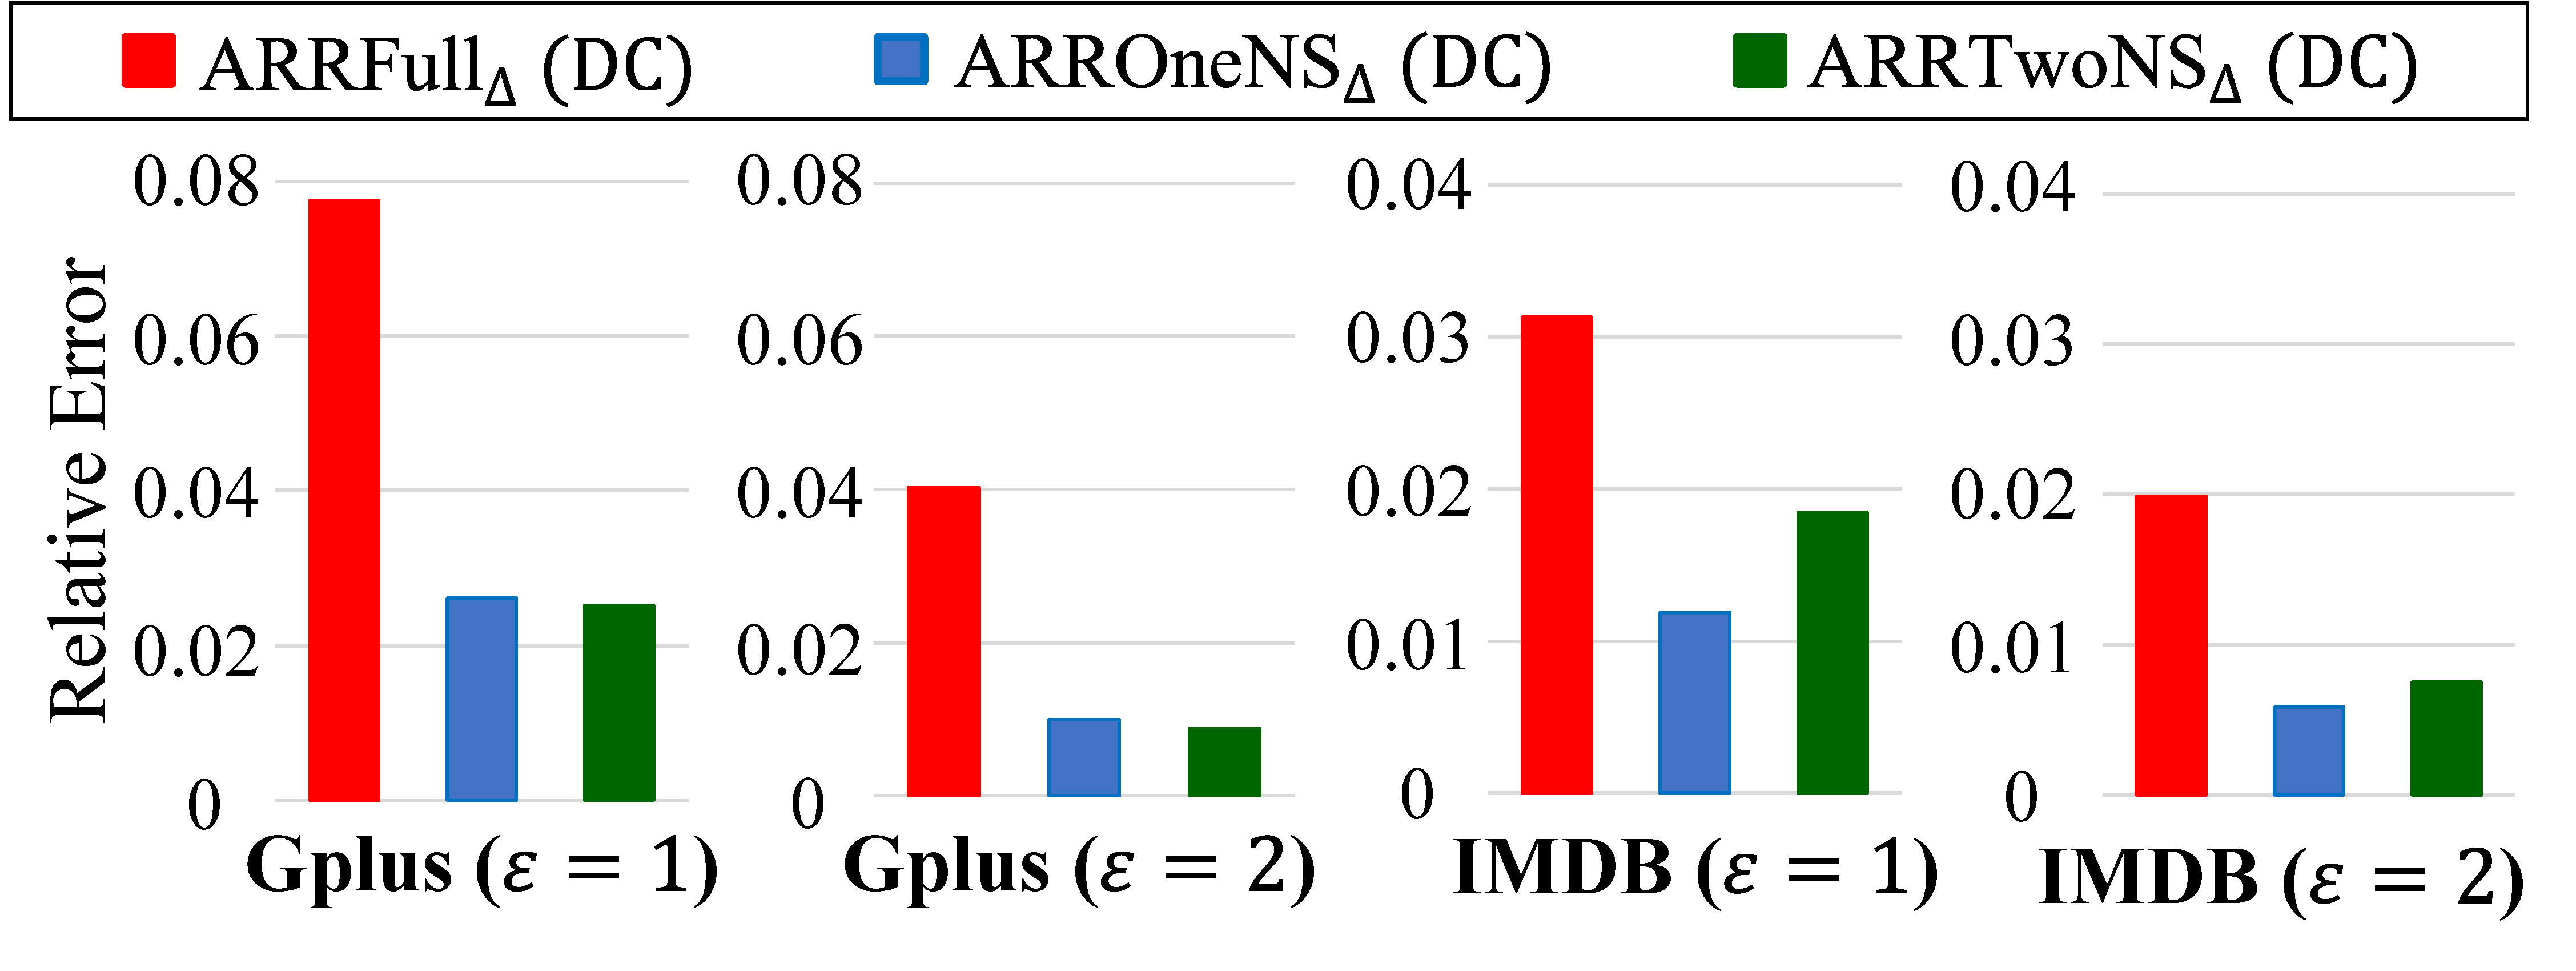
\includegraphics[width=0.96\linewidth]{fig/res2_w_Lap_abst2.pdf}
  \vspace{-6mm}
  \caption{Relative error of our three algorithms with double clipping (``DC'') when $\epsilon=1$ or $2$ and %$\mu_F=10^{-3}$ 
  $\mu^*=10^{-3}$ 
  ($n=107614$ in \GPlus{}, $n=896308$ in \IMDB{}).} 
  \label{chap2-fig:res2_w_Lap_abst}
%\end{figure}
 \vspace{1mm}
%\begin{figure}[t]
  \centering
  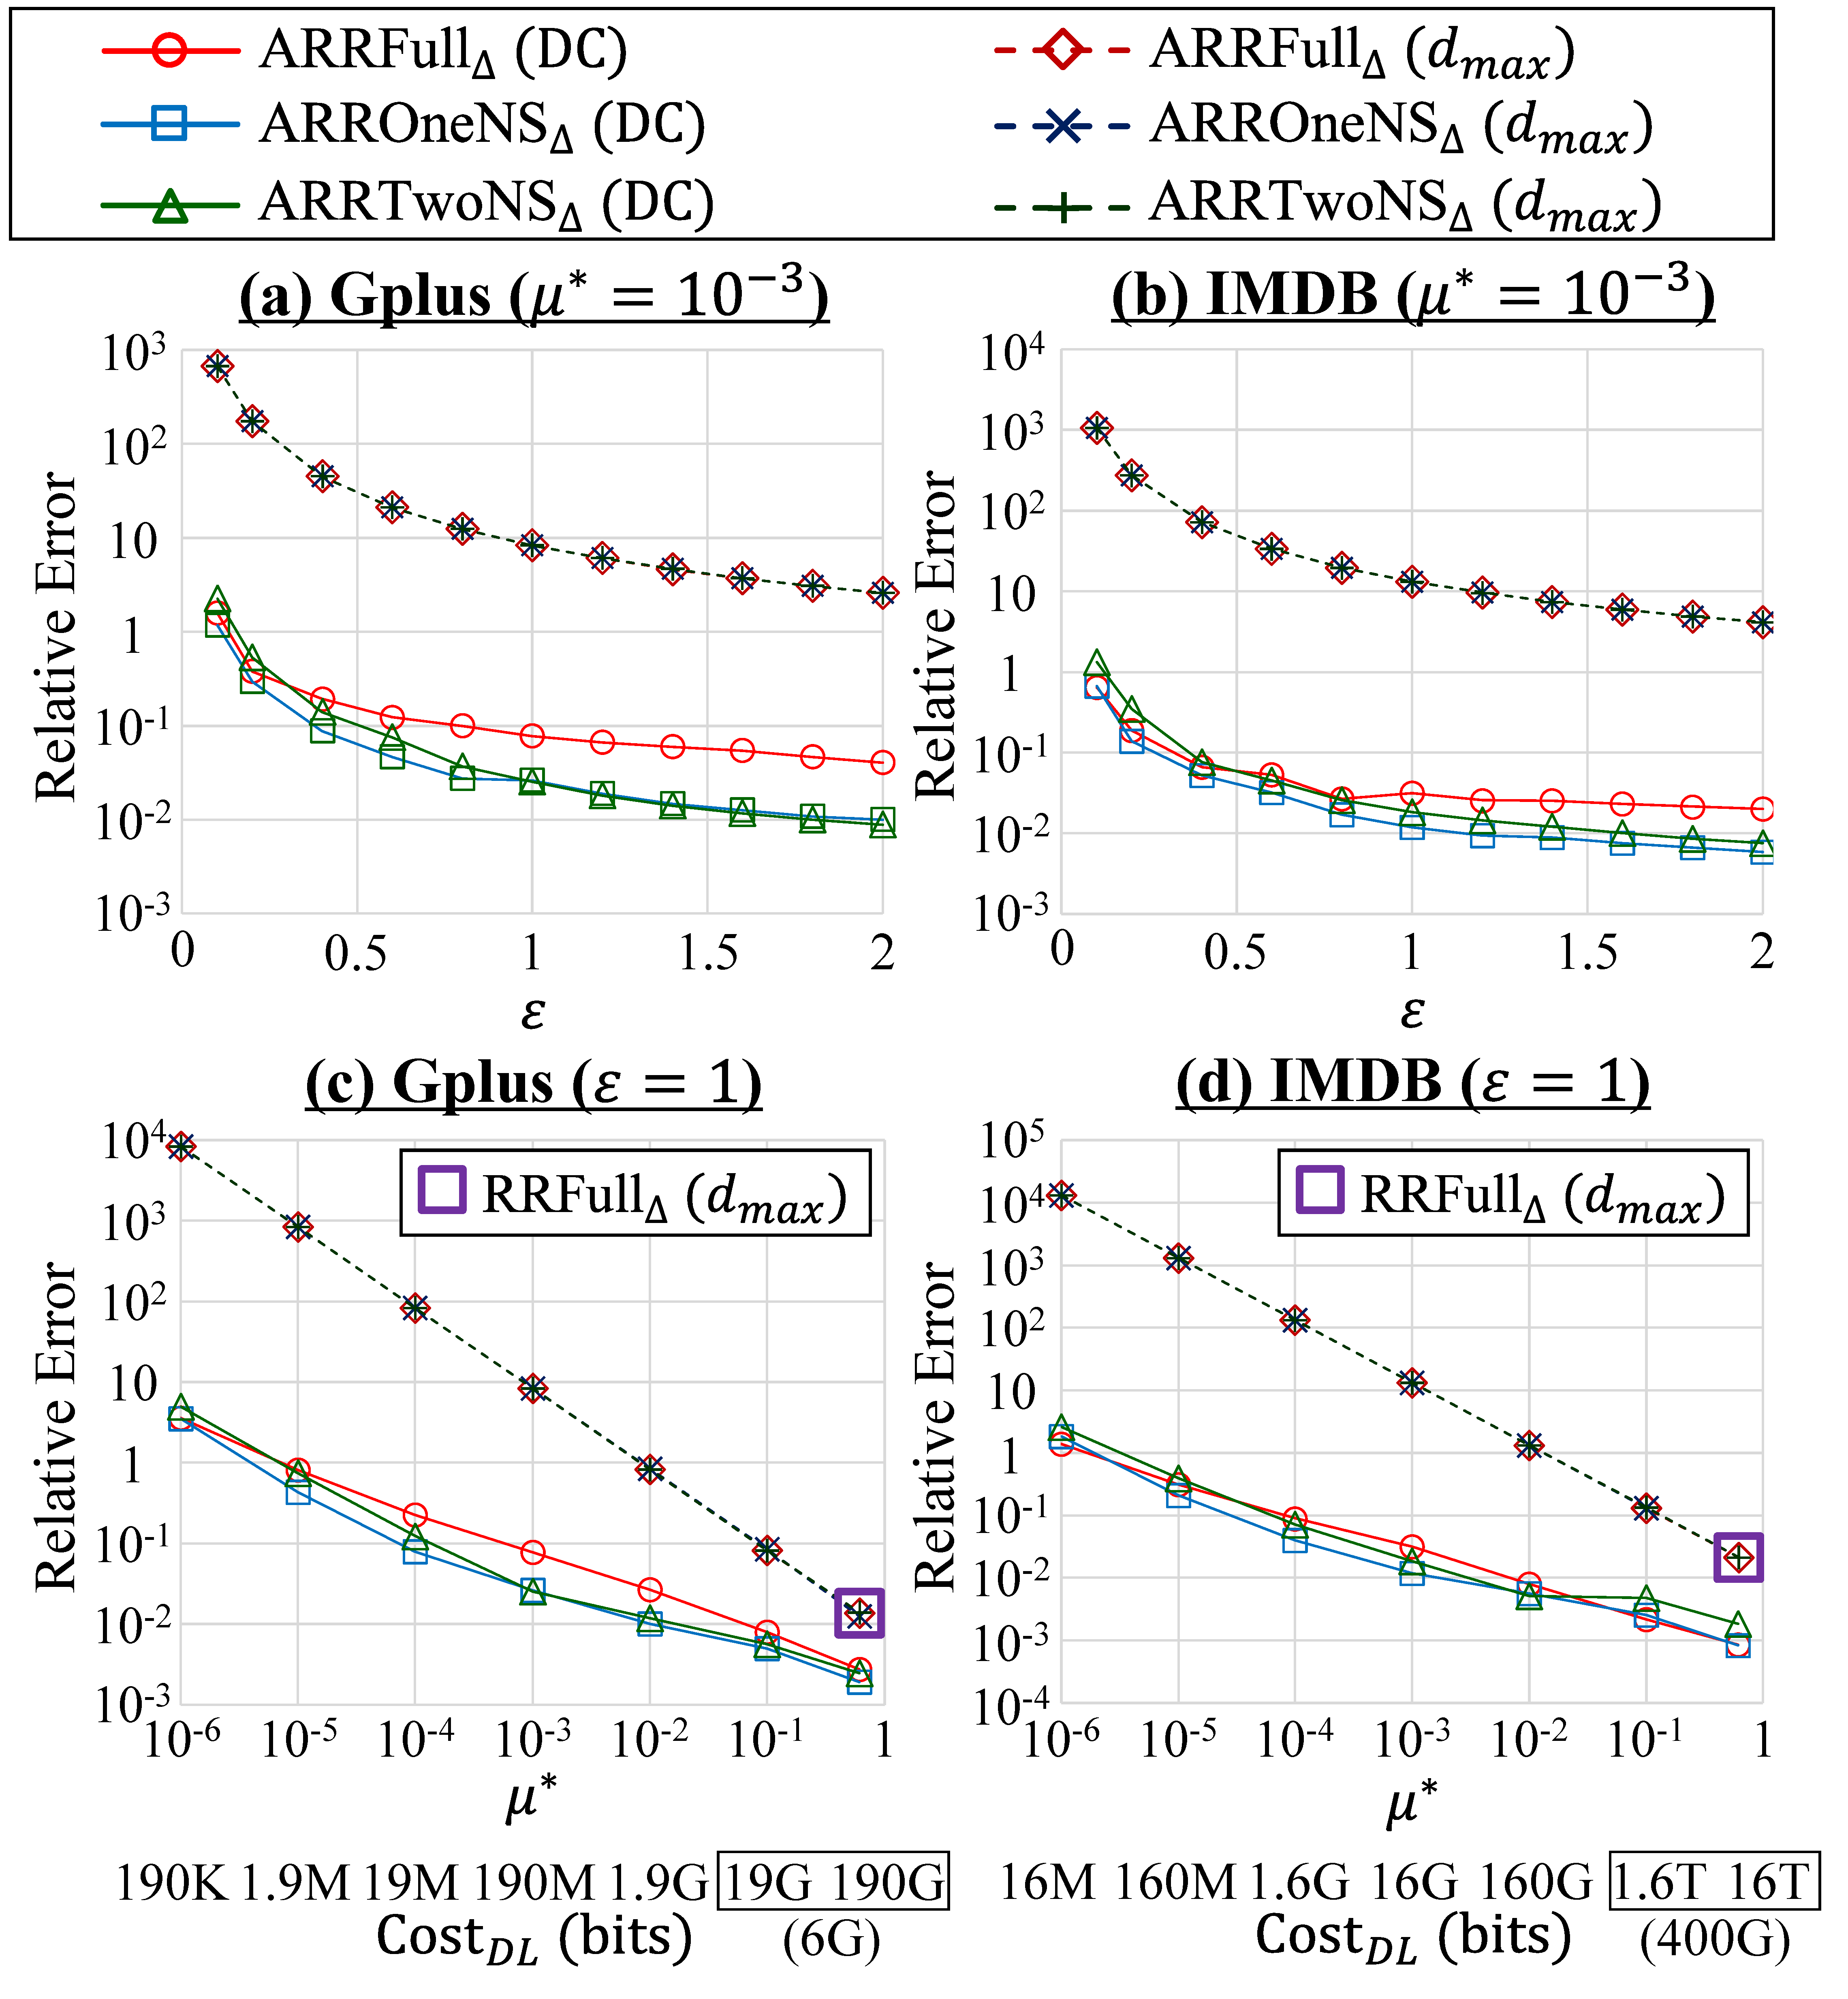
\includegraphics[width=0.99\linewidth]{fig/res2_w_Lap.pdf}
  \vspace{-5mm}
  \caption{Relative error of our three algorithms with (``DC'') or without (``$d_{max}$'') double clipping ($n=107614$ in \GPlus{}, $n=896308$ in \IMDB{}). \AlgSec{} is the 
  %two-rounds 
  algorithm in~\cite{Imola_USENIX21}. 
  $\CostDL$ is 
  %calculated by 
  an upper-bound in 
  (\ref{chap2-eq:CostDL_F}). 
  %Note that 
  When $\mu^* \geq 0.1$, 
  %(marked with squares), 
  $\CostDL$ can be $6$ Gbits and $400$ Gbits in \GPlus{} and \IMDB{}, respectively, by downloading only 0/1 for each pair of users $(v_j,v_k)$.} 
  \label{chap2-fig:res2_w_Lap}
\end{figure}

% \begin{table}[t]
% \caption{Basic notations.} 
% \centering
% \hbox to\hsize{\hfil
% \begin{tabular}{l|l|l}
% \hline
% Algorithm		&	\GPlus{} ($\epsilon=1$) &  \IMDB{}  ($\epsilon=1$)\\
% \hline
% \AlgOne{}   &   $0.078$   &   $0.031$\\
% \hline
% \end{tabular}
% \hfil}
% \label{chap2-tab:res2_w_Lap_abst}
% \end{table}

Figures~\ref{chap2-fig:res2_w_Lap_abst} and \ref{chap2-fig:res2_w_Lap} show the results. 
Figure~\ref{chap2-fig:res2_w_Lap_abst} highlights the relative error of our three algorithms with double clipping when $\epsilon=1$ or $2$ and $\mu^*=10^{-3}$. 
% Figure \ref{chap2-fig:res2_w_Lap} shows the results. 
``DC'' (resp.~``$d_{max}$'') represents algorithms with (resp.~without) double clipping. 
\AlgSec{} (marked with purple square) in Figure~\ref{chap2-fig:res2_w_Lap} (c) and (d) represents the two-rounds algorithm in~\cite{Imola_USENIX21}. 
Note that this is a special case of our \AlgOne{} without sampling ($\mu =\frac{e^{\epsilon_1}}{e^{\epsilon_1}+1} = 0.62$). 
% as described in Section~\ref{chap2-sub:algorithms_overview}. 
Figure~\ref{chap2-fig:res2_w_Lap} (c) and (d) also show the download cost $\CostDL$ calculated by 
(\ref{chap2-eq:CostDL_F}). 
Note that 
when $\mu^* \geq 0.1$ (marked with squares), 
$\CostDL$ can be $6$Gbits and $400$Gbits in \GPlus{} and \IMDB{}, respectively, by downloading only 0/1 for each pair of users $(v_j,v_k)$; $\CostDL = \frac{(n-1)(n-2)}{2}$ in this case. 
% $\CostDL$ is $400$Gbits and $6$Gbits in \GPlus{} and \IMDB{}, respectively, when user $v_i$ downloads only 0/1 for each 
% pair of users $(v_j,v_k)$ ($\CostDL = \frac{(n-1)(n-2)}{2}$ in this case). 

Figures~\ref{chap2-fig:res2_w_Lap_abst} and \ref{chap2-fig:res2_w_Lap} show that our \AlgTwo{} (DC) 
% with double clipping 
provides the best (or almost the best) performance in all cases. 
This is because \AlgTwo{} (DC) introduces the $4$-cycle trick 
% (shown in Figure~\ref{chap2-fig:four-cycle}) 
and effectively reduces the global sensitivity of the Laplacian noise by double clipping. 
% \AlgThree{} (DC) is outperformed by \AlgTwo{} (DC), 
% \AlgTwo{} (DC) outperforms \AlgThree{} (DC), 
% especially when $\epsilon$ or $\mu_F$ ($=\mu_O^2 = \mu_T^3$) is small 
% (e.g., $\epsilon=0.1$ to $0.8$, $\mu_F=10^{-6}$ to $10^{-4}$). 
% There are two reasons for this: 
% (1) \AlgThree{} cannot effectively reduce the global sensitivity by double clipping,
% (2) the Laplacian noise increases with decrease in $\epsilon$ or $\mu_F$, 
% This is because \AlgThree{} cannot effectively reduce the global sensitivity by double clipping and the Laplacian noise increases with decrease in $\epsilon$ or $\mu_F$ 
% and has a non-negligible effect on the estimation error for small $\epsilon$ or $\mu_F$, 
% (as shown in Table~\ref{chap2-tab:privacy_utility_cost} of Section~\ref{chap2-sub:clip_theoretical_analysis}). 
% The difference between \AlgTwo{} (DC) and \AlgOne{} (DC) is also small for very small $\epsilon$ or $\mu_F$ (e.g., $\epsilon=0.1$, $\mu_F=10^{-6}$) because the Laplacian noise is dominant in this case. 
% Later, we will also 
% provide a detailed investigation of the relation between the Laplacian noise and the relative error while changing $n$. 
% to answer our research question RQ1. 
Later, we will 
% also 
% provide a detailed investigation of 
investigate 
the effectiveness of the $4$-cycle trick in detail 
by not adding the Laplacian noise. 
% and 
We will also investigate 
%the relation between the Laplacian noise and the relative error 
the impact of the Laplacian noise 
while changing $n$. 

Figure~\ref{chap2-fig:res2_w_Lap} also shows that 
the relative error is almost the same between our three algorithms without double clipping (``$d_{max}$'') and that it is too large. 
% the relative error of our three algorithms without double clipping is too large and that it is almost the same between the three. 
This is because $\Lap(\frac{d_{max}}{\epsilon_2}$) is too large and dominant. 
The relative error is significantly reduced by introducing our double clipping in all cases. 
% For example, our \AlgTwo{} (DC) without sampling ($\mu_F =\frac{e^{\epsilon_1}}{e^{\epsilon_1}+1}$)
For example, when $\mu^* = 10^{-3}$, our double clipping reduces the relative error of \AlgTwo{} by two or three orders of magnitude. 
% \AlgTwo{} (DC) also reduces the expected download size by $\mu_F = \mu_O^2 = 10^{-3}$ while keeping roughly the same relative error as the algorithm in~\cite{Imola_USENIX21}, thanks to double clipping. 
The improvement is larger for smaller $\mu^*$. 

In \conference{the full version \cite{Imola_arXiv22}}\arxiv{Appendix~\ref{chap2-sec:EC_DC}}, we also evaluate the effect of edge clipping and noisy triangle clipping independently and show that each component significantly reduces the relative error. 

\smallskip
\noindent{\textbf{Communication Cost.}}~~From Figure~\ref{chap2-fig:res2_w_Lap} (c) and (d), we can explain how much our algorithms can reduce the download cost while keeping high utility, e.g., relative error $\ll 1$. 

For example, when we use the algorithm in \cite{Imola_USENIX21}, the download cost is 
$\CostDL = 400$ Gbits in \IMDB{}. 
% $\CostDL = 400$ Gbits and $6$ Gbits in \GPlus{} and \IMDB{}, respectively. 
Thus, when the download speed is $20$ Mbps 
% (which is a 
(recommended speed in YouTube \cite{YouTube_speed}), every user $v_i$ needs 6 hours to download the message $M_i$, which is far from practical. 
In contrast, our \AlgTwo{} (DC) can reduce it to 
% $100$ 
$160$ 
Mbits (8 seconds when $20$ Mbps download rate) or less 
while keeping relative error $= 0.21$, 
% (relative error $= 0.21$), 
% or $1$ Gbits (relative error $= 0.040$). 
% Consequently, every user needs only 
% 5 
% 8 
% or 50 
% seconds or less, 
which is practical and a dramatic improvement over \cite{Imola_USENIX21}. 
% Therefore, private triangle counting is now practical.

We also note that since $d_{max} \ll n$ in \IMDB{}, 
% the ARR outputs ``1'' with probability $\mu e^{-\epsilon_1}$ in most cases
% the download cost 
$\CostDL$ of our \AlgTwo{} (DC) 
can also be roughly approximated by $60$ Mbits (3 seconds) by replacing $\mu$ with $\mu e^{-\epsilon_1}$ in 
(\ref{chap2-eq:CostDL_F}). 
%(\ref{chap2-eq:CostDL_O}). 

% We also note that the upload cost is much smaller; e.g., by (\ref{chap2-eq:CostUL_proposal}), $\CostUL{} = 11$ Mbits in \IMDB{} even when $\mu=1$. 
% Thus, it is not an issue.

\smallskip
% \noindent{\textbf{Three Algorithms w/o Lap.}}~~
\noindent{\textbf{4-Cycle Trick.}}~~We 
% first evaluated 
also investigated 
% how well our two algorithms \AlgTwo{} and \AlgThree{} address the $4$-cycle issue of \AlgOne{} 
the effectiveness of our $4$-cycle trick in \AlgTwo{} and \AlgThree{} 
% (shown in Figure~\ref{chap2-fig:four-cycle}) 
in detail. 
% explained in Section~\ref{chap2-sub:algorithms_overview}. 
% the relation between the $4$-cycle issue 
To this end, we evaluated our three algorithms when we did \textit{not} add the Laplacian noise at the second round. 
% (i.e., $\epsilon_2 = \infty$). 
Note that they do not provide edge LDP, as $\epsilon_2 = \infty$. 
The purpose here is to purely investigate the effectiveness of the $4$-cycle trick 
% issue 
related to our first research question RQ1. 
% We will report experimental results of the three algorithms with the Laplacian noise later. 

\begin{figure}[t]
  \centering
  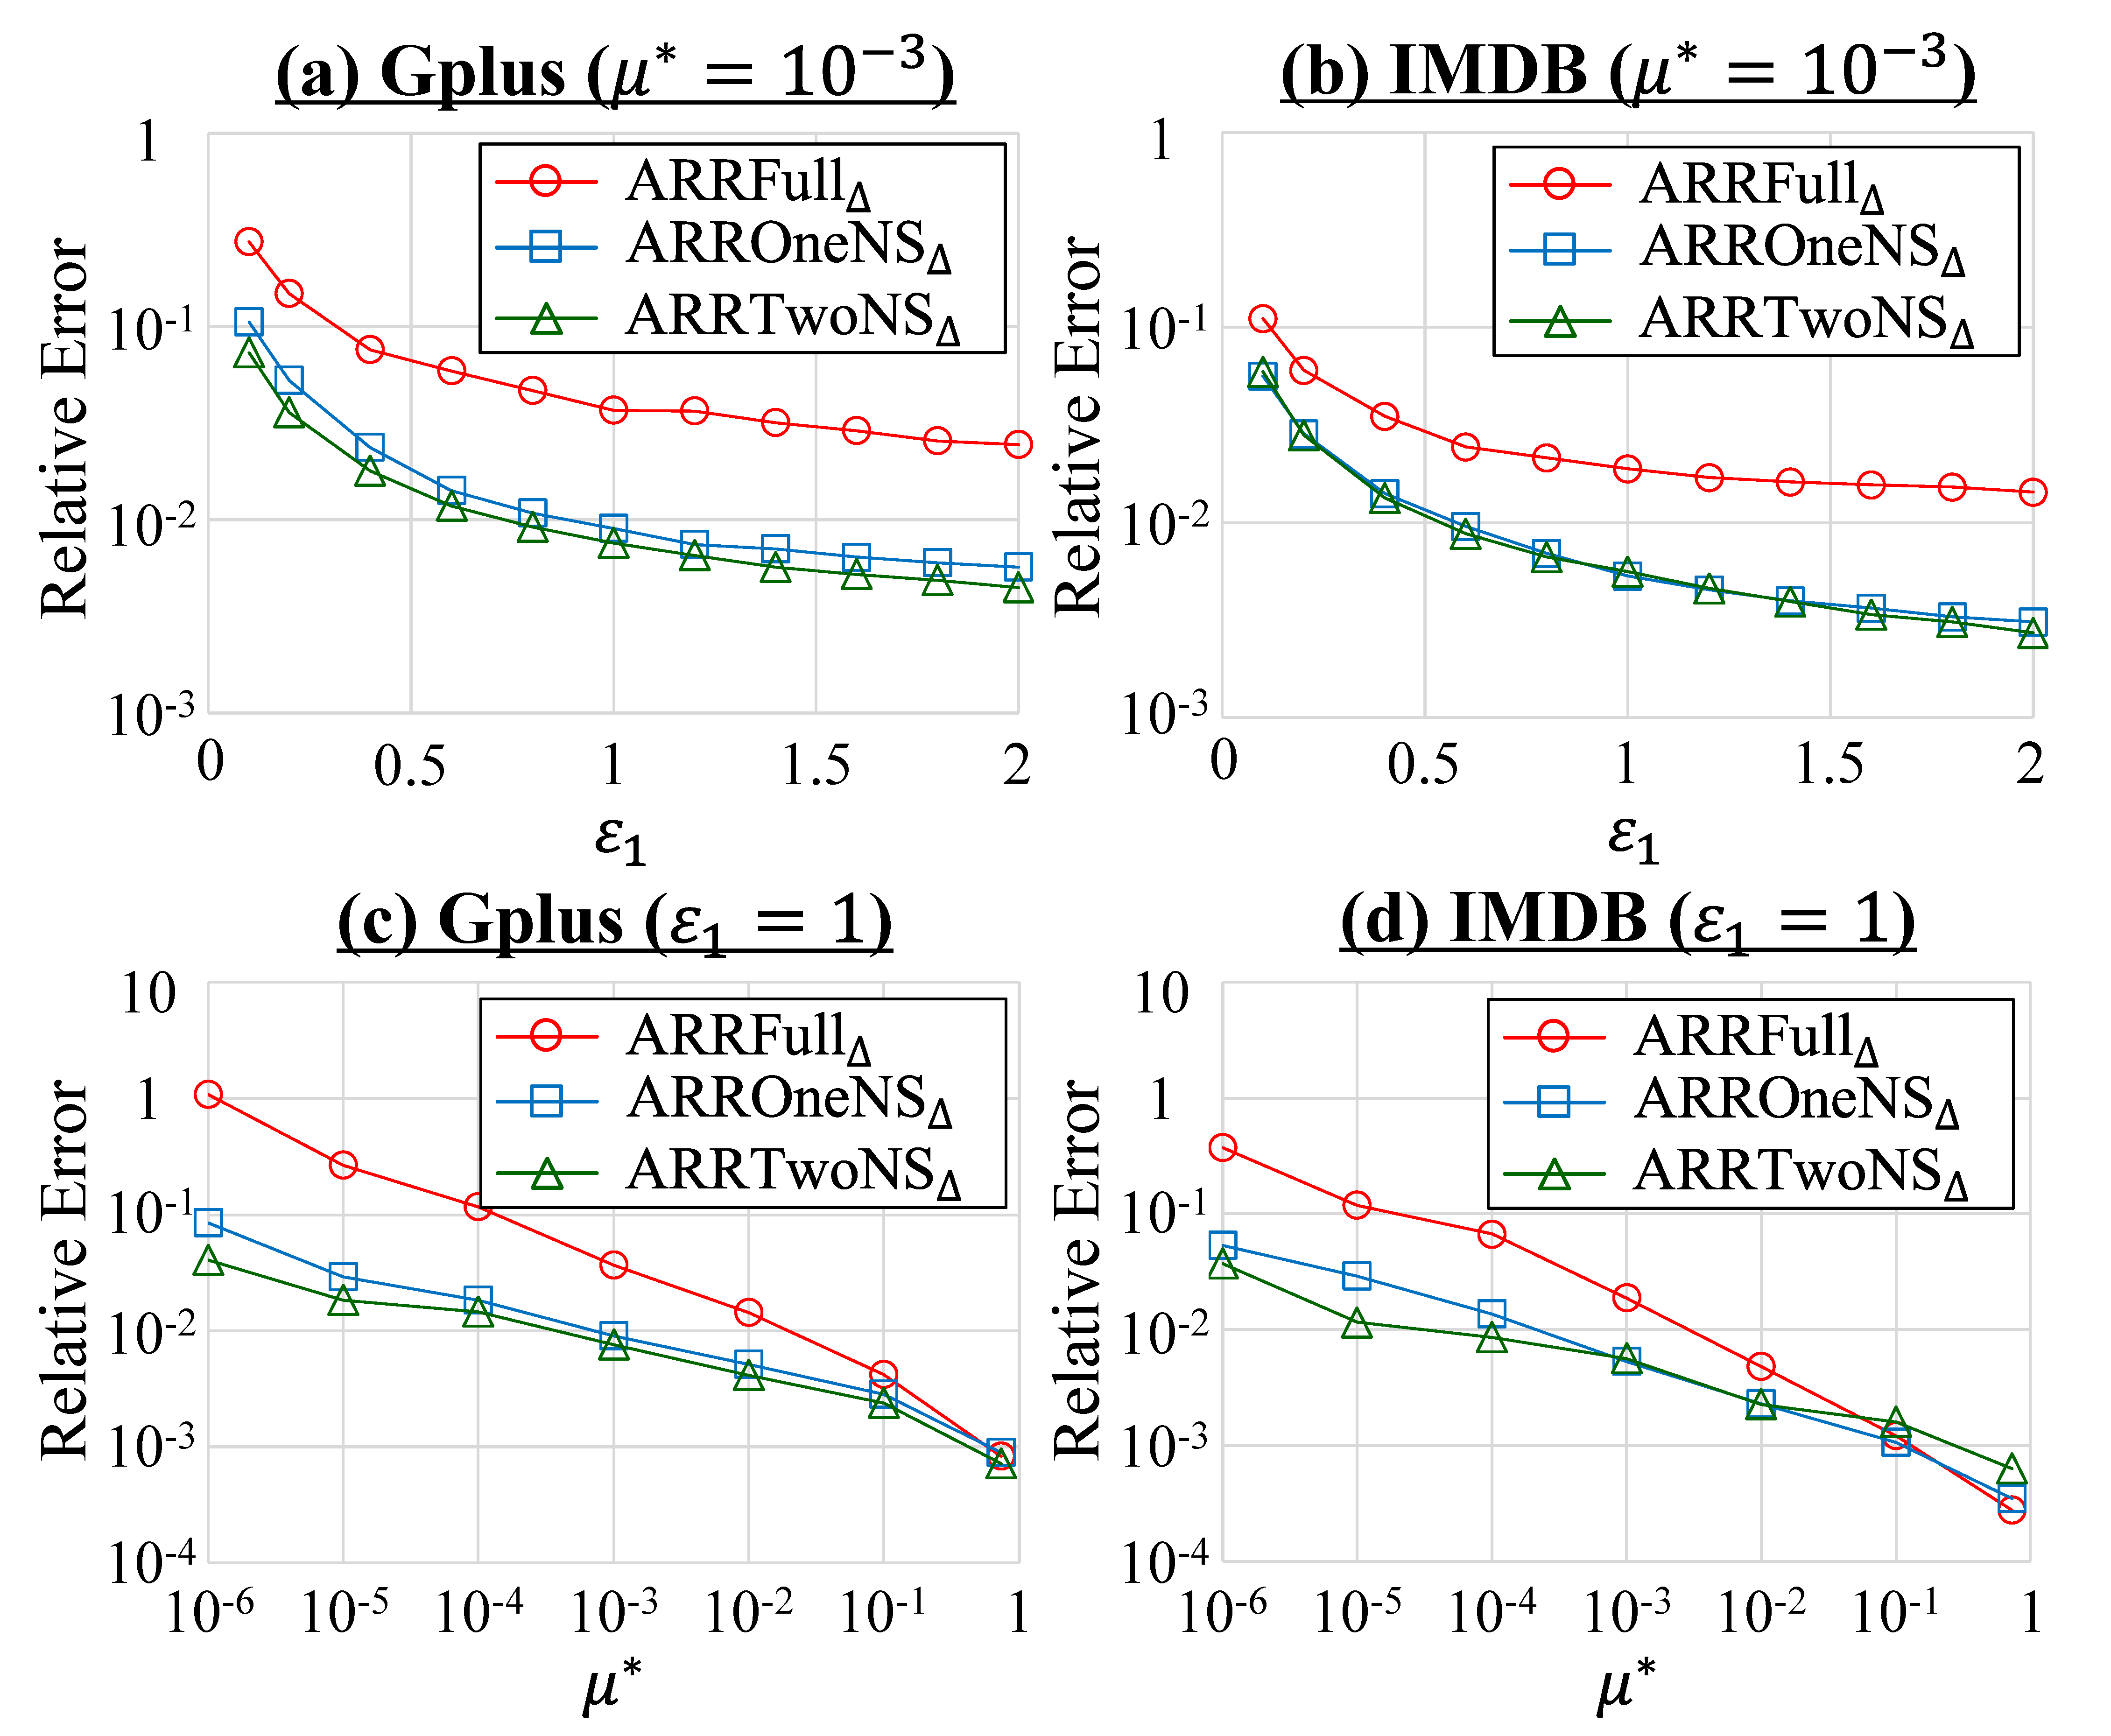
\includegraphics[width=0.99\linewidth]{fig/res1_wo_Lap.pdf}
  \vspace{-5mm}
  \caption{Relative error of our three algorithms without the Laplacian noise 
  % at the second round 
  ($n=107614$ in \GPlus{}, $n=896308$ in \IMDB{}).} 
  \label{chap2-fig:res1_wo_Lap}
\end{figure}

% We first evaluated our three triangle counting algorithms with double clipping. 
Figure~\ref{chap2-fig:res1_wo_Lap} shows the results, where 
% $\mu_F$ (resp.~$\epsilon_1$) is changed from $10^{-6}$ to $1$ (resp.~$0.1$ to $2$). 
% $\epsilon_1$ (resp.~$\mu_F$) is changed from $0.1$ to $2$ (resp.~$10^{-6}$ to $\frac{e^{\mu_F}}{e^{\mu_F} + 1}$). 
$\epsilon_1$ and 
% $\mu_F$ ($= \mu_O^2 = \mu_T^3$) 
$\mu^*$ 
are changed to various values. 
Figure~\ref{chap2-fig:res1_wo_Lap} shows that \AlgTwo{} and \AlgThree{} significantly outperform \AlgOne{} when 
% $\mu_F$ 
$\mu^*$ 
is small. 
This is because in both \AlgTwo{} and \AlgThree{}, 
% the first term in the expected $l_2$ loss 
the factors of 
% $S_3$ (\#3-stars) and $P_3$ (\#3-paths) 
$C_4$ (\#4-cycles) and $S_3$ (\#3-stars) 
in the expected $l_2$ loss 
diminish 
for small $\mu$, 
% as 
% $\mu_F$ ($= \mu_O^2 = \mu_T^3$) 
% the parameter $\mu$ in the ARR 
% goes to $0$, 
as explained in Section~\ref{chap2-sub:algorithms_theoretical_analysis}. 
In other words, \AlgTwo{} and \AlgThree{} effectively address the $4$-cycle issue. 
Figure~\ref{chap2-fig:res1_wo_Lap} also shows that \AlgThree{} slightly outperforms \AlgTwo{} when $\mu^*$ is small. 
% (e.g., $10^{-6}$ to $10^{-4}$). 
This is because 
% the first term in the expected $l_2$ loss diminishes 
% the factors of $S_3$ and $P_3$ 
the factors of $C_4$ and $S_3$ 
diminish 
more rapidly; i.e., \AlgThree{} addresses the $4$-cycle issue more aggressively. 

However, when we add the Laplacian noise, \AlgThree{} (DC) is outperformed by \AlgTwo{} (DC), as shown in Figure~\ref{chap2-fig:res2_w_Lap}. 
% \AlgTwo{} (DC) outperforms \AlgThree{} (DC), 
% especially when $\epsilon$ or $\mu_F$ ($=\mu_O^2 = \mu_T^3$) is small 
% (e.g., $\epsilon=0.1$ to $0.8$, $\mu_F=10^{-6}$ to $10^{-4}$). 
This is because \AlgThree{} cannot effectively reduce the global sensitivity by double clipping. 
In Figure~\ref{chap2-fig:res2_w_Lap}, the difference between \AlgTwo{} (DC) and \AlgOne{} (DC) is also small for very small $\epsilon$ or $\mu^*$ (e.g., $\epsilon=0.1$, $\mu^*=10^{-6}$) because the Laplacian noise is dominant in this case. 
% (as shown in Table~\ref{chap2-tab:privacy_utility_cost} of Section~\ref{chap2-sub:clip_theoretical_analysis}). 

\smallskip
\noindent{\textbf{Changing $\bm{n}$.}}~~We 
finally 
% also 
evaluated our three algorithms with double clipping while changing the number $n$ of users. 
In both \GPlus{} and \IMDB{}, we randomly selected $n$ users from all users and extracted a graph with $n$ users. 
Then we evaluated the relative error while changing $n$ to various values.

\begin{figure}[t]
  \centering
  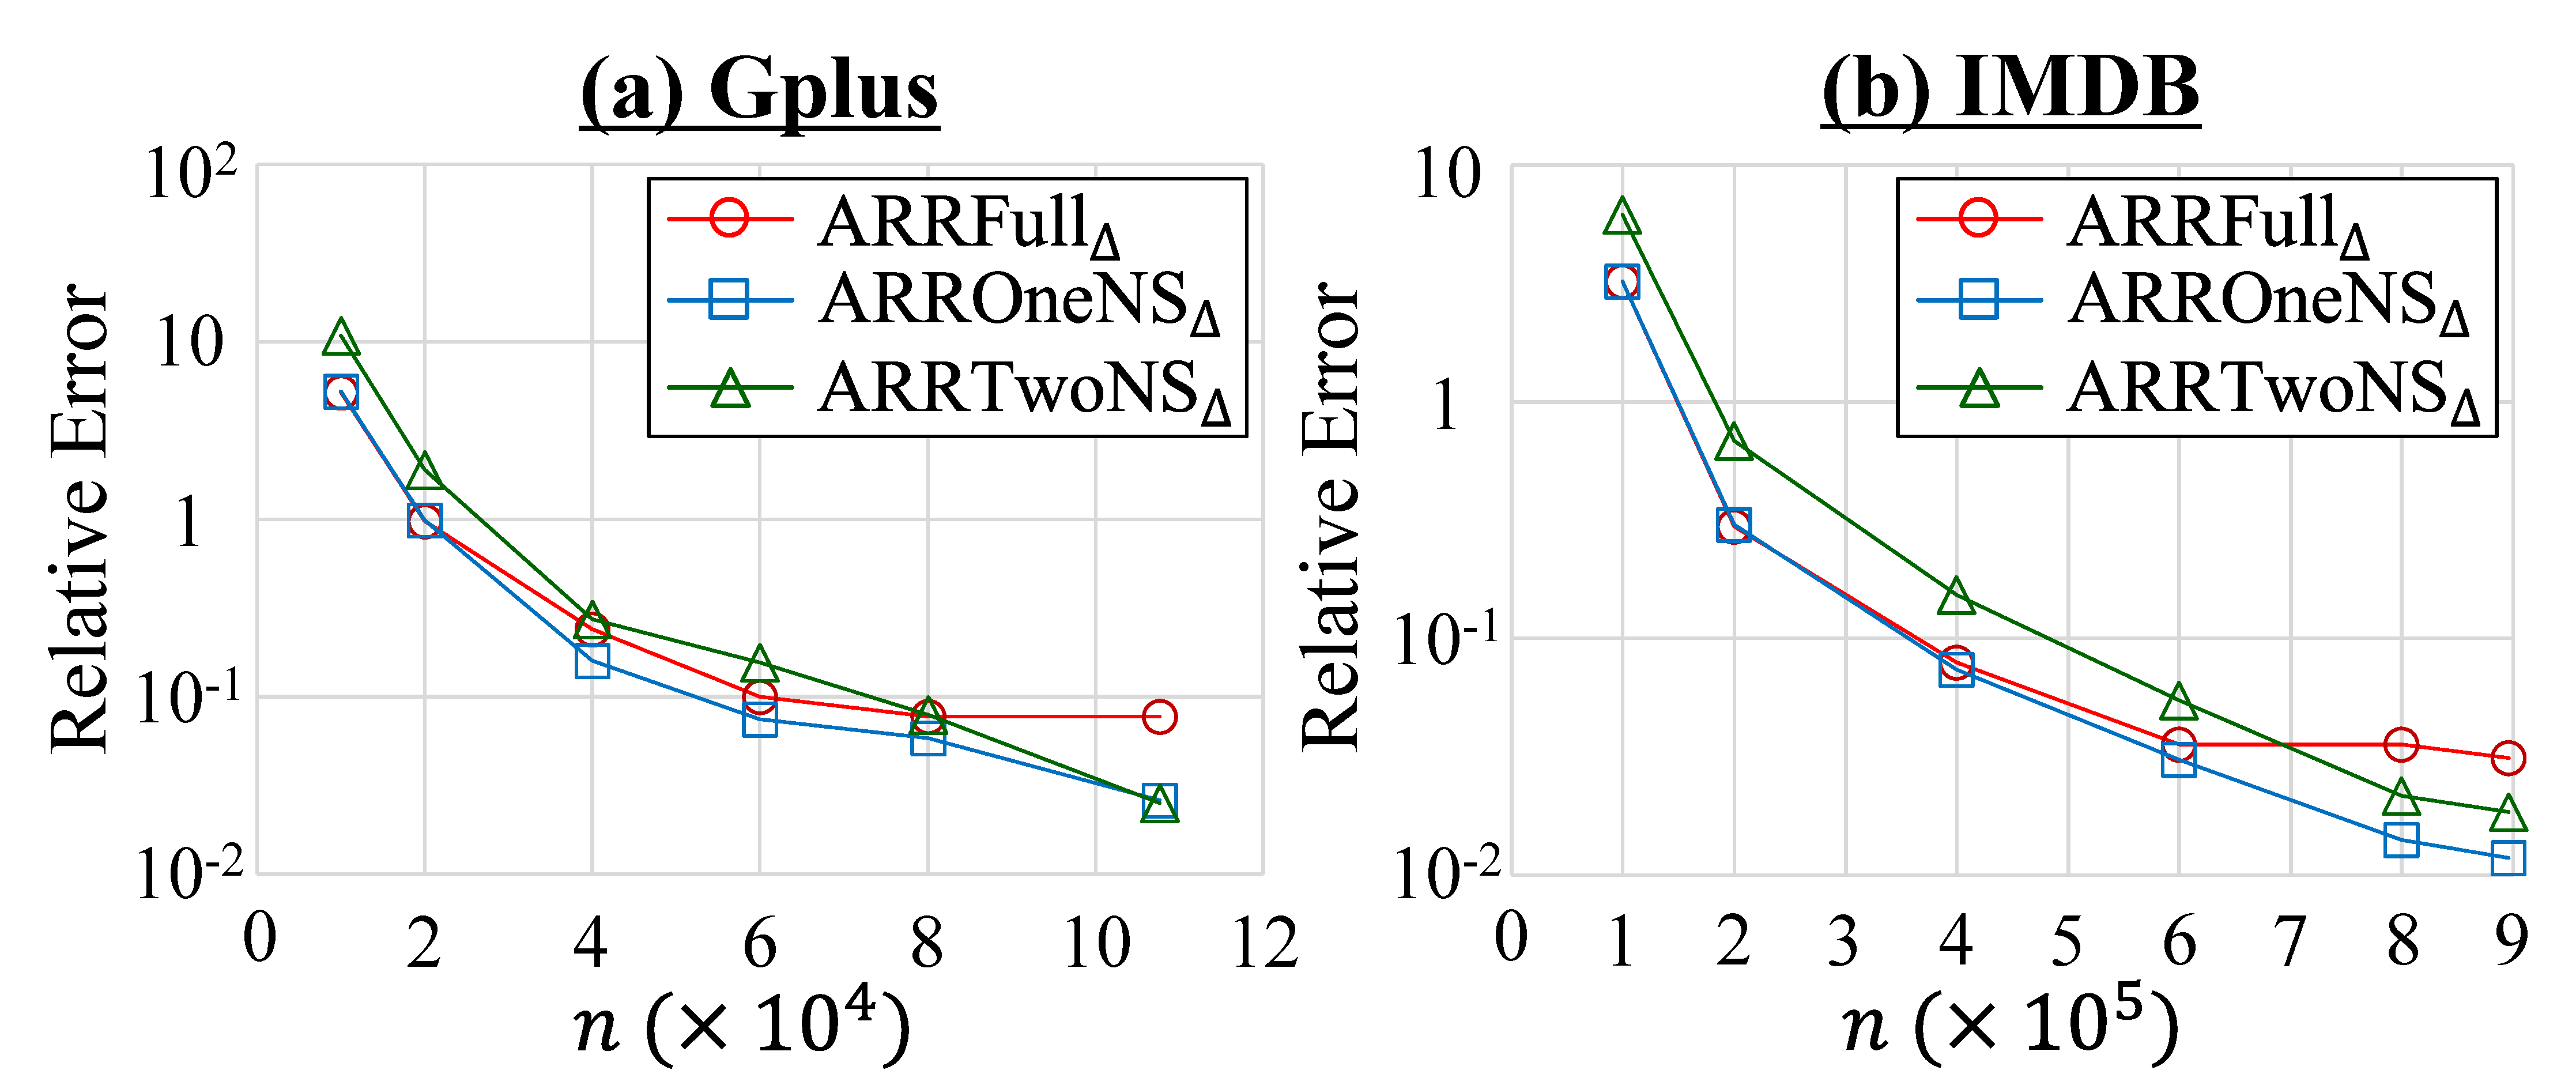
\includegraphics[width=0.99\linewidth]{fig/res3_n.pdf}
  \vspace{-4mm}
  \caption{Relative error of our three algorithms with double clipping for various values of $n$ 
  ($\epsilon=1$, $\mu^*=10^{-3}$).} 
  \label{chap2-fig:res3_n}
\end{figure}

Figure~\ref{chap2-fig:res3_n} shows the results, where $\epsilon=1$ ($\epsilon_0=0.1$, $\epsilon_1 = \epsilon_2 = 0.45$) and $\mu^* = 10^{-3}$. 
In all 
% the 
three algorithms, the relative error decreases with increase in $n$.
This is because the expected $l_2$ loss can be expressed as 
% $O(n)$ (when we regard $\epsilon$ and $\mu_F$ as constants and ignore $d_{max}$) 
$O(n d_{max}^3)$ or $O(n d_{max}^2)$ 
% (when we regard $\epsilon$ as constants) 
in these algorithms as shown in Section~\ref{chap2-sub:clip_theoretical_analysis} and the square of the true triangle count can be expressed as $\Omega(n^2)$.
In other words, when $d_{max} \ll n$, the relative error becomes smaller for larger $n$. 
% In other words, this is consistent with our theoretical results. 
Figure~\ref{chap2-fig:res3_n} also shows that for small $n$, \AlgThree{} provides the worst performance and 
\AlgTwo{} performs almost the same as \AlgOne{}. 
% the difference between \AlgTwo{} and \AlgOne{} is very small. 
For large $n$, 
% \AlgThree{} outperforms \AlgOne{} and 
\AlgOne{} performs the worst and 
\AlgTwo{} performs the best. 


To investigate the reason for this, we decomposed the estimation error into two components -- 
the first error caused by empirical estimation and the second error caused by the Laplacian noise. 
Specifically, for each algorithm, 
we evaluated the first error by calculating the relative error when we did not add the Laplacian noise ($\epsilon_1 = 0.45$). 
Then we evaluated the second error by subtracting the first error from the relative error when we used double clipping ($\epsilon_0=0.1$, $\epsilon_1 = \epsilon_2 = 0.45$). 

Figure~\ref{chap2-fig:res3_emp_Lap} shows the results for some values of $n$, where ``emp'' represents the first error by empirical estimation and ``Lap'' represents the second error by the Laplacian noise. 
We observe that the second error 
rapidly decreases with increase in $n$. 
% The difference between \AlgOne{} and \AlgTwo{} 
% This is because the expected $l_2$ loss of the Laplacian noise is $O(\sum_{i=1}^n \kappa_i^2)$, 
% which is much smaller than $O(n d_{max}^2)$, 
% as shown in Section~\ref{chap2-sub:clip_theoretical_analysis}. 
In addition, 
% Figure~\ref{chap2-fig:res3_emp_Lap} also shows that 
the first error of \AlgOne{} is much larger than those of \AlgTwo{} and \AlgThree{} when $n$ is large. 

We also examined 
% the maximum degree $d_{max}$ and 
the number $C_4$ of $4$-cycles as a function of $n$. Figure~\ref{chap2-fig:res4_4cycles} shows the results. 
We observe that $C_4$ (which is $O(n d_{max}^3)$) is quartic in $n$; e.g., $C_4$ is increased by $2^4 \approx 10$ and $6^4 \approx 10^3$ when $n$ is multiplied by $2$ and $6$, respectively. 
This is because we randomly selected $n$ users from all users and $d_{max}$ is almost proportional to $n$ (though $d_{max} \ll n$). 
% We observe that $d_{max}$ is proportional to $n$ (though $d_{max} \ll n$). 
% This is because we randomly selected $n$ users from all users. 
% Consequently, $C_4$ which can be expressed as $O(n d_{max}^3)$ is quartic in $n$; e.g., $C_4$ is increased by $2^4 \approx 10$ and $6^4 \approx 10^3$ when $n$ is multiplied by $2$ and $6$, respectively. 

\begin{figure}[t]
  \centering
  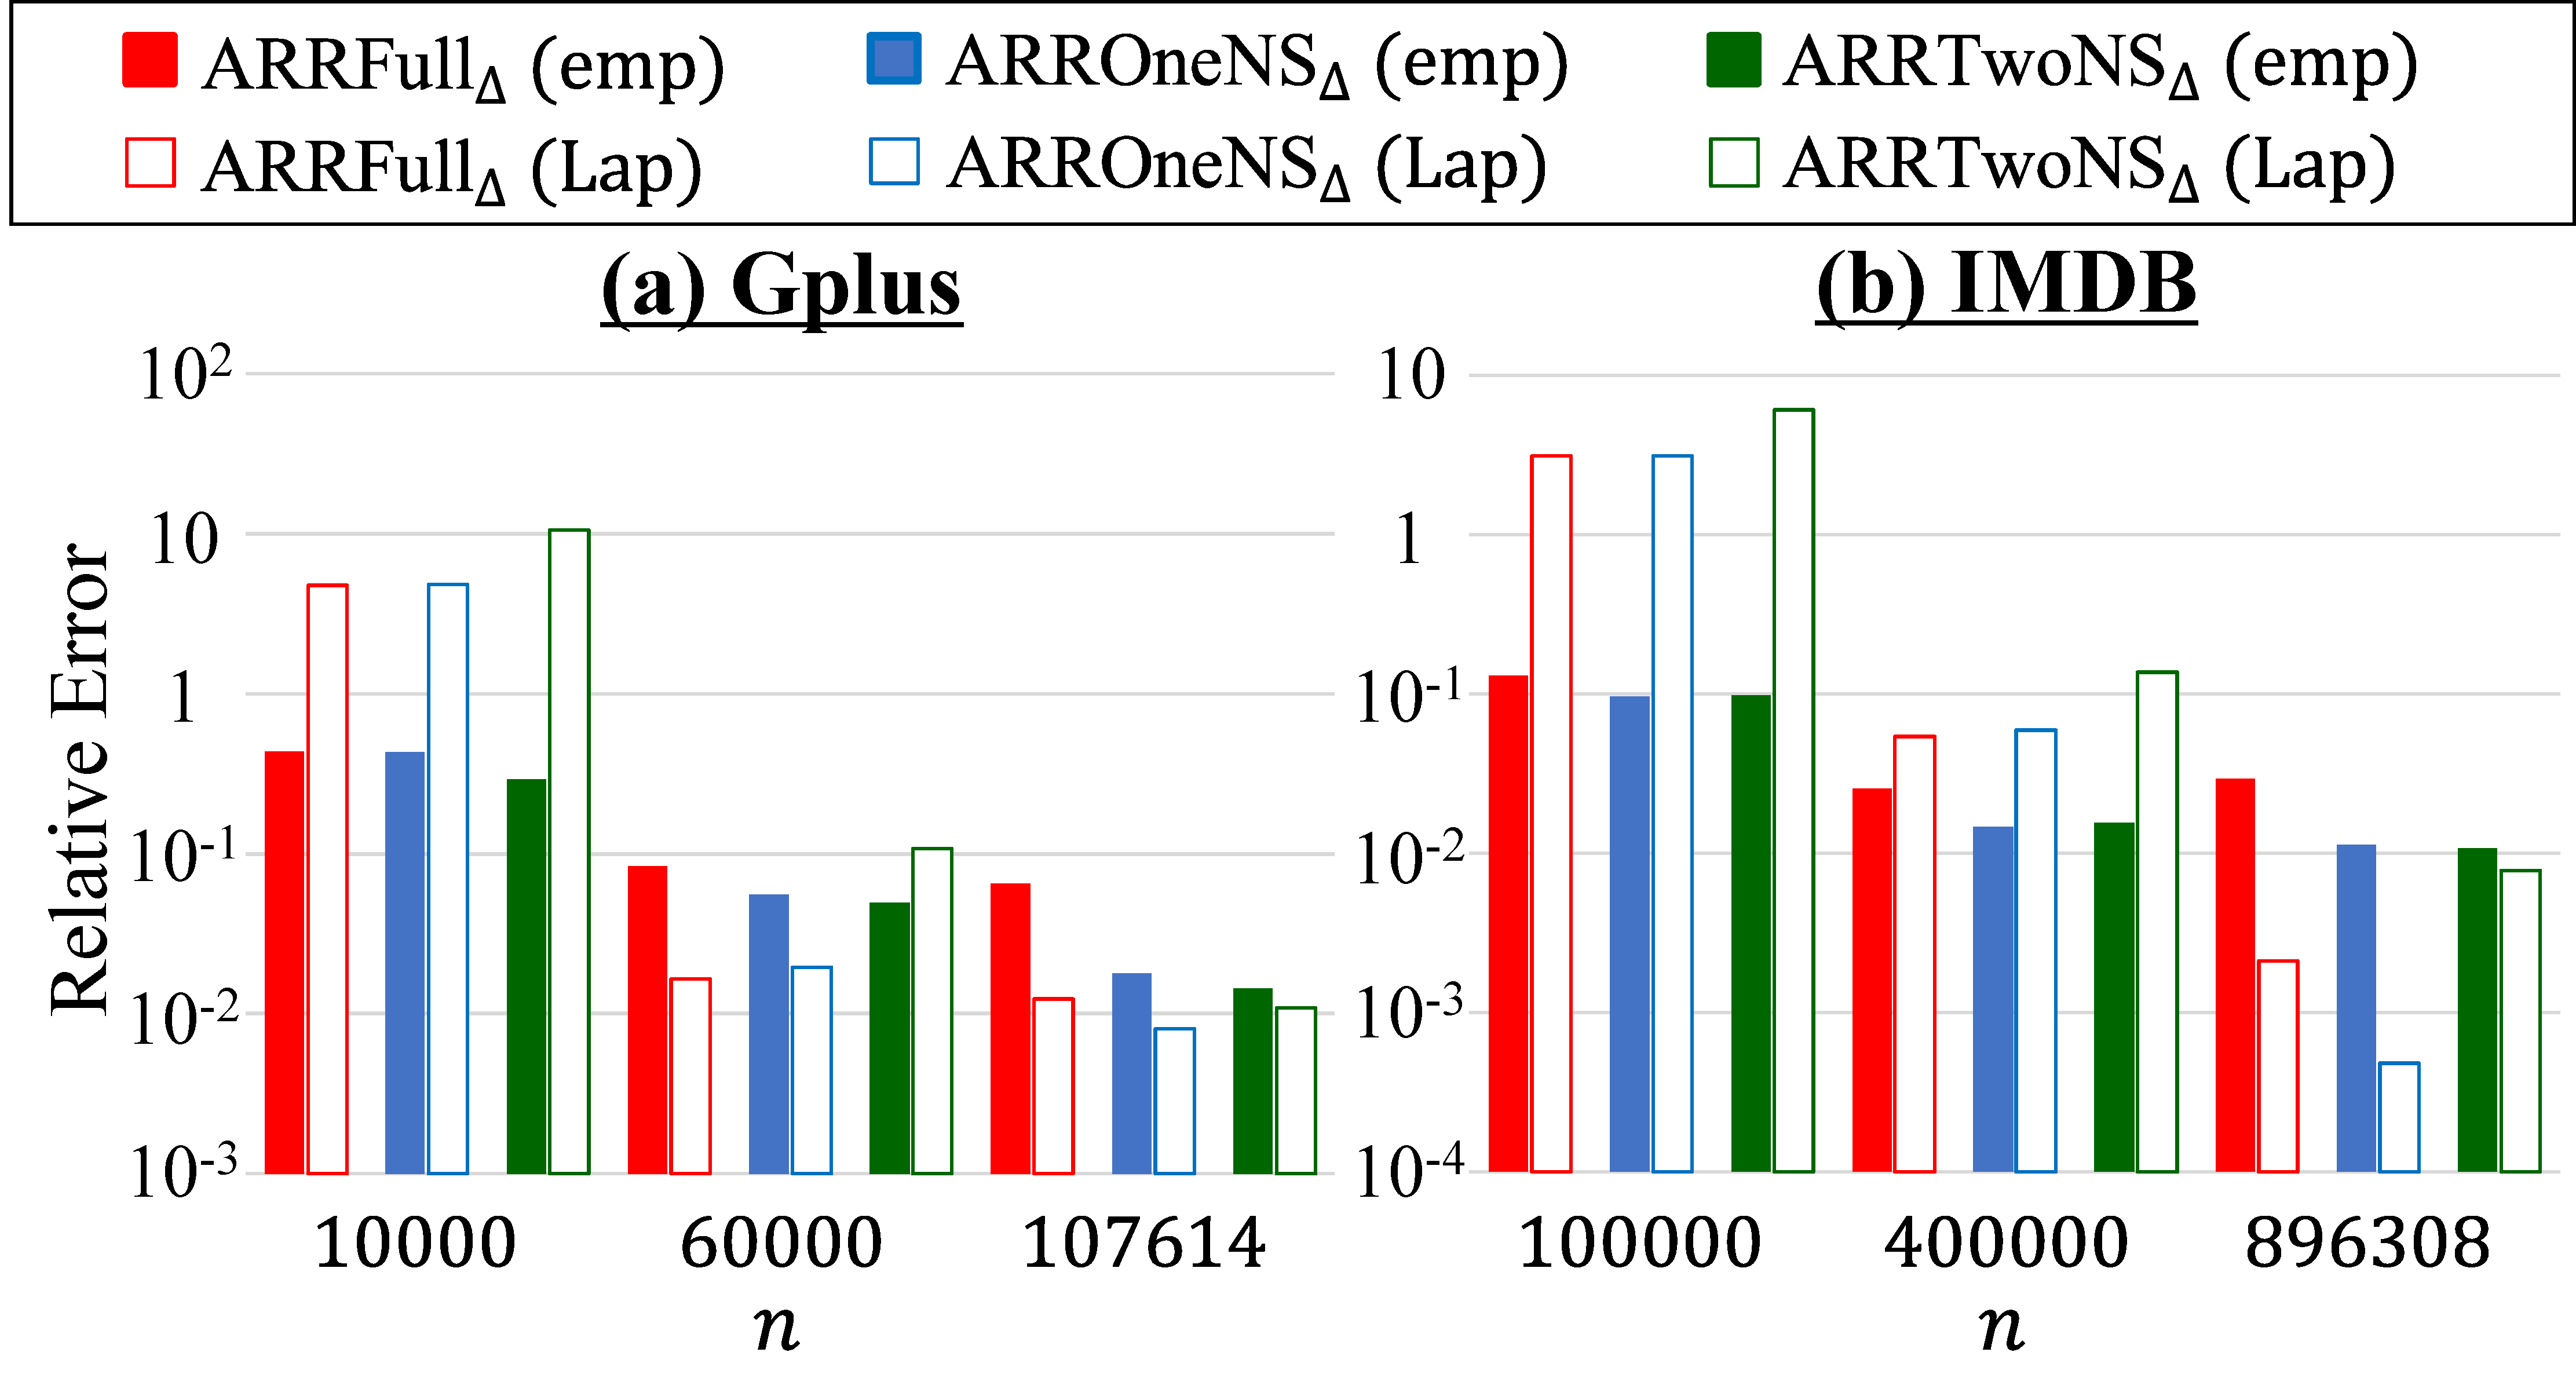
\includegraphics[width=0.99\linewidth]{fig/res3_emp_Lap.pdf}
  \vspace{-5mm}
  \caption{Relative error of empirical estimation and the Laplacian noise in our three algorithms with double clipping ($\epsilon=1$, $\mu^*=10^{-3}$).} 
  \label{chap2-fig:res3_emp_Lap}
% \end{figure}
 \vspace{1mm}
% \begin{figure}[t]
  \centering
  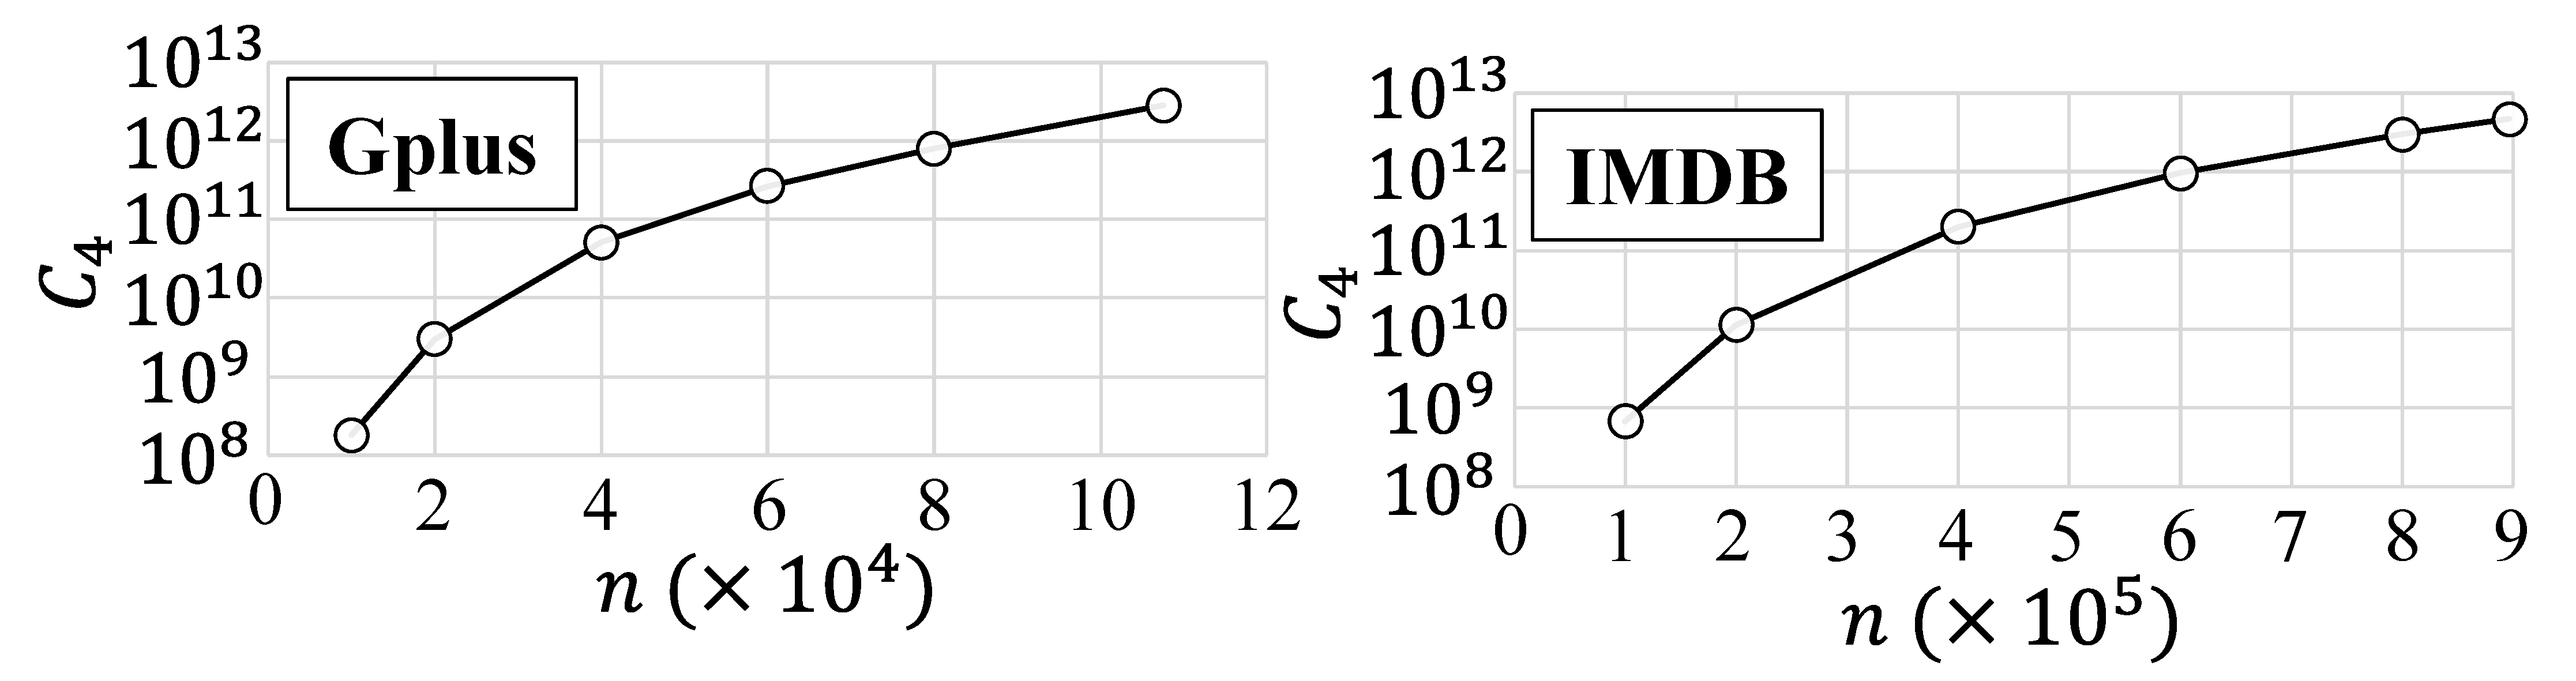
\includegraphics[width=0.99\linewidth]{fig/res4_4cycles.pdf}
  \vspace{-5mm}
%   \caption{Maximum degree $d_{max}$ and \#$4$-cycles $C_4$.} 
  \caption{\#$4$-cycles $C_4$.} 
  \label{chap2-fig:res4_4cycles}
\end{figure}

Based on Figures~\ref{chap2-fig:res3_emp_Lap} and \ref{chap2-fig:res4_4cycles}, we can explain 
% the results in 
Figure~\ref{chap2-fig:res3_n} as follows. 
As shown in Section~\ref{chap2-sub:clip_theoretical_analysis}, the $l_2$ loss of empirical estimation can be expressed as 
% $O(\frac{n d_{max}^3}{\mu_F})$, $O(\frac{n d_{max}^2}{\mu_O^2})$, and $O(\frac{n d_{max}^2}{\mu_T^3})$ 
$O(n d_{max}^3)$, $O(n d_{max}^2)$, and $O(n d_{max}^2)$ 
in \AlgOne{}, \AlgTwo{}, and \AlgThree{}, respectively. 
% when 
% we regard $\epsilon$ as a constant.
% $\mu_F$ ($= \mu_O^2 = \mu_T^3$) 
% $\mu^*$ is small.  
The large $l_2$ loss of \AlgOne{} is caused by a large value of $C_4$. 
% as shown in Figure~\ref{chap2-fig:res4_4cycles}. 
% the $4$-cycle issue. 
% When 
% $\mu_F$ is small, 
% $n$ is small, 
% the Laplacian noise has a non-negligible impact on the estimation error. 
% as explained in Section~\ref{chap2-sub:clip_theoretical_analysis}. 
% However, 
The expected $l_2$ loss of the Laplacian noise is 
$O(\sum_{i=1}^n \kappa_i^2)$, 
% $O(\sum_{i=1}^n \lambda_i^2 \td_i^2)$, 
which is much smaller than $O(n d_{max}^2)$. 
Thus, 
% when $n$ is large, 
as $n$ increases, 
% when $d_{max}$ is proportional to $n$, 
% as in Figure~\ref{chap2-fig:res4_4cycles}, 
the Laplacian noise becomes relatively very small, 
% rapidly decreases with increase in $n$ 
as shown in Figure~\ref{chap2-fig:res3_emp_Lap}. 
Consequently, \AlgTwo{} provides the best performance for large $n$ because it addresses the $4$-cycle issue 
and effectively reduces the global sensitivity. 
This explains the results in Figure~\ref{chap2-fig:res3_n}. 
It is also interesting that when $n \approx 10^5$, \AlgOne{} performs the worst in \GPlus{} and almost the same as \AlgTwo{} in \IMDB{} (see Figure~\ref{chap2-fig:res3_n}). 
This is because \GPlus{} is more dense than \IMDB{} 
% (as described in Section~\ref{chap2-sub:setup}) 
and $C_4$ is much larger in \GPlus{} when $n \approx 10^5$, as in Figure~\ref{chap2-fig:res4_4cycles}.

In other words, Figures~\ref{chap2-fig:res3_n}, \ref{chap2-fig:res3_emp_Lap}, and \ref{chap2-fig:res4_4cycles} are consistent with our theoretical results in Section~\ref{chap2-sub:clip_theoretical_analysis}. 
From these results, we conclude that \AlgTwo{} is effective especially for 
a large graph (e.g., $n \approx 10^6$) or dense graph (e.g., \GPlus{}) where the number $C_4$ of $4$-cycles is large. 
% a graph that has a large number of $4$-cycles. 
% In Appendix~\ref{chap2-sec:BAmodel}, we also show similar results using the Barab\'{a}si-Albert graph model.



% \smallskip
% \noindent{\textbf{Communication Cost.}}~~TBD.

\smallskip
\noindent{\textbf{Summary.}}~~In summary, our answers to our three research questions RQ1-3 
% at the beginning of Section~\ref{chap2-sec:experiments} 
are as follows. 
% \begin{itemize}
%     \item Our 
% \end{itemize}
% First, 
[RQ1]: Our \AlgTwo{} achieves almost the smallest estimation error in all cases and outperforms the other two, especially for a large graph or dense graph where $C_4$ is large. 
[RQ2]: Our double clipping reduces the estimation error by two or three orders of magnitude. 
[RQ3]: Our entire algorithm (\AlgTwo{} with double clipping) dramatically reduces the communication cost, 
e.g., 
% from $400$ Gbits to $160$ Mbits or less (relative error $=0.21$) in \IMDB{}.
% When the DL speed is $20$ Mbps \cite{YouTube_speed}, the DL time is reduced from $6$ hours to $5$ seconds. 
from $6$ hours to $8$ seconds or less (relative error $=0.21$) in \IMDB{} at a $20$ Mbps download rate \cite{YouTube_speed}. 

Thus, triangle counting under edge LDP is now 
much more 
practical. 
In Appendix~\ref{chap2-sec:cluster}, we show that the clustering coefficient can also be accurately estimated using our algorithms.


\section{Conclusions}
\label{chap2-sec:conclusions}
% In this paper, we proposed
% locally private
We proposed
triangle counting algorithms under edge LDP with a small estimation error and small communication cost.
We showed that
% the estimation error can be significantly reduced by our 4-cycle trick and double clipping, and that
our entire algorithms with the 4-cycle trick and double clipping
% can 
dramatically reduce the download cost
% when compared with
of
\cite{Imola_USENIX21},
% (e.g., from $400$ Gbits to $100$ Mbits).
e.g., from 6 hours to 8 seconds or less. 
% when $20$ Mbps).
% In \cite{Imola_USENIX21},

% In this paper,
We assumed that each user $v_i$ honestly inputs her neighbor list $\bma_i$, as in most previous work on LDP.
However, recent studies \cite{Cao_USENIX21,Cheu21} show that the estimate in LDP can be skewed by data poisoning attacks.
% with a number of malicious accounts.
As future work, we would like to analyze the impact of data poisoning on our algorithms and develop defenses (e.g., detection) against it.


% %-------------------------------------------------------------------------------
\section*{Acknowledgments}
Kamalika Chaudhuri and Jacob Imola would like to thank ONR under N00014-20-1-2334 and UC Lab Fees under LFR 18-548554  for research support.
Takao Murakami was supported in part by JSPS KAKENHI JP19H04113.


